% !TEX root = ../thesis.tex

\section{Systematic Uncertainties}
\label{sec:uncert}

% Uncertainties overview
To implement systematic uncertainties in the analysis, we introduce nuisance parameters into the 2D fit that allow for changes to the shapes and normalizations for the signal and background models.
In this section, we discuss the nuisance parameters that are applied to the signal and background processes, and how they are correlated between different categories.

\subsection{Signal Normalization}

% Signal normalization
The signal normalization uncertainties are 100\% correlated between search categories unless otherwise stated.
\begin{itemize}
  \item {\bfseries Luminosity:} Normalization uncertainty of 1.8\% as recommended by the Luminosity POG~\cite{LumiPOG}.
  \item {\bfseries PDF:} Normalization uncertainty of 1\%.
  The scale uncertainties were evaluated as prescribed by references~\cite{Cacciari_2004,Catani_2003}.
  For the PDF uncertainties, we follow the recommendations from the NNPDF 3.0 PDF set~\cite{Ball2011296}.
  The uncertainties obtained in acceptance were found to be less than 0.1\% for the scale variation, and 0.1-0.9\% for the PDF evaluation.
  \item {\bfseries Pileup reweighting:} Normalization uncertainty of 1.5\%, estimated by shifting the minimum bias cross section by 4.6\% and deriving alternative pileup weights.
  \item {\bfseries Lepton ID and trigger efficiency:} Normalization uncertainty of 5\% for the electron and muon channels separately.
  This is 100\% correlated to a parameter for the resonant background, but uncorrelated with a similar parameter for the non-resonant background.
  \item {\bfseries $b$-tag fake rate:} Normalization uncertainty of 2\% accounting for modeling the no-$b$ tag requirement.
  \item {\bfseries $V$-tagging efficiency:} Normalization uncertainty for the scale factors $SF^{\mathrm{HP}/\mathrm{LP}}$ for the efficiency of the \nsubjDDT selection, with $\pm4\%$ in HP and $\mp4\%$ in LP\footnote{The HP and LP uncertainties have opposite signs due to the fact that they are anti-correlated}.
  \item {\bfseries Momentum dependence of the $V$-tagging efficiency:} Normalization uncertainty arising from the extrapolation of the $V$-tagging efficiency scale factors.
  We fit the \MX dependence of the $V$-tagging efficiency as seen in figure~\ref{fig:VTag_massdep_summary} (right) and subtract the efficiency at $650\unit{GeV}$ to obtain an \MX-dependent uncertainty for the HP and LP categories given by:
  \begin{itemize}
    \item $\pm(4.95\times10^{-3})[(\MX-650\unit{GeV})/(1\unit{GeV})]$ in the HP category.
    \item $\mp(3.54\times10^{-3})[(\MX-650\unit{GeV})/(1\unit{GeV})]$ in the LP category.
  \end{itemize}
  \item {\bfseries \bbbar-tagging efficiency:} Normalization uncertainty on the scale factors for the efficiency on the cut of the \bbbar-tagger obtained by shifting the scale factors up and down and propagating the results to the expected signal yields.
  This results in the following uncertainties:
  \begin{itemize}
    \item $\pm9\%$ (bb) / $\mp0.4\%$ (nobb) for the \WW signals.
    \item $\pm9\%$ (bb) / $\mp1.5\%$ (nobb) for the \WZ signals.
    \item $\pm6\%$ (bb) / $\mp2.5\%$ (nobb) for the \WH signal.
  \end{itemize}
  \item {\bfseries \Dy cut efficiency:} Normalization uncertainty for the efficiency of the cut at $\Dy=1.0$ separating the LDy and HDy categories.
  This is estimated by fitting a linear function to the data/MC ratio for the distribution of \Dy in the top-enriched control region, then linearly reweighing the signal distribution of \Dy for each signal model, using the slope obtained from the data/MC fit and using a $y$-intercept that keeps the total integral of the signal distribution constant.
  Taking the signal efficiency in LDy and HDy as the 1-$\sigma$ up uncertainty, we obtain the following:
  \begin{itemize}
    \item $+4\%$ (HDy) / $-1.5\%$ (LDy) for \ggF\GBulktoWW.
    \item $+4\%$ (HDy) / $-3.5\%$ (LDy) for \ggF and \VBF\RadtoWW, and \DY\ZprtoWW.
    \item $+4\%$ (HDY) / $-2\%$ (LDy) for \DY\WprtoWZ and \WprtoWH.
    \item $+6\%$ (HDy) / $-5\%$ (LDy) for \VBF\GBulktoWW.
    \item $+2\%$ (HDy) / $-5.5\%$ (LDy) for \VBF\ZprtoWW and \WprtoWZ.
  \end{itemize}
\end{itemize}

\subsection{Signal Shape}

% MVV signal shape
For the signal shapes, we implement nuisance parameters to the $\MVV$ shape as relative scale factors on the mean $\mu$ and standard deviation $\sigma$ of the DCB function.
Each of the following $\MVV$ shape parameters are 100\% correlated across the categories in which they apply:
\begin{itemize}
  \item {\bfseries Jet energy scale and resolution:} 2\% for the scale and 5\% for the resolution.
  \item {\bfseries Missing transverse energy scale and resolution:} 2\% for the scale and 1\% for the resolution.
  \item {\bfseries Electron and muon energy scale:} 0.5\% for the electron channel and 0.3\% for the muon channel.
\end{itemize}

% MJ signal shape
The \MJ signal shape is affected by the uncertainty on the scale and resolution for the soft drop mass.
To obtain these uncertainties, we correct the central values of the \MJ scale and resolution parameters with the factors of 0.989 and 1.08 obtained for Run 2 in table~\ref{tab:VScaleRes}.
The soft drop mass scale and resolution uncertainties obtained are the following:
\begin{itemize}
  \item {\bfseries Soft drop mass scale and resolution:} 1\% for the scale and 8\% for the resolution.
\end{itemize}
The resulting uncertainties are 100\% correlated between the electron and muon channels, between the bb, nobb, and vbf categories, and between the LDy and HDy categories, but not the HP and LP categories.

\subsection{Background Normalization}

% Background normalization
We use two sets of nuisance parameters for the background normalization:
\begin{itemize}
  \item A 5\% normalization uncertainty uncorrelated between the electron and muon channels, but 100\% correlated between the resonant and non-resonant background, between the HP and LP categories, between the bb, nobb, and vbf categories, and between the LDy and HDy categories.
  \item A 25\% normalization uncertainty uncorrelated between the resonant and non-resonant background, between the HP and LP categories, between the bb, nobb, and vbf categories, and between the LDy and HDy categories, but 100\% correlated between the muon and electron channels.
\end{itemize}

\subsection{Non-resonant Background Shape}

% Non-resonant conditional shape variation
We define two shape variations for the conditional part of the likelihood for the 2D fitting process to account for the differences between data and simulation:
\begin{itemize}
  \item {\bfseries Jet \pt spectrum:} Derived by reweighting the jet \pt spectrum to be harder or softer.
  It affects only the \MVV dimension and is motivated by higher order corrections in the \Wjets production not modeled by the simulation.
  \item {\bfseries Diagonal:} Modifies the correlation between the jet mass and the jet \pt.
  The variation changes the slope of the linear part of figure~\ref{fig:nonRes2DCorr}.
\end{itemize}
Both of these shape variations are left uncorrelated across categories due to the fact that they are sensitive to different regions of the PDFs.
The projections of the nominal and $\pm3\sigma$ alternative 2D shapes onto the \MVV dimension for the jet \pt spectrum and diagonal uncertainties are shown in figures~\ref{fig:systNonResMVV_MVVScale} and \ref{fig:systNonResMVV_Diag}.

\begin{figure}[htbp]
  \centering
  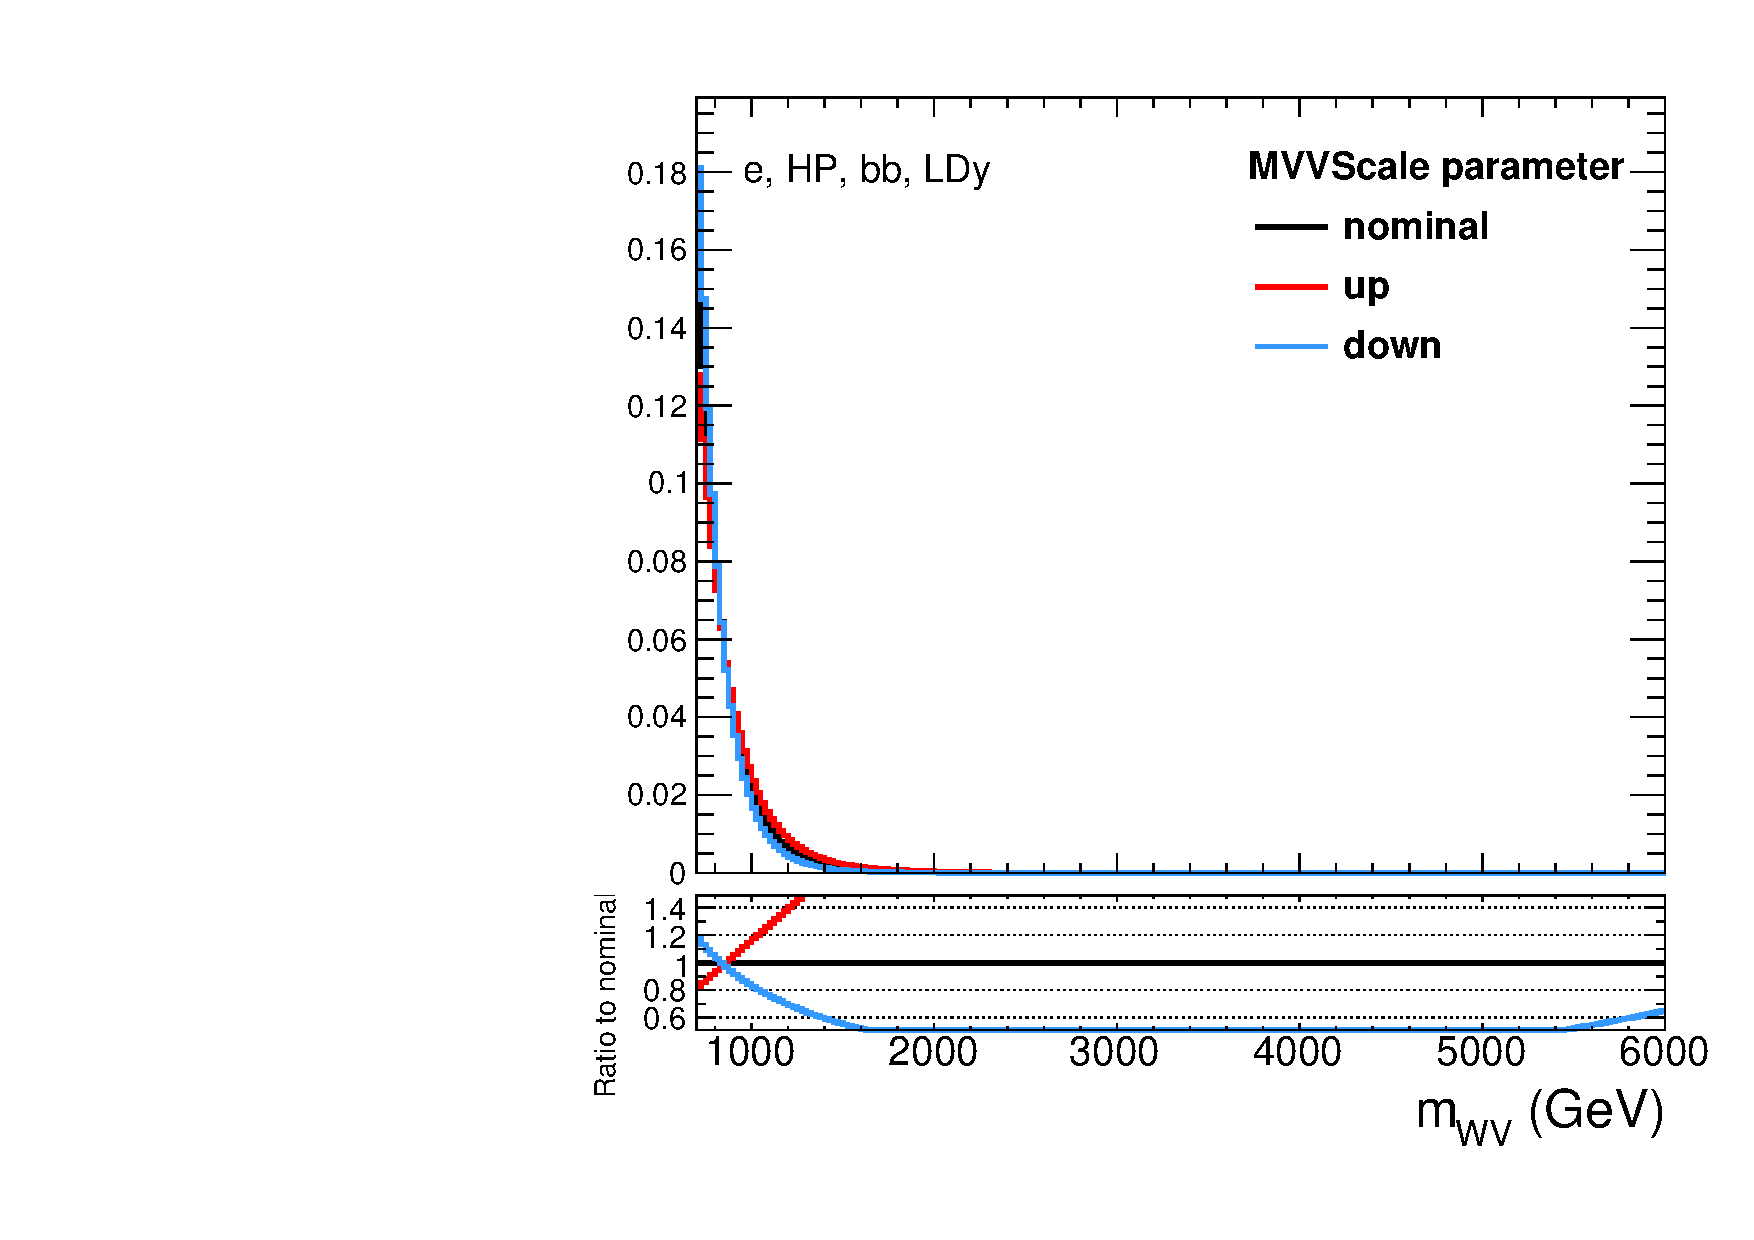
\includegraphics[width=0.21\textwidth]{fig/uncertainties/systs_nonRes_e_HP_bb_LDy_MVVScale_ProjX.pdf}
  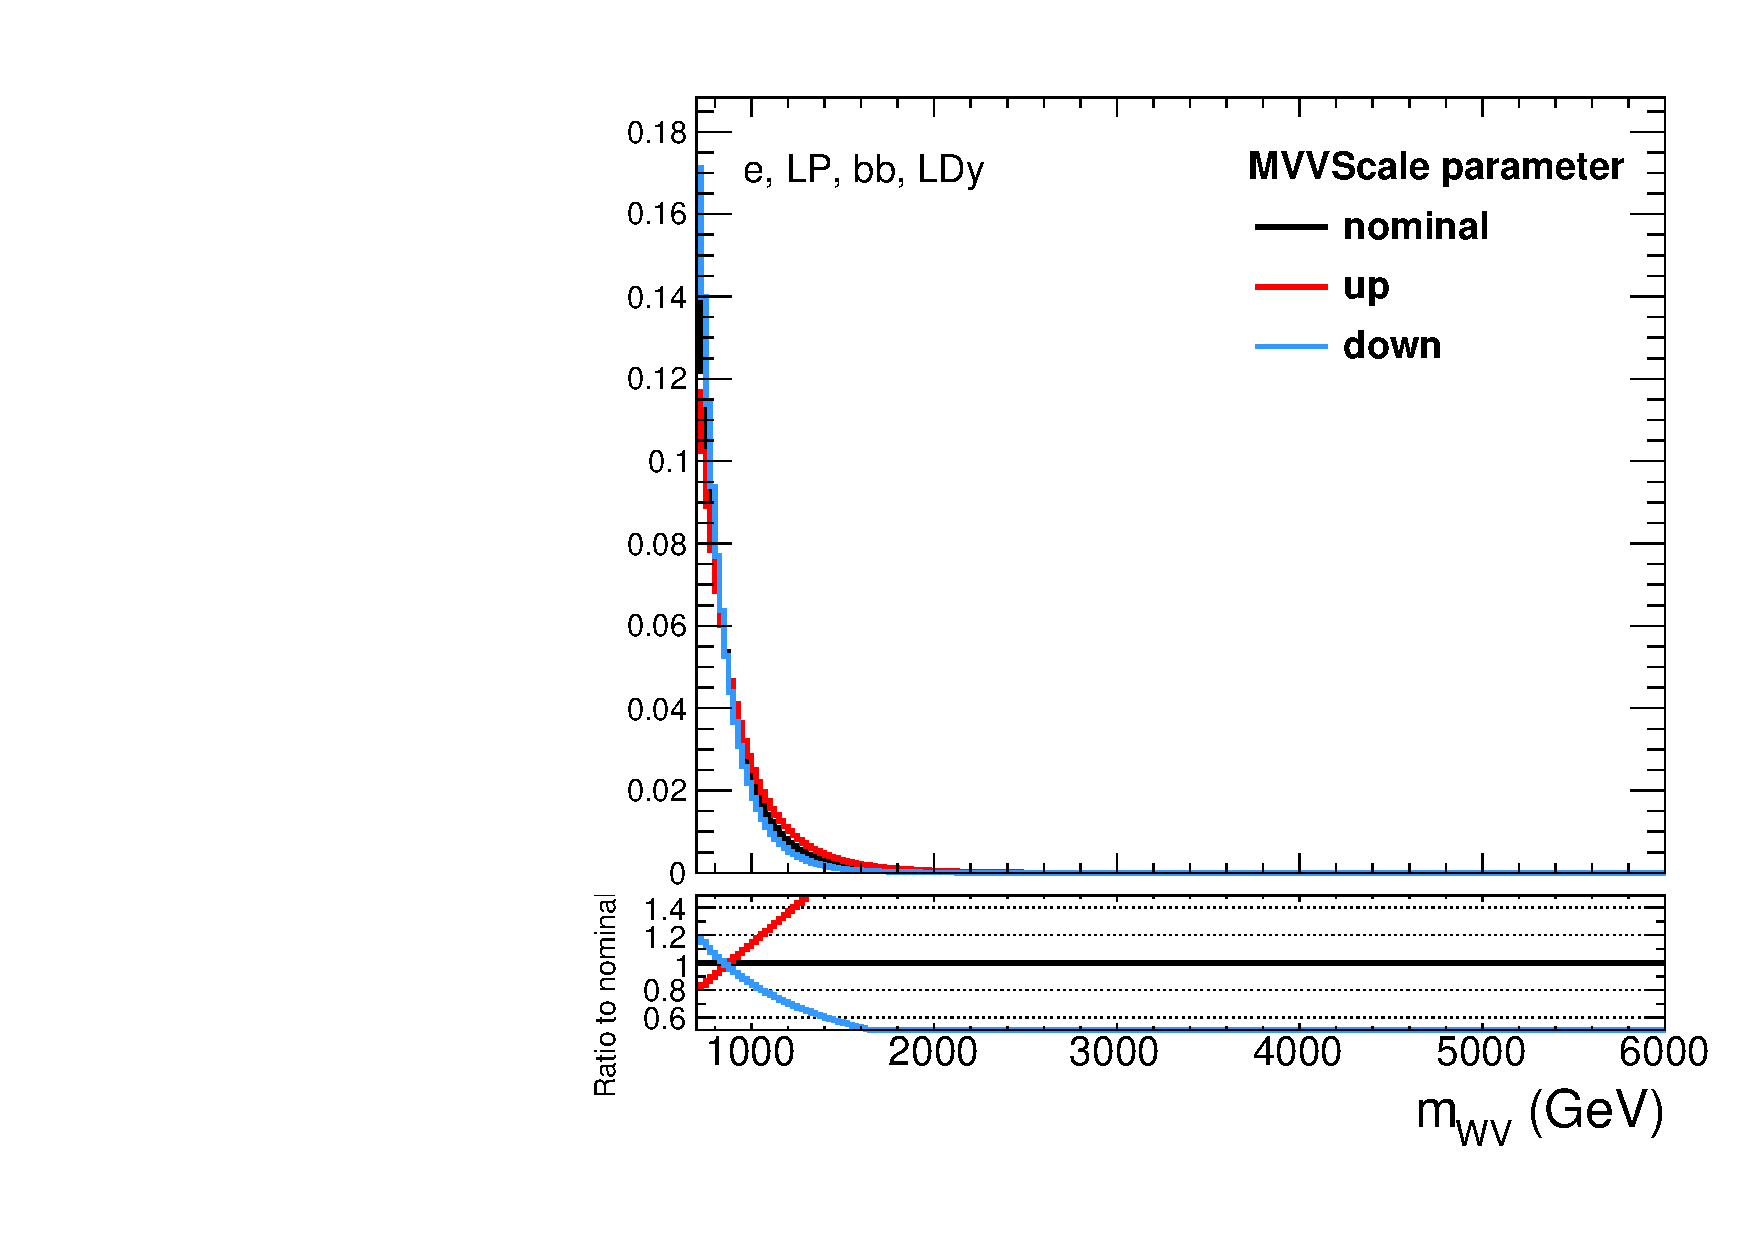
\includegraphics[width=0.21\textwidth]{fig/uncertainties/systs_nonRes_e_LP_bb_LDy_MVVScale_ProjX.pdf}
  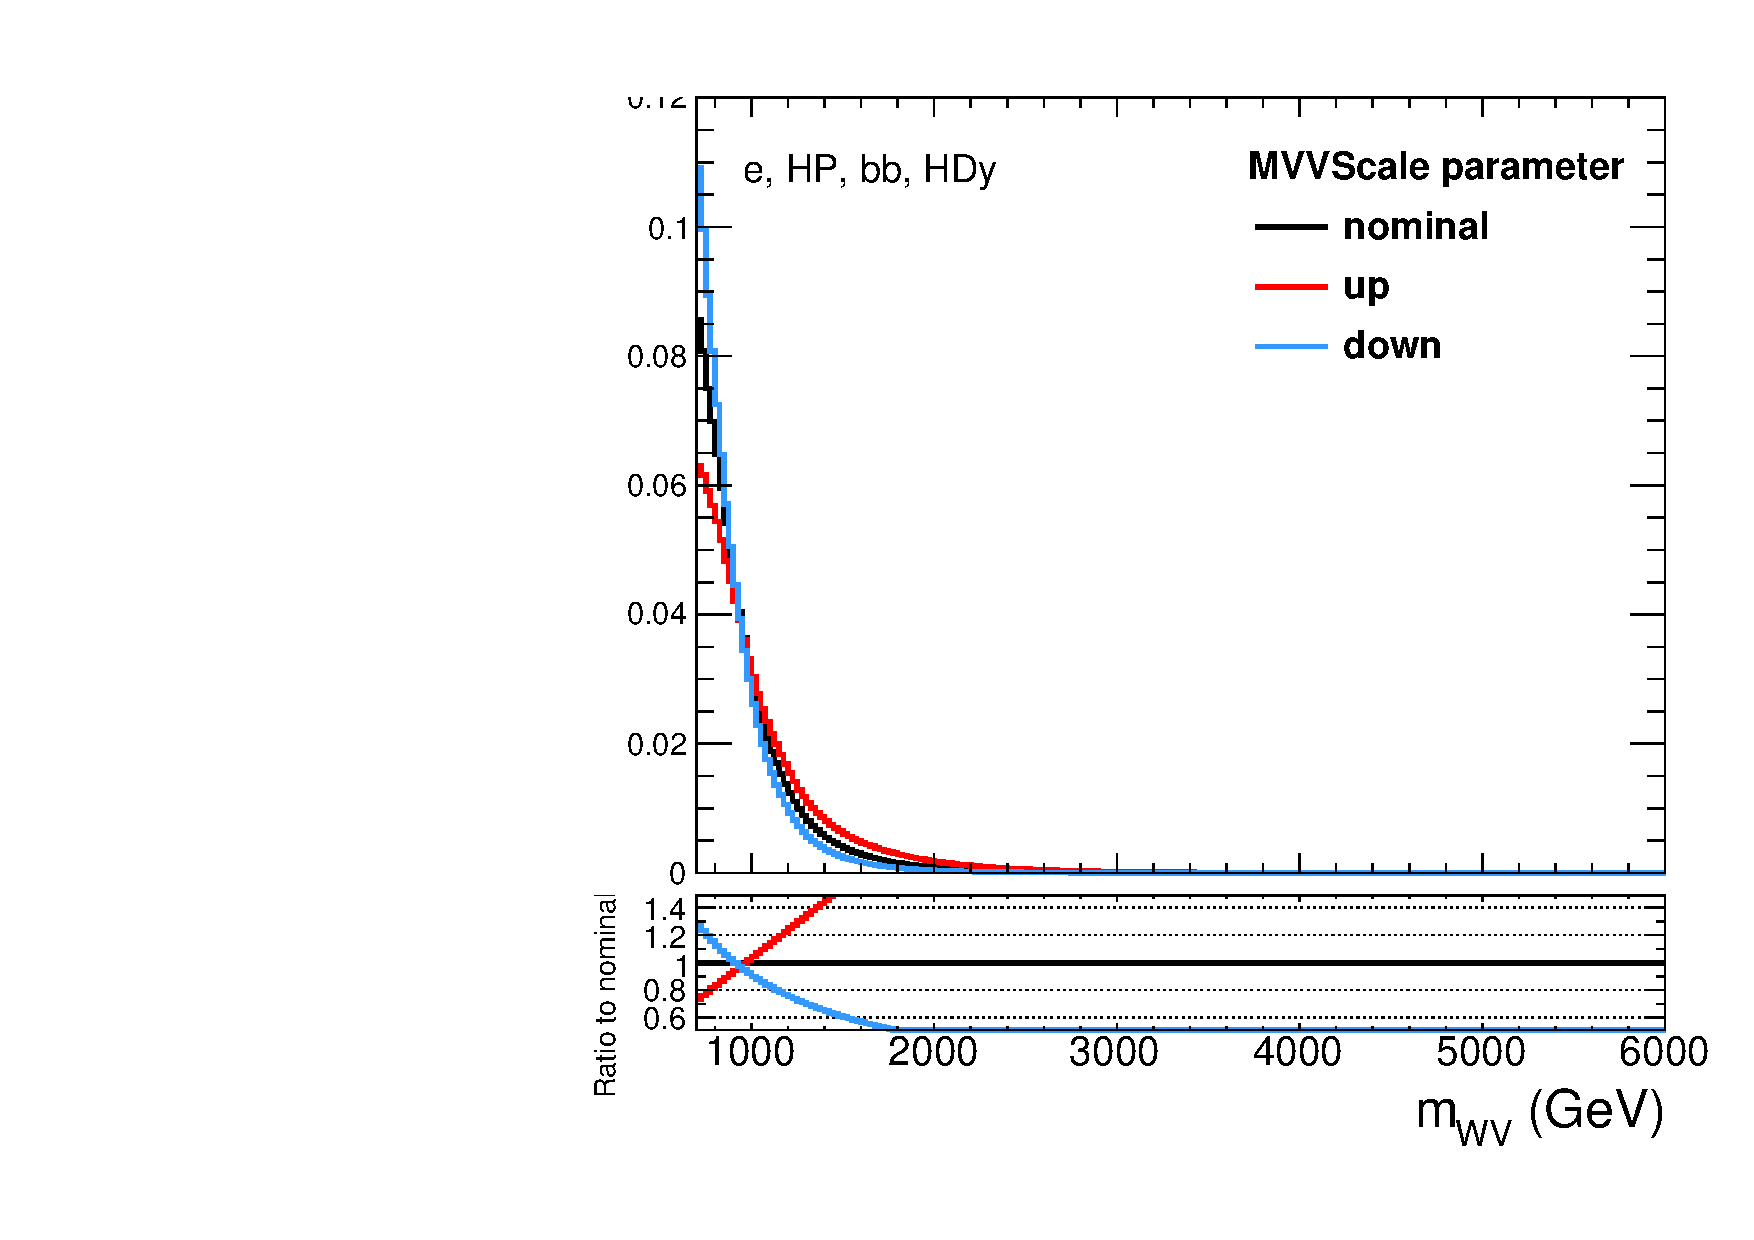
\includegraphics[width=0.21\textwidth]{fig/uncertainties/systs_nonRes_e_HP_bb_HDy_MVVScale_ProjX.pdf}
  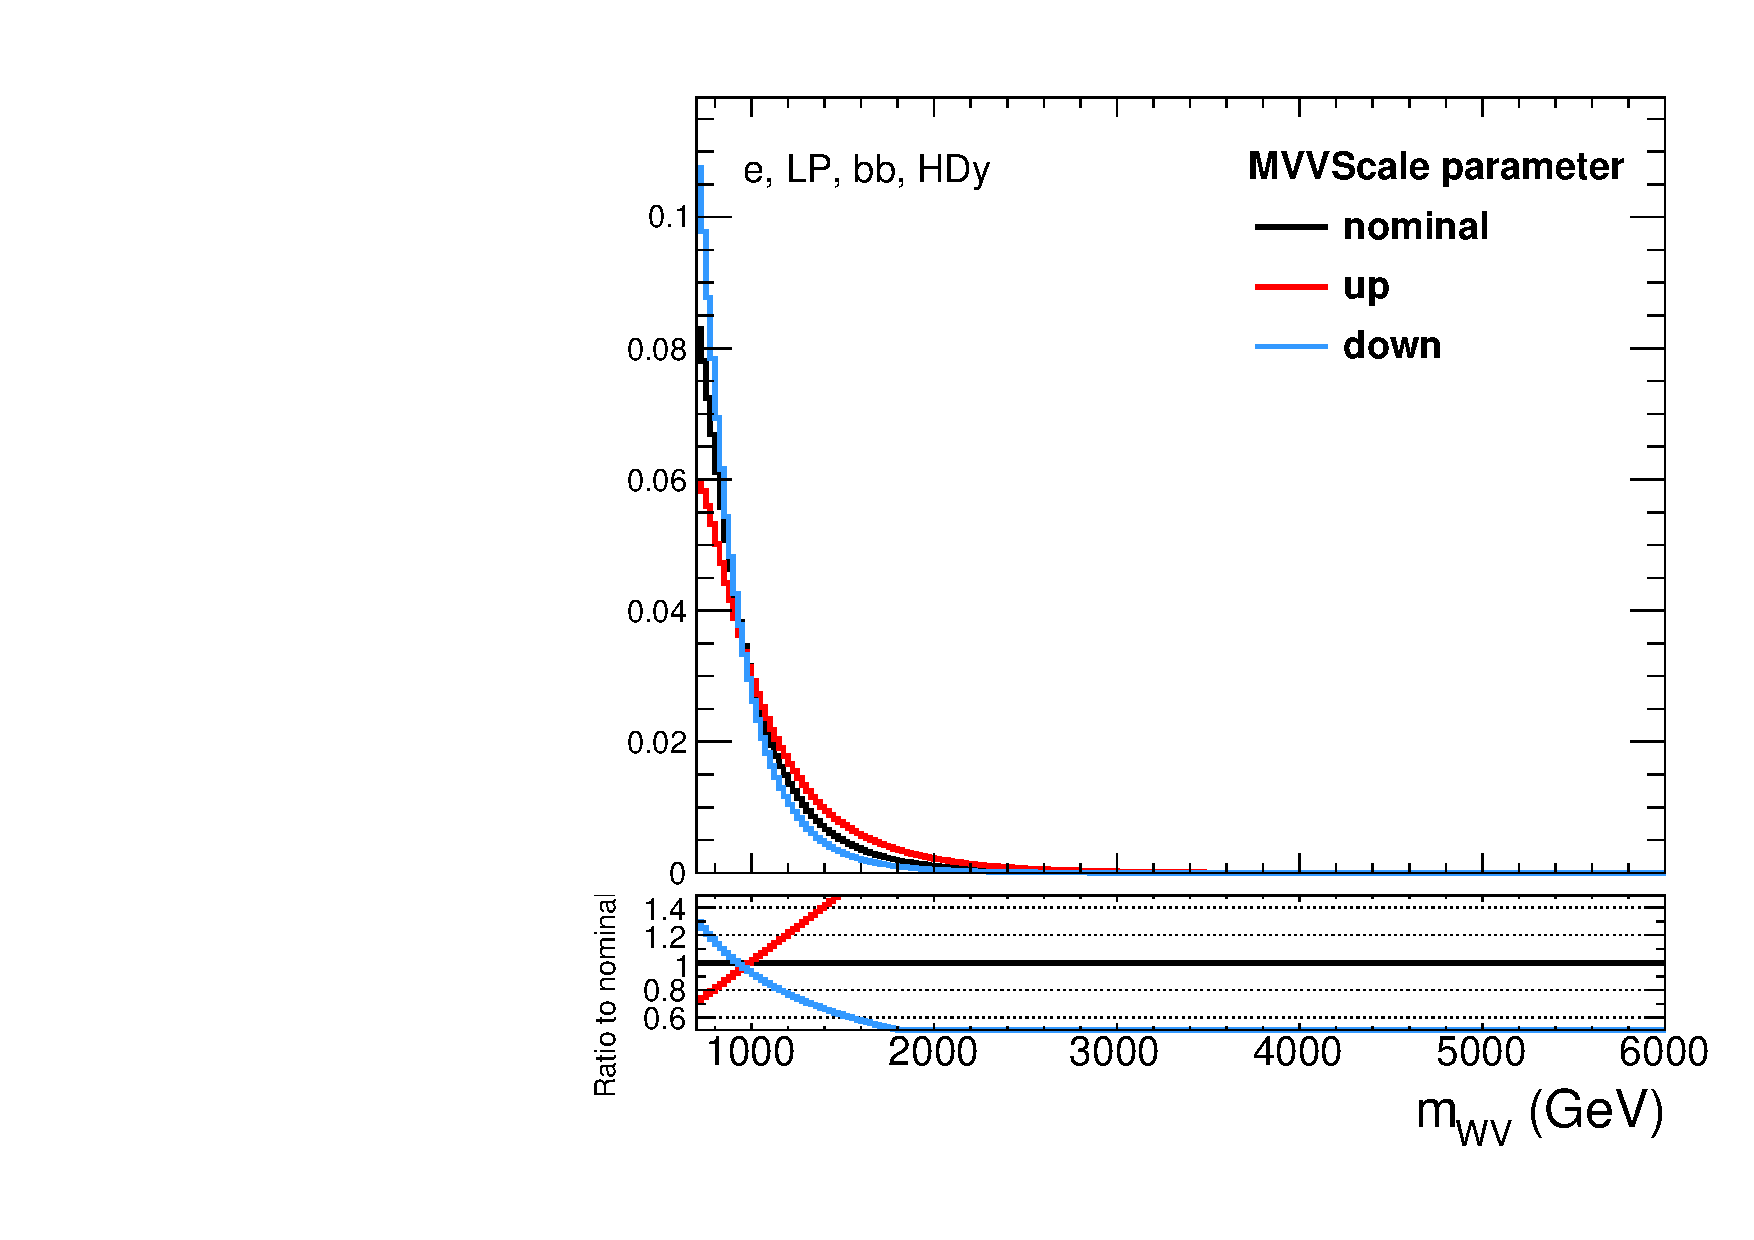
\includegraphics[width=0.21\textwidth]{fig/uncertainties/systs_nonRes_e_LP_bb_HDy_MVVScale_ProjX.pdf}\\
  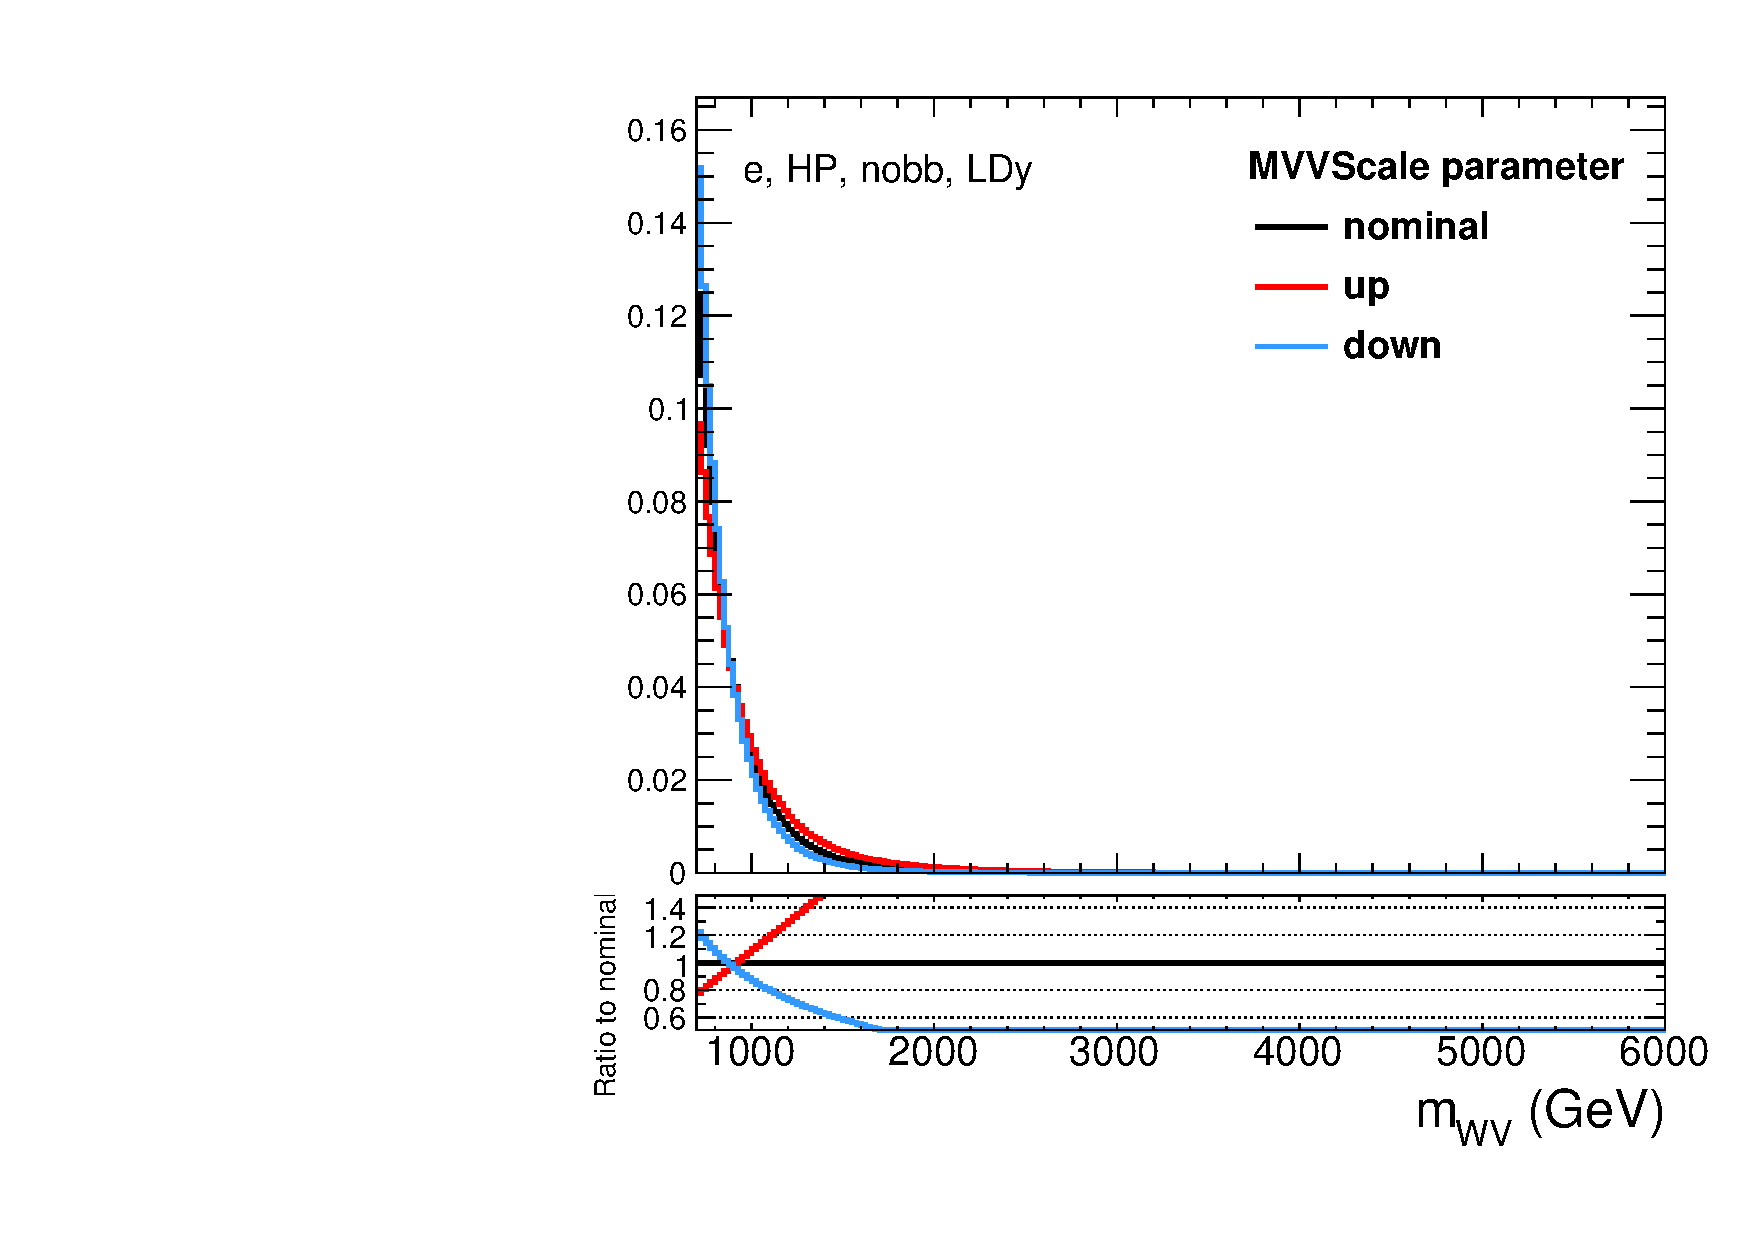
\includegraphics[width=0.21\textwidth]{fig/uncertainties/systs_nonRes_e_HP_nobb_LDy_MVVScale_ProjX.pdf}
  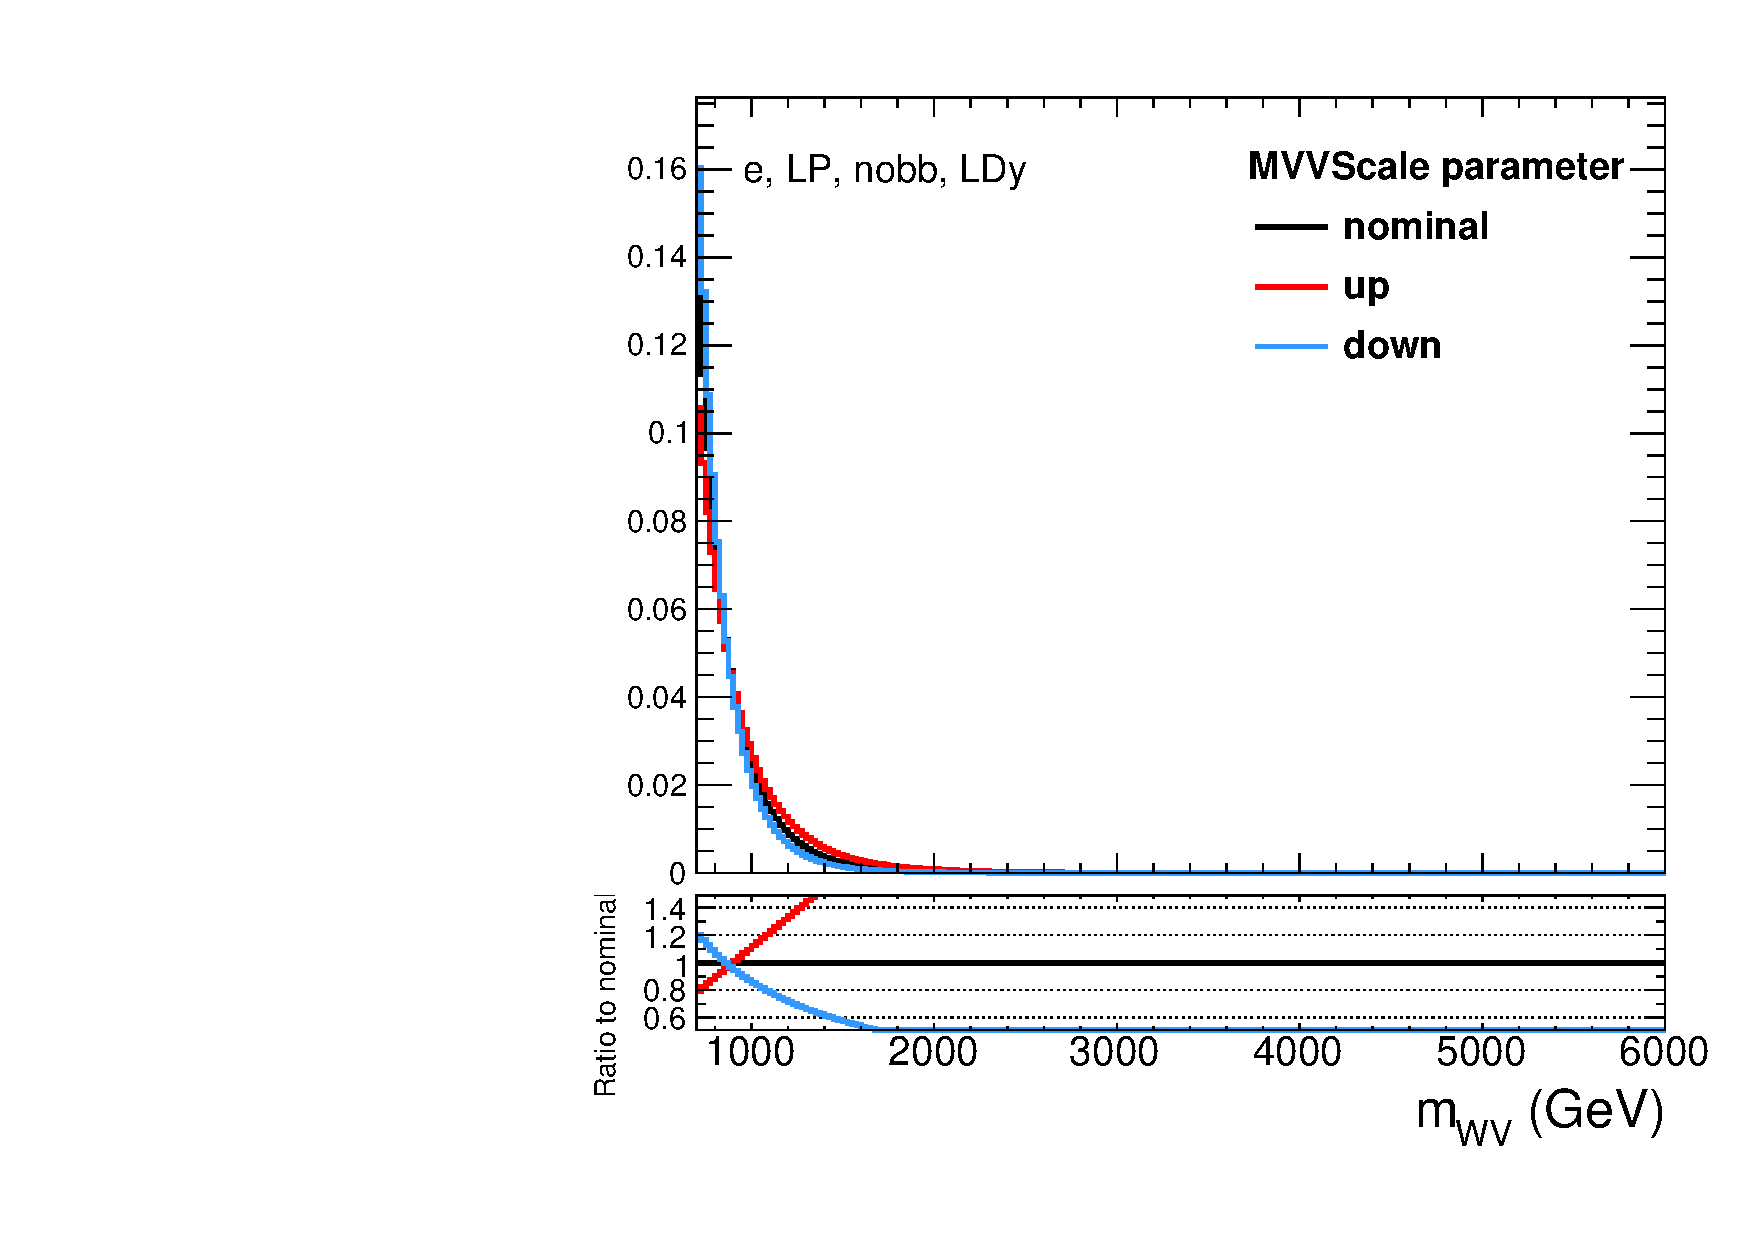
\includegraphics[width=0.21\textwidth]{fig/uncertainties/systs_nonRes_e_LP_nobb_LDy_MVVScale_ProjX.pdf}
  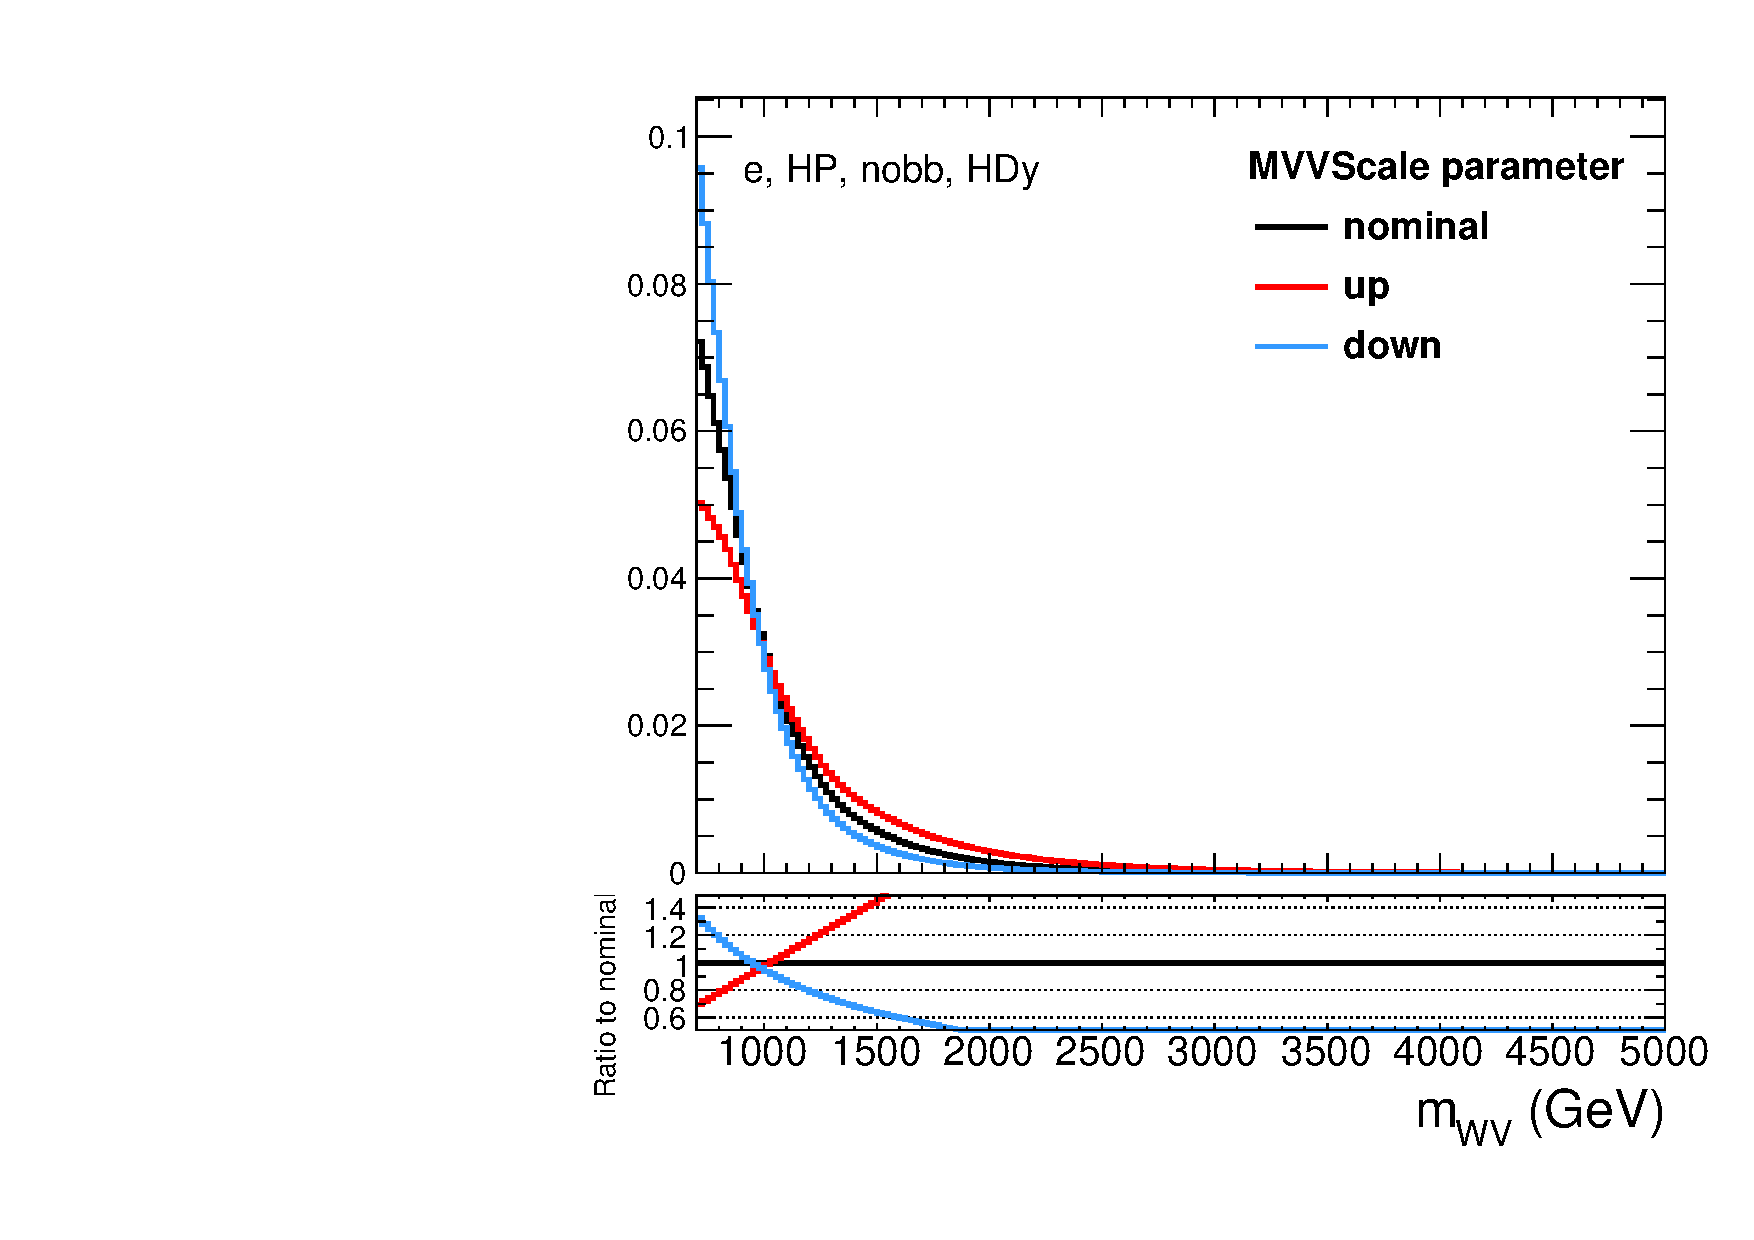
\includegraphics[width=0.21\textwidth]{fig/uncertainties/systs_nonRes_e_HP_nobb_HDy_MVVScale_ProjX.pdf}
  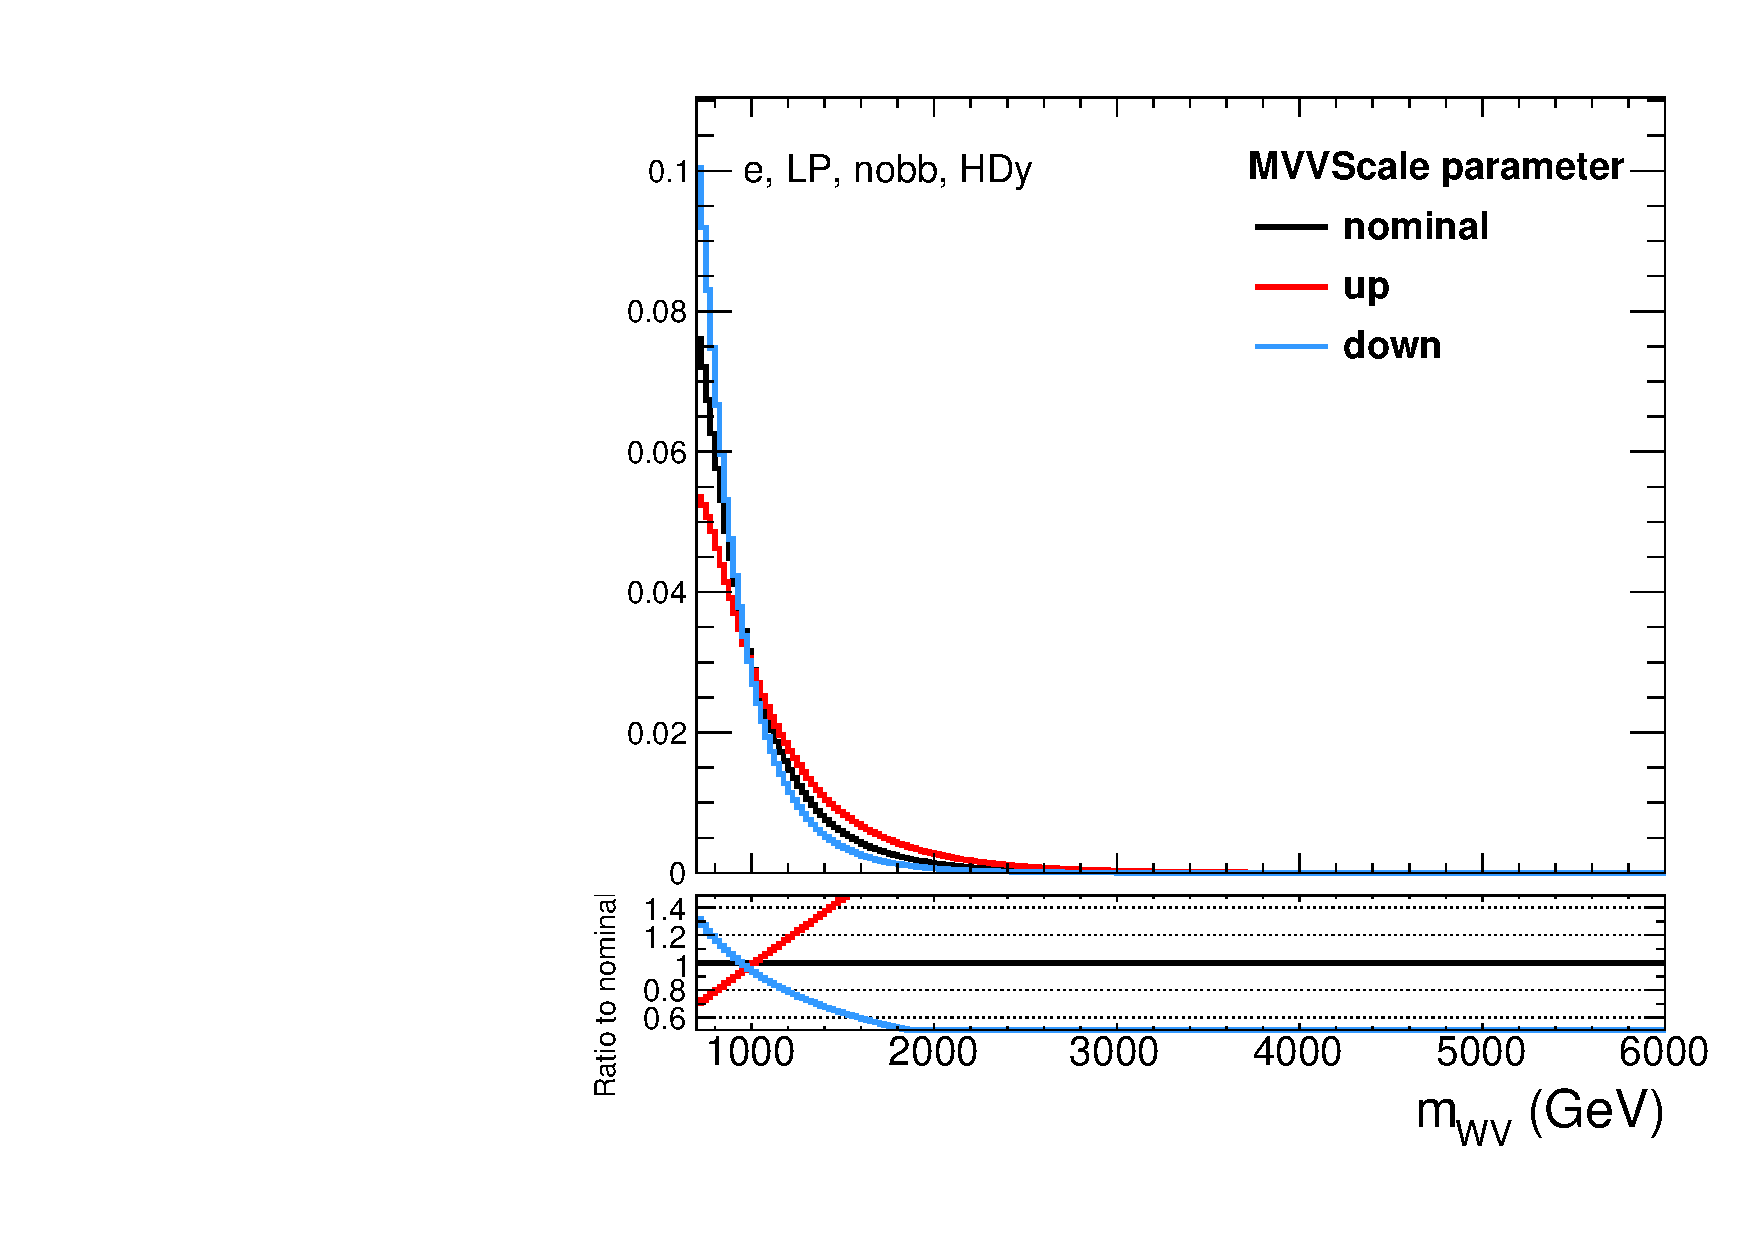
\includegraphics[width=0.21\textwidth]{fig/uncertainties/systs_nonRes_e_LP_nobb_HDy_MVVScale_ProjX.pdf}\\
  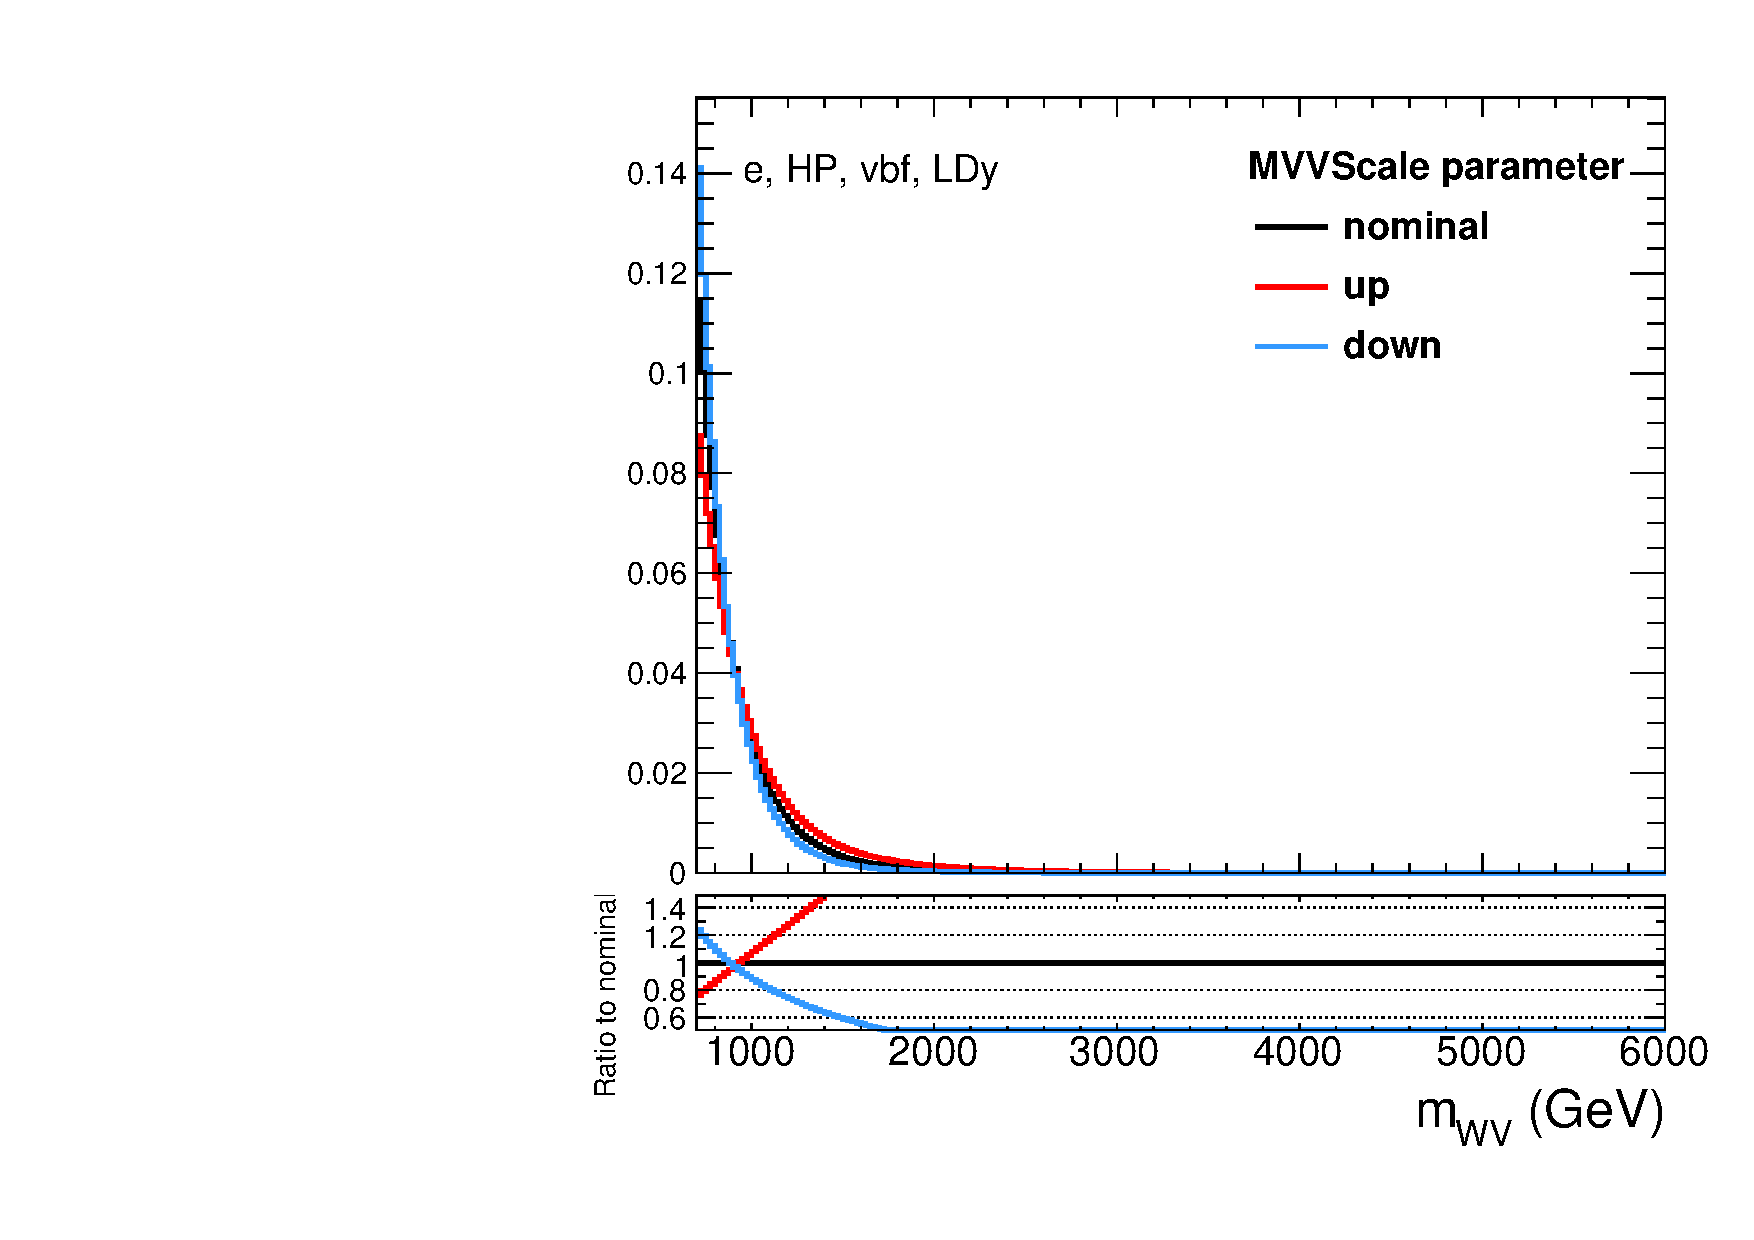
\includegraphics[width=0.21\textwidth]{fig/uncertainties/systs_nonRes_e_HP_vbf_LDy_MVVScale_ProjX.pdf}
  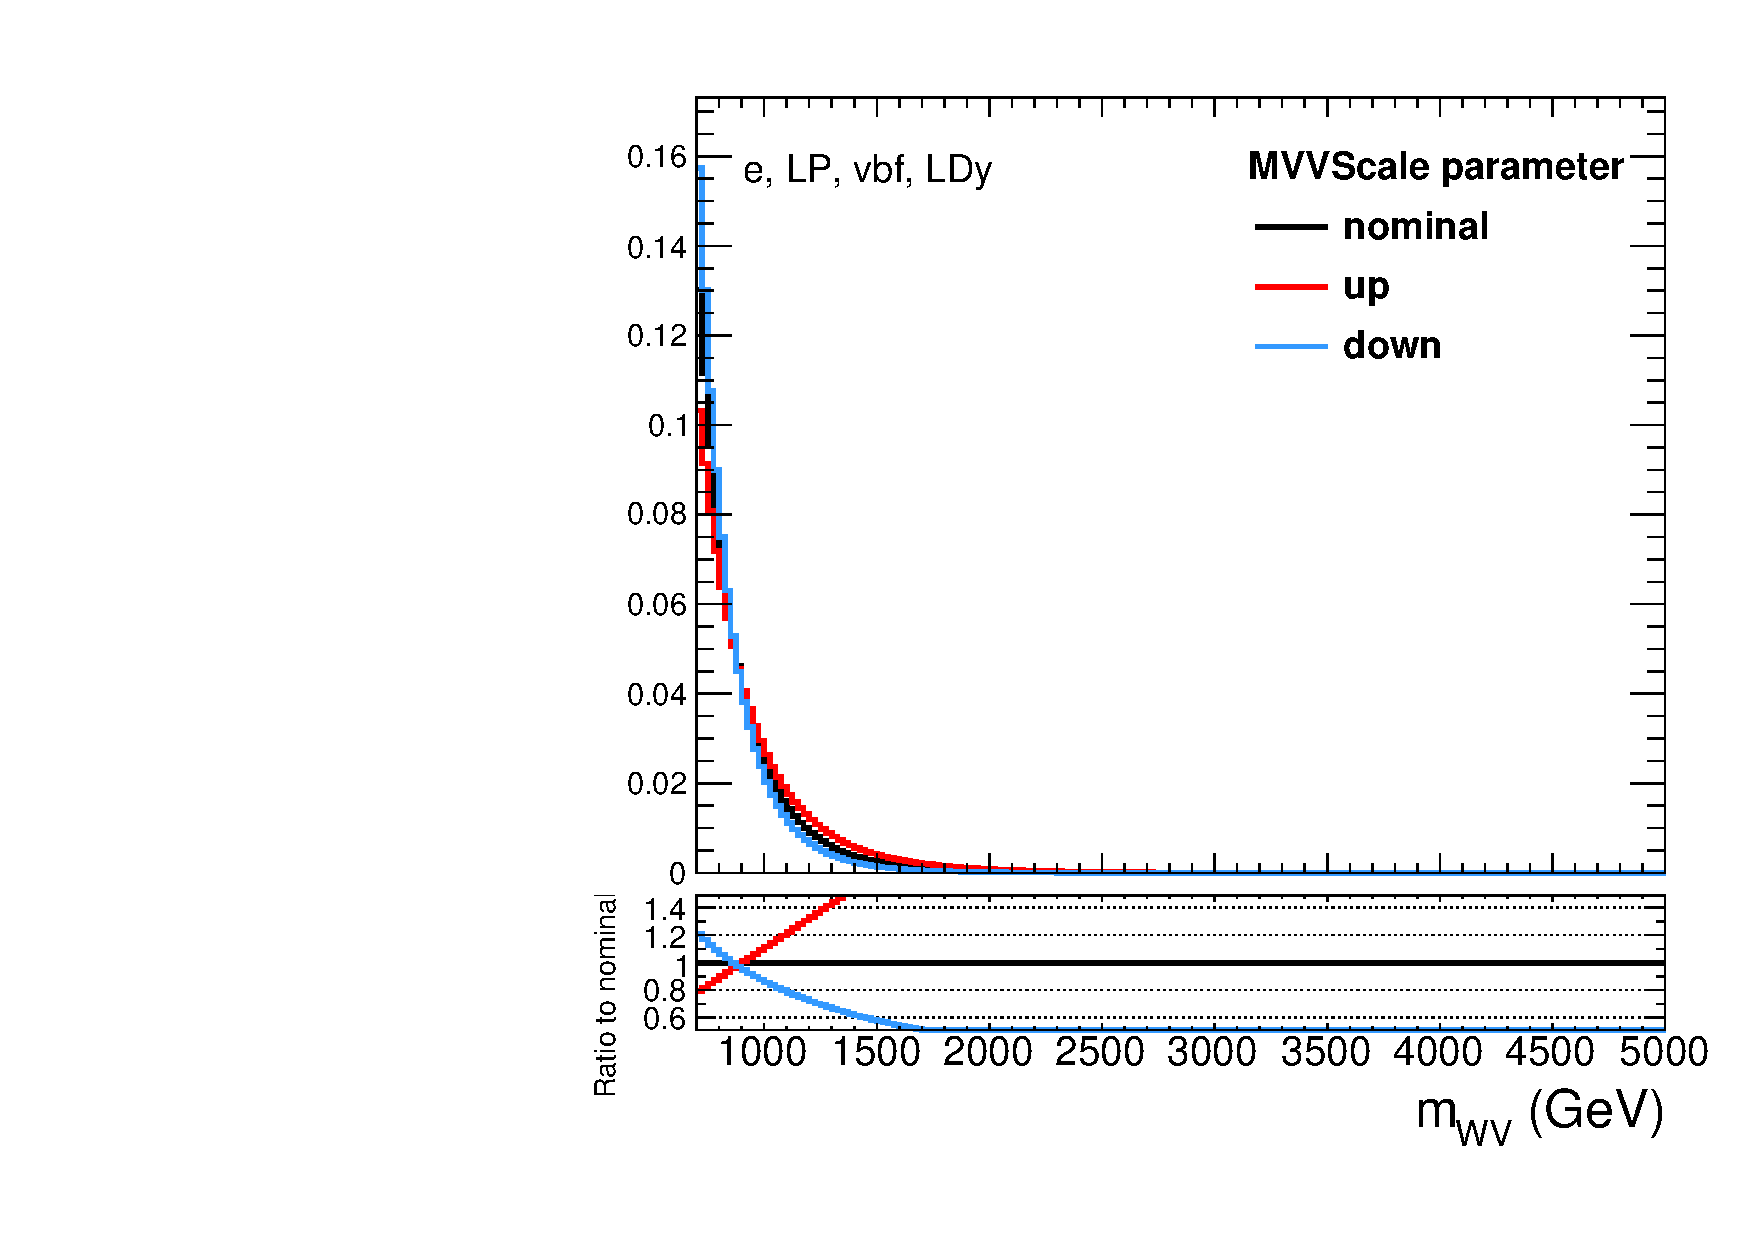
\includegraphics[width=0.21\textwidth]{fig/uncertainties/systs_nonRes_e_LP_vbf_LDy_MVVScale_ProjX.pdf}
  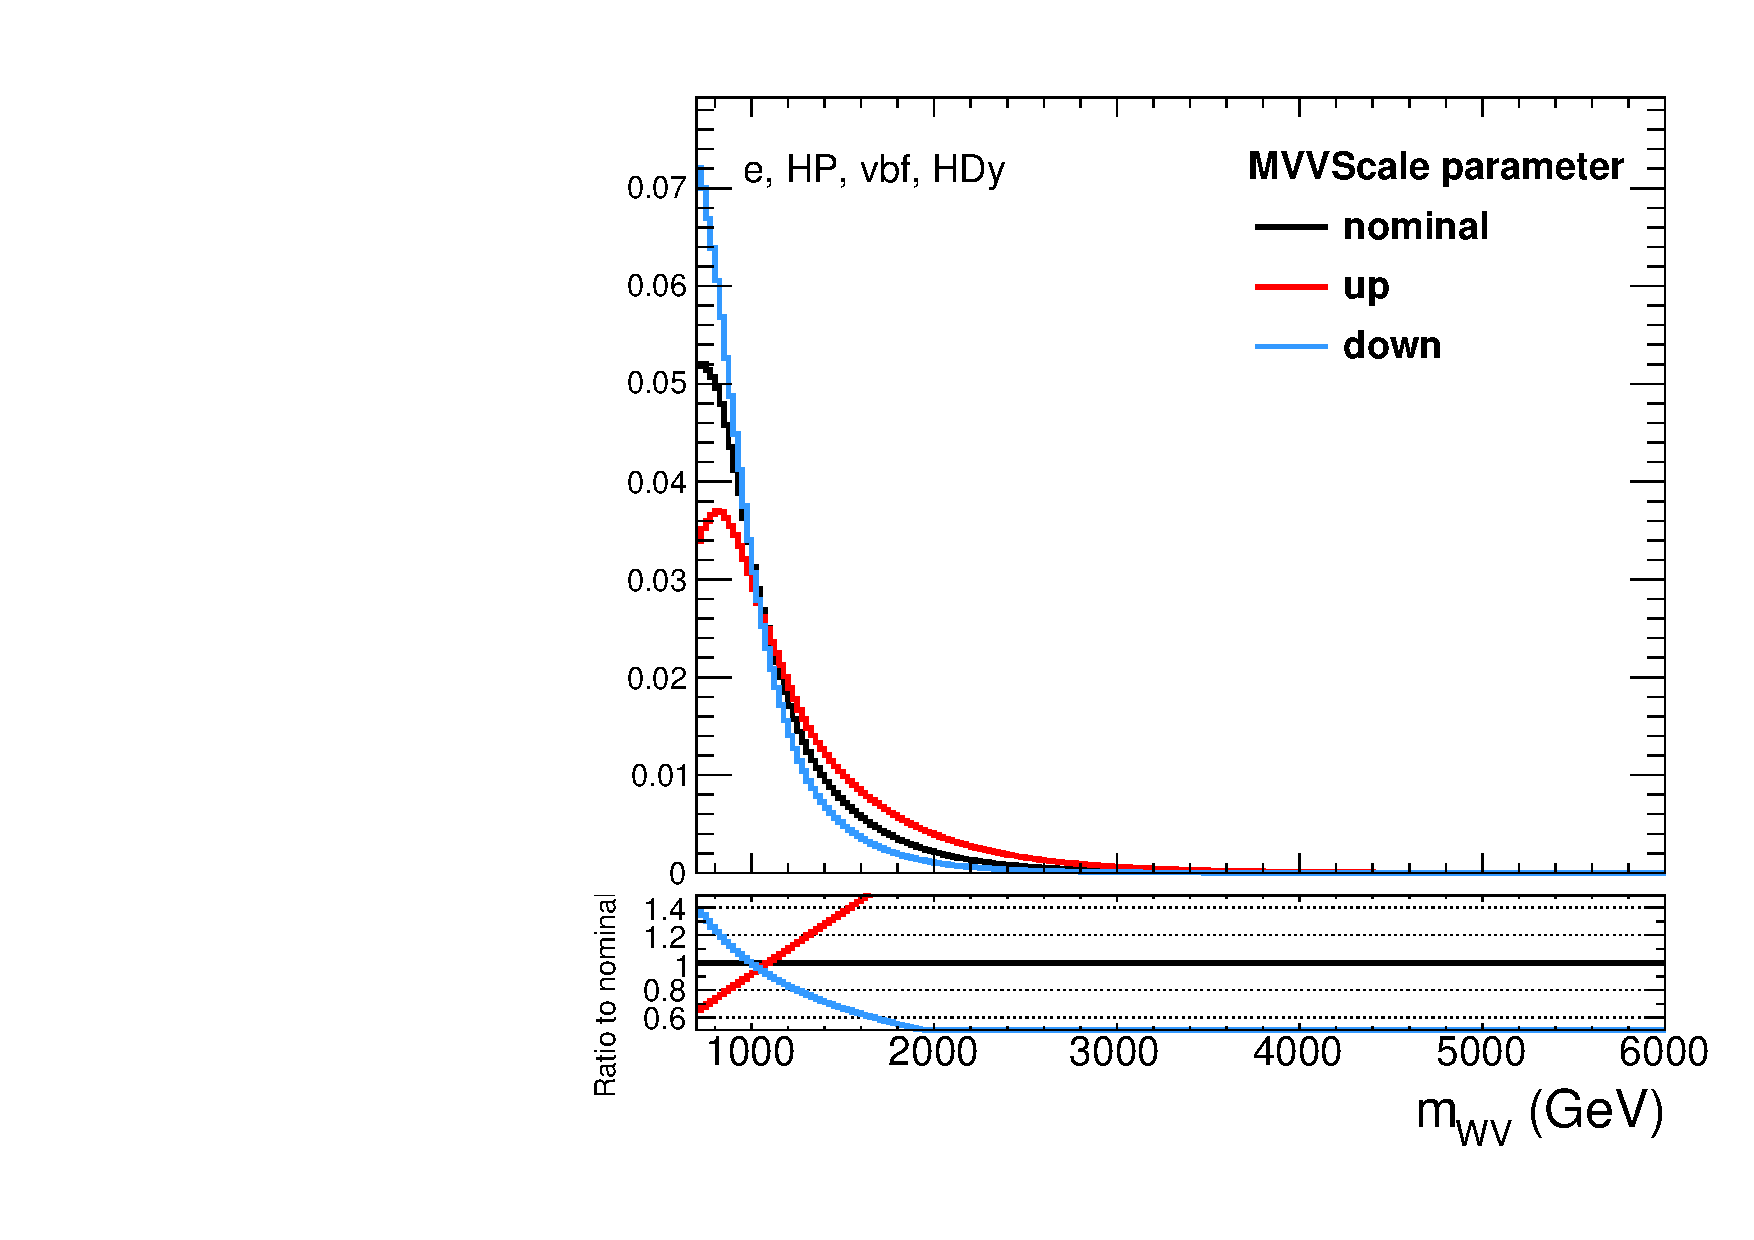
\includegraphics[width=0.21\textwidth]{fig/uncertainties/systs_nonRes_e_HP_vbf_HDy_MVVScale_ProjX.pdf}
  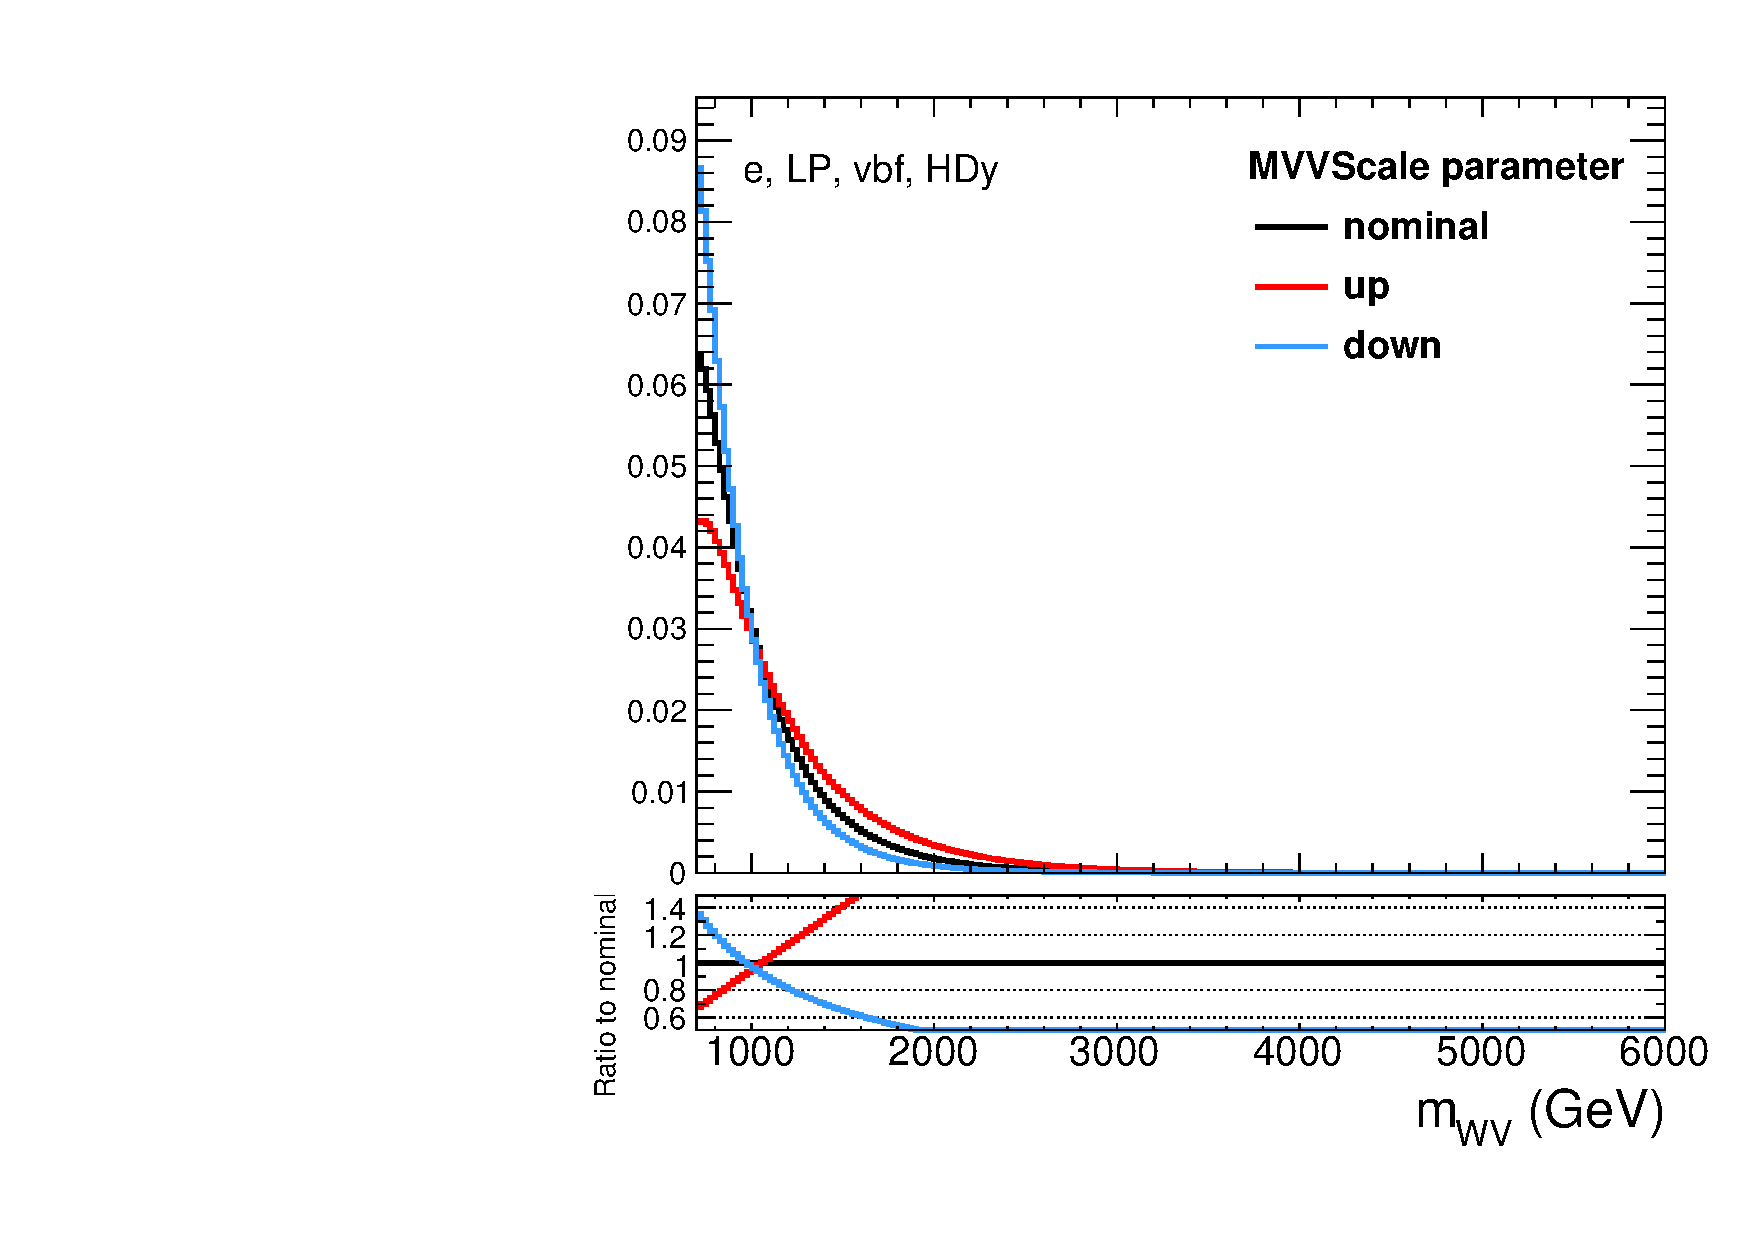
\includegraphics[width=0.21\textwidth]{fig/uncertainties/systs_nonRes_e_LP_vbf_HDy_MVVScale_ProjX.pdf}\\
  \caption{
    Projections of the nominal and alternative shapes of the non-resonant background onto the \MVV dimension obtained from applying $\pm3\sigma$ variations of the jet \pt spectrum uncertainties for the electron channel.
    Columns 1 to 4: HP-LDy, LP-LDy, HP-HDy, LP-HDy.
    Rows 1 to 3: bb, nobb, vbf.
  }
  \label{fig:systNonResMVV_MVVScale}
\end{figure}

\begin{figure}[htbp]
  \centering
  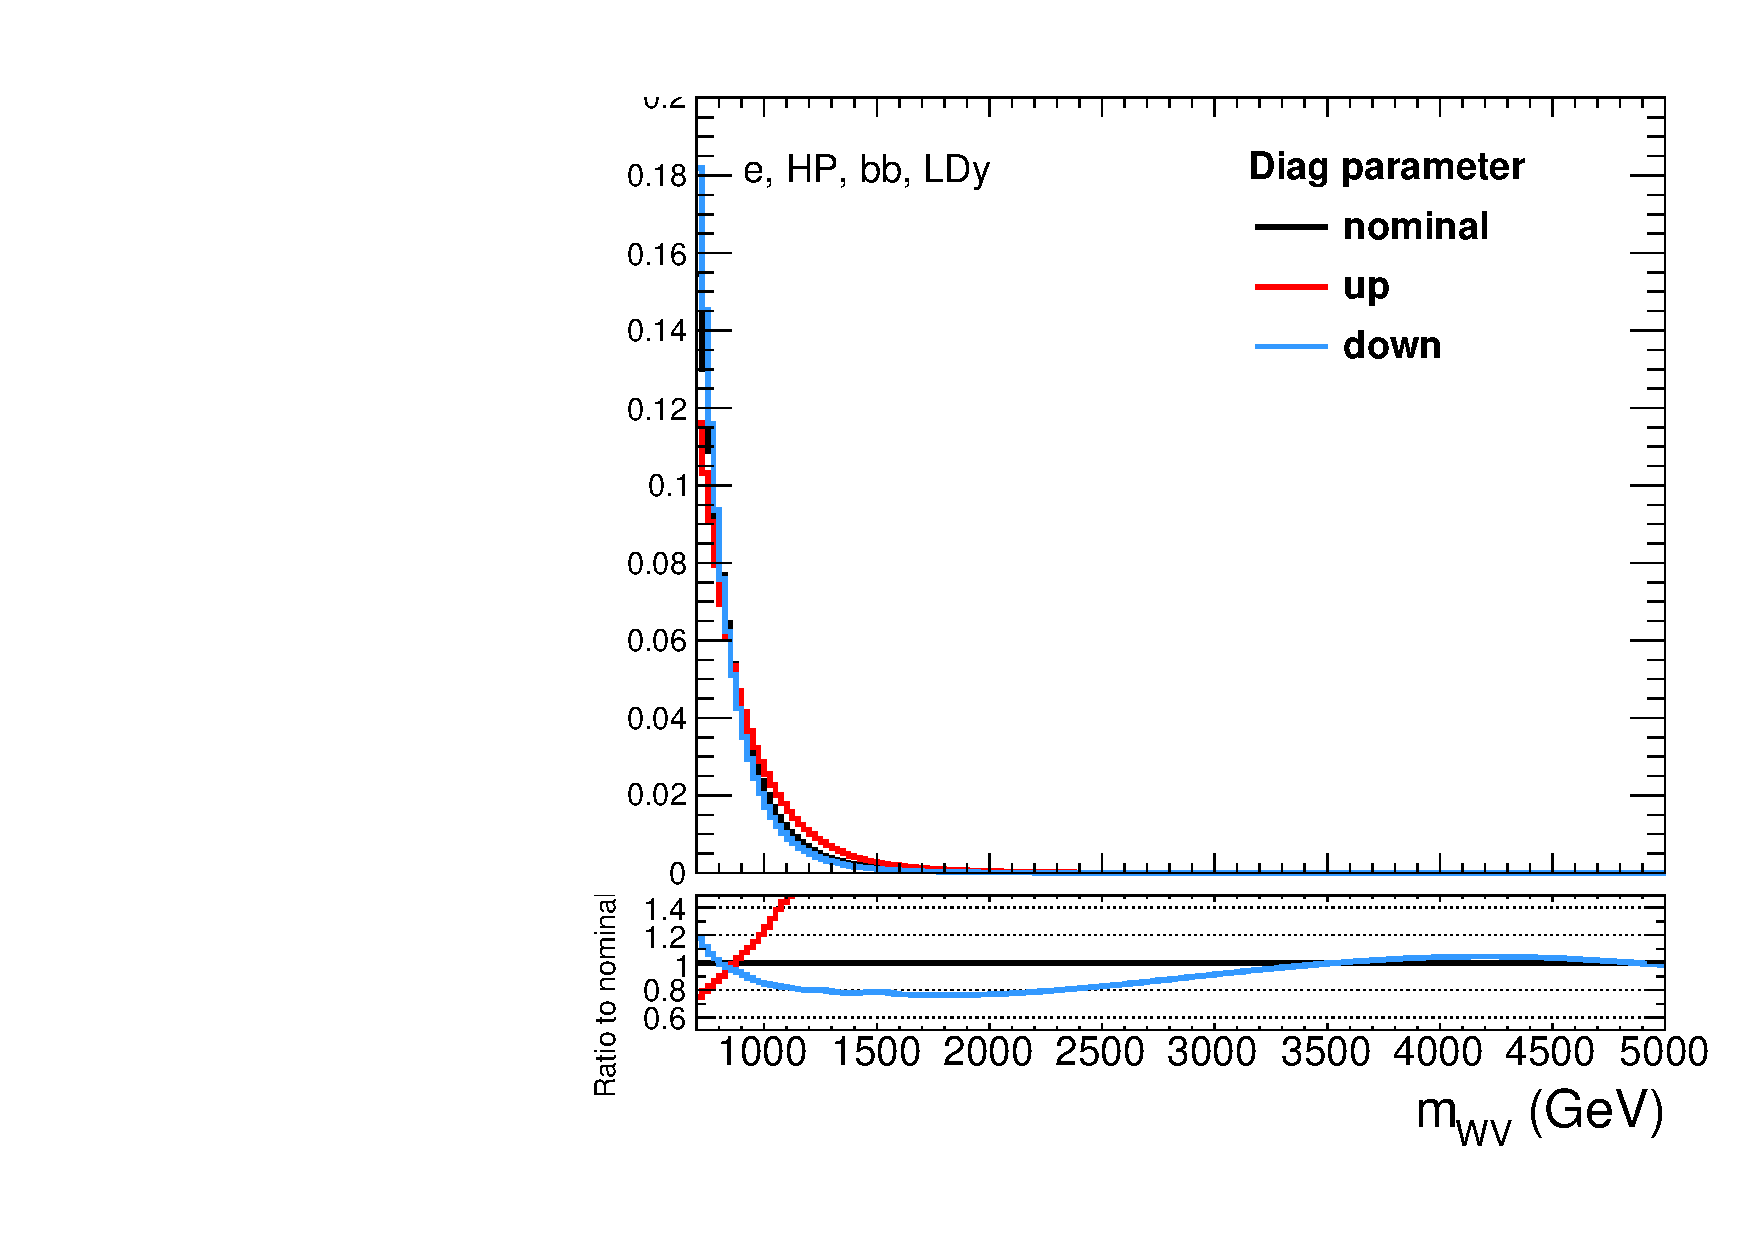
\includegraphics[width=0.21\textwidth]{fig/uncertainties/systs_nonRes_e_HP_bb_LDy_Diag_ProjX.pdf}
  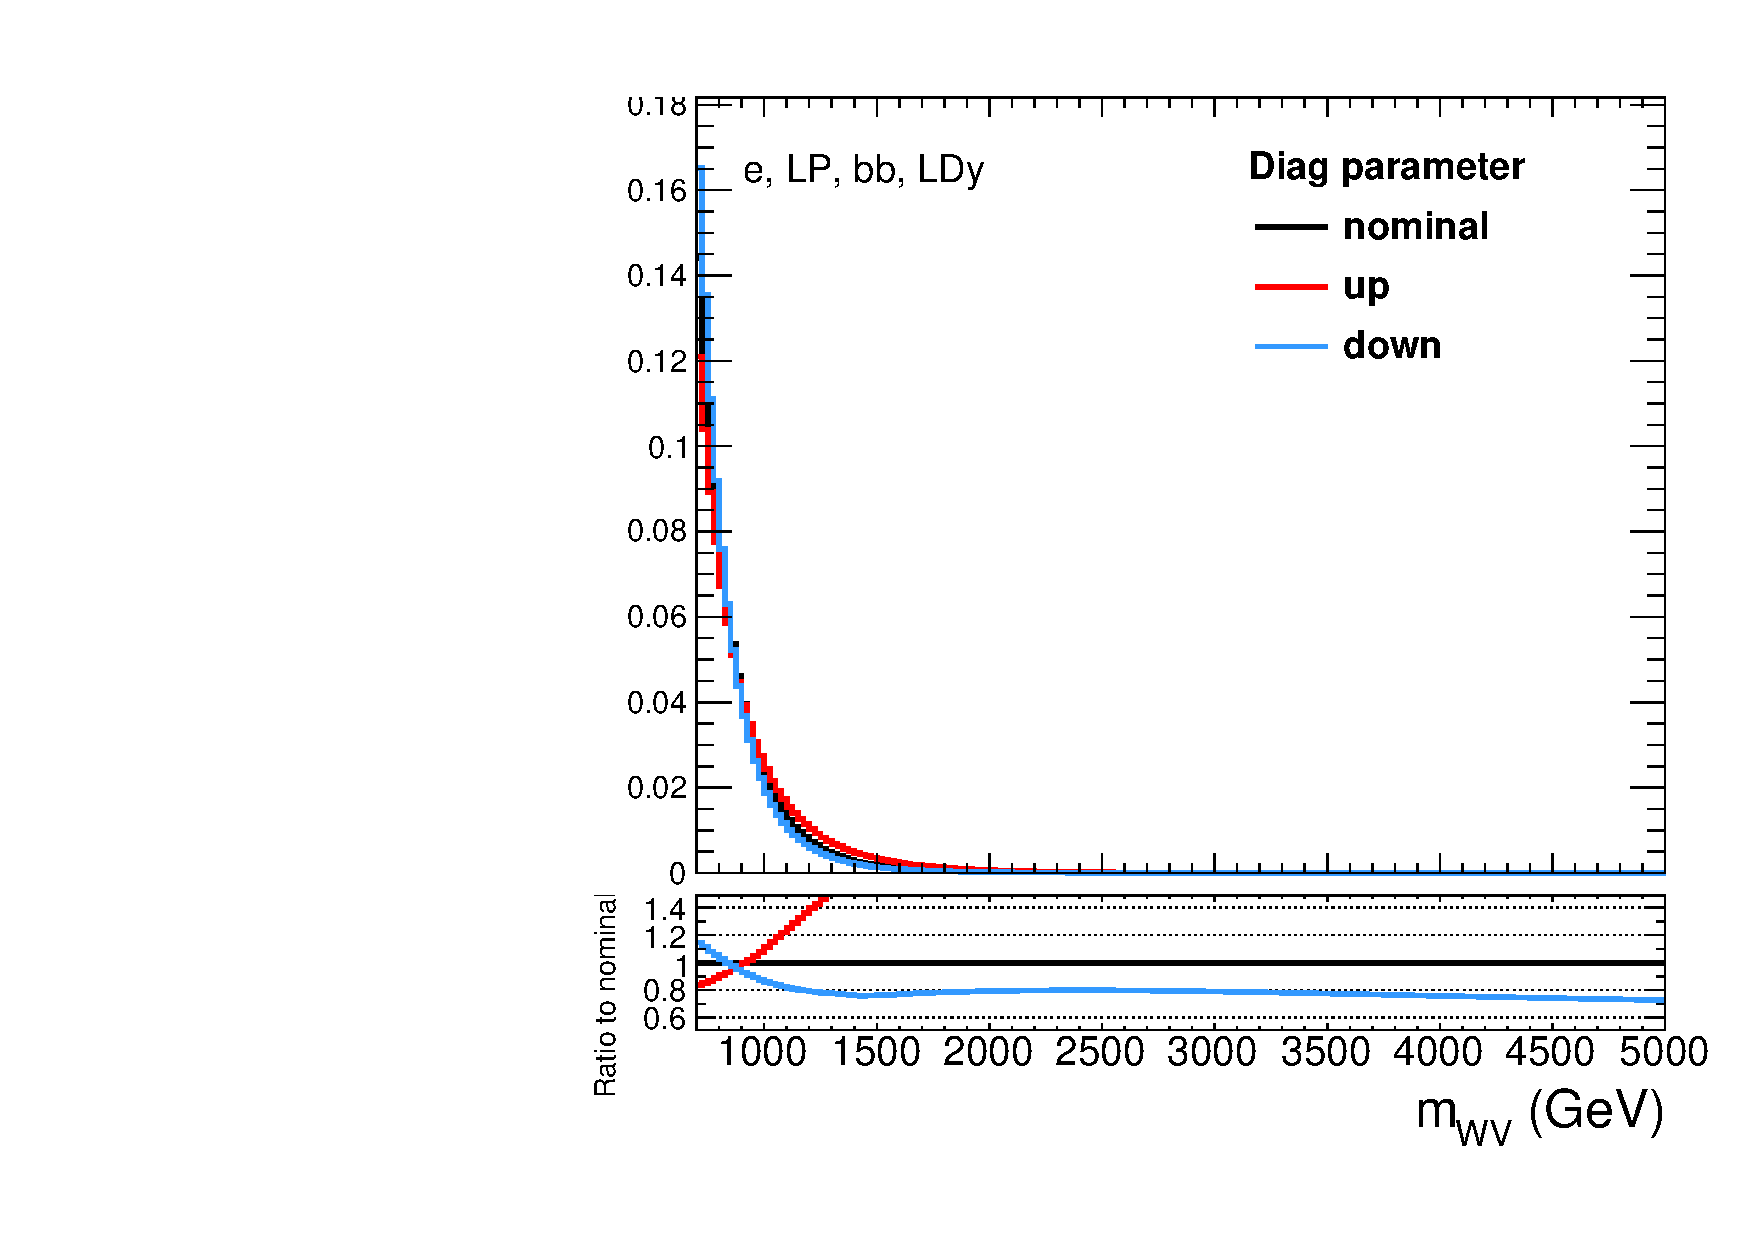
\includegraphics[width=0.21\textwidth]{fig/uncertainties/systs_nonRes_e_LP_bb_LDy_Diag_ProjX.pdf}
  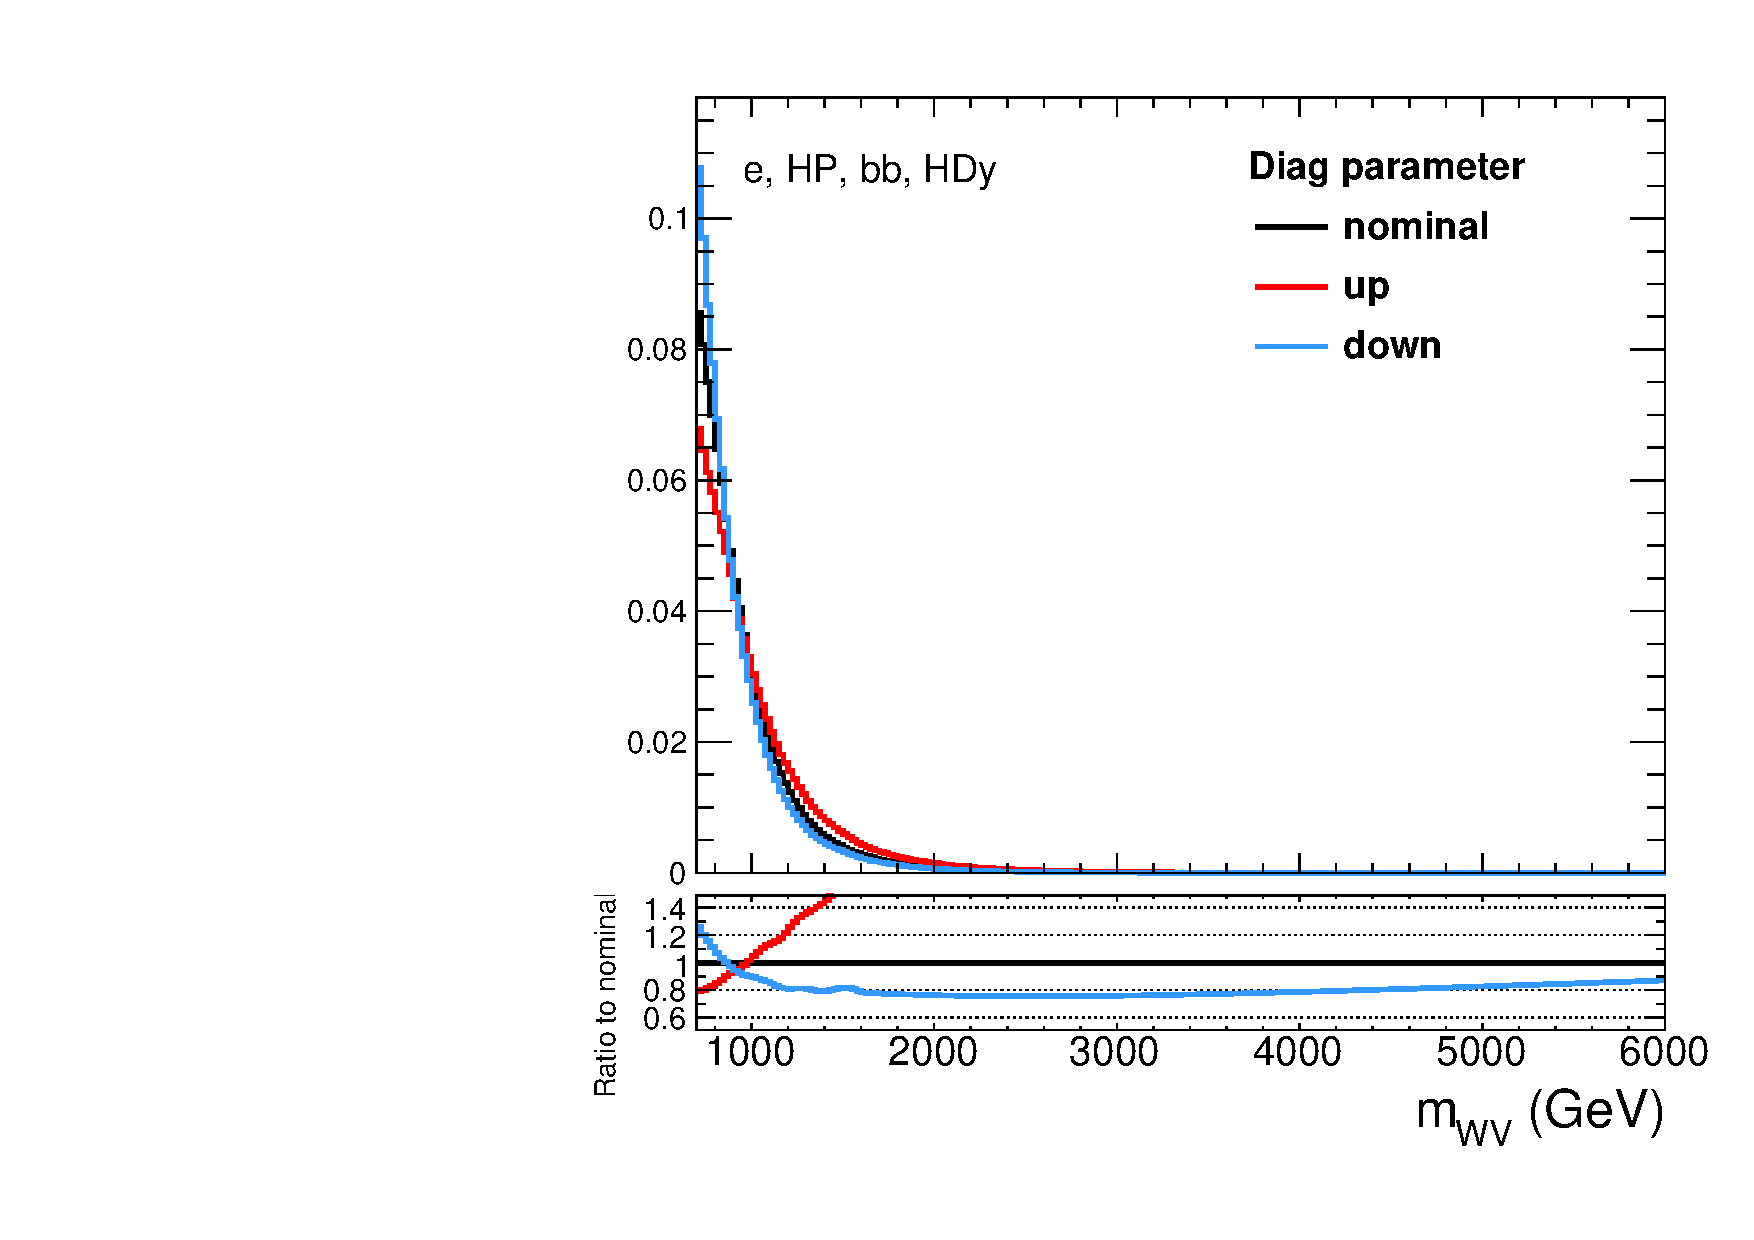
\includegraphics[width=0.21\textwidth]{fig/uncertainties/systs_nonRes_e_HP_bb_HDy_Diag_ProjX.pdf}
  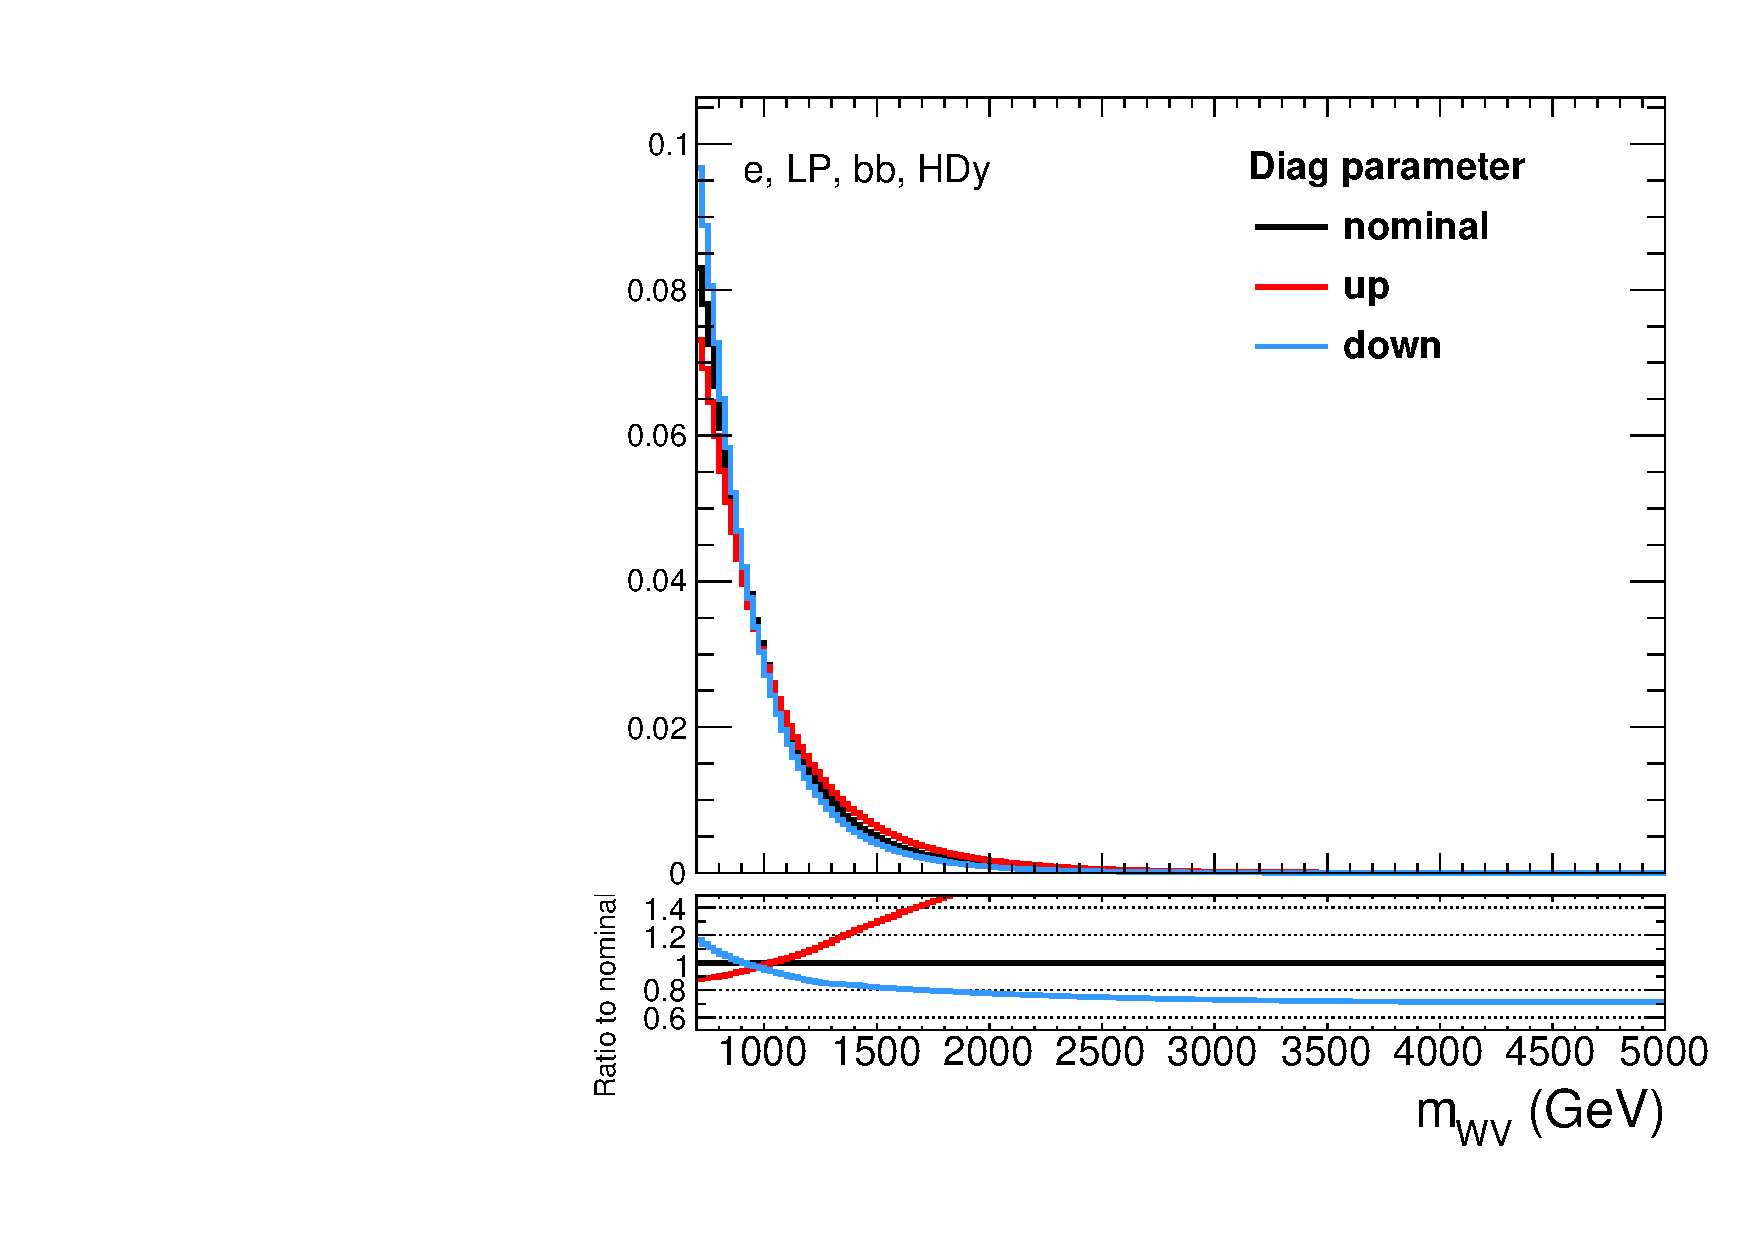
\includegraphics[width=0.21\textwidth]{fig/uncertainties/systs_nonRes_e_LP_bb_HDy_Diag_ProjX.pdf}\\
  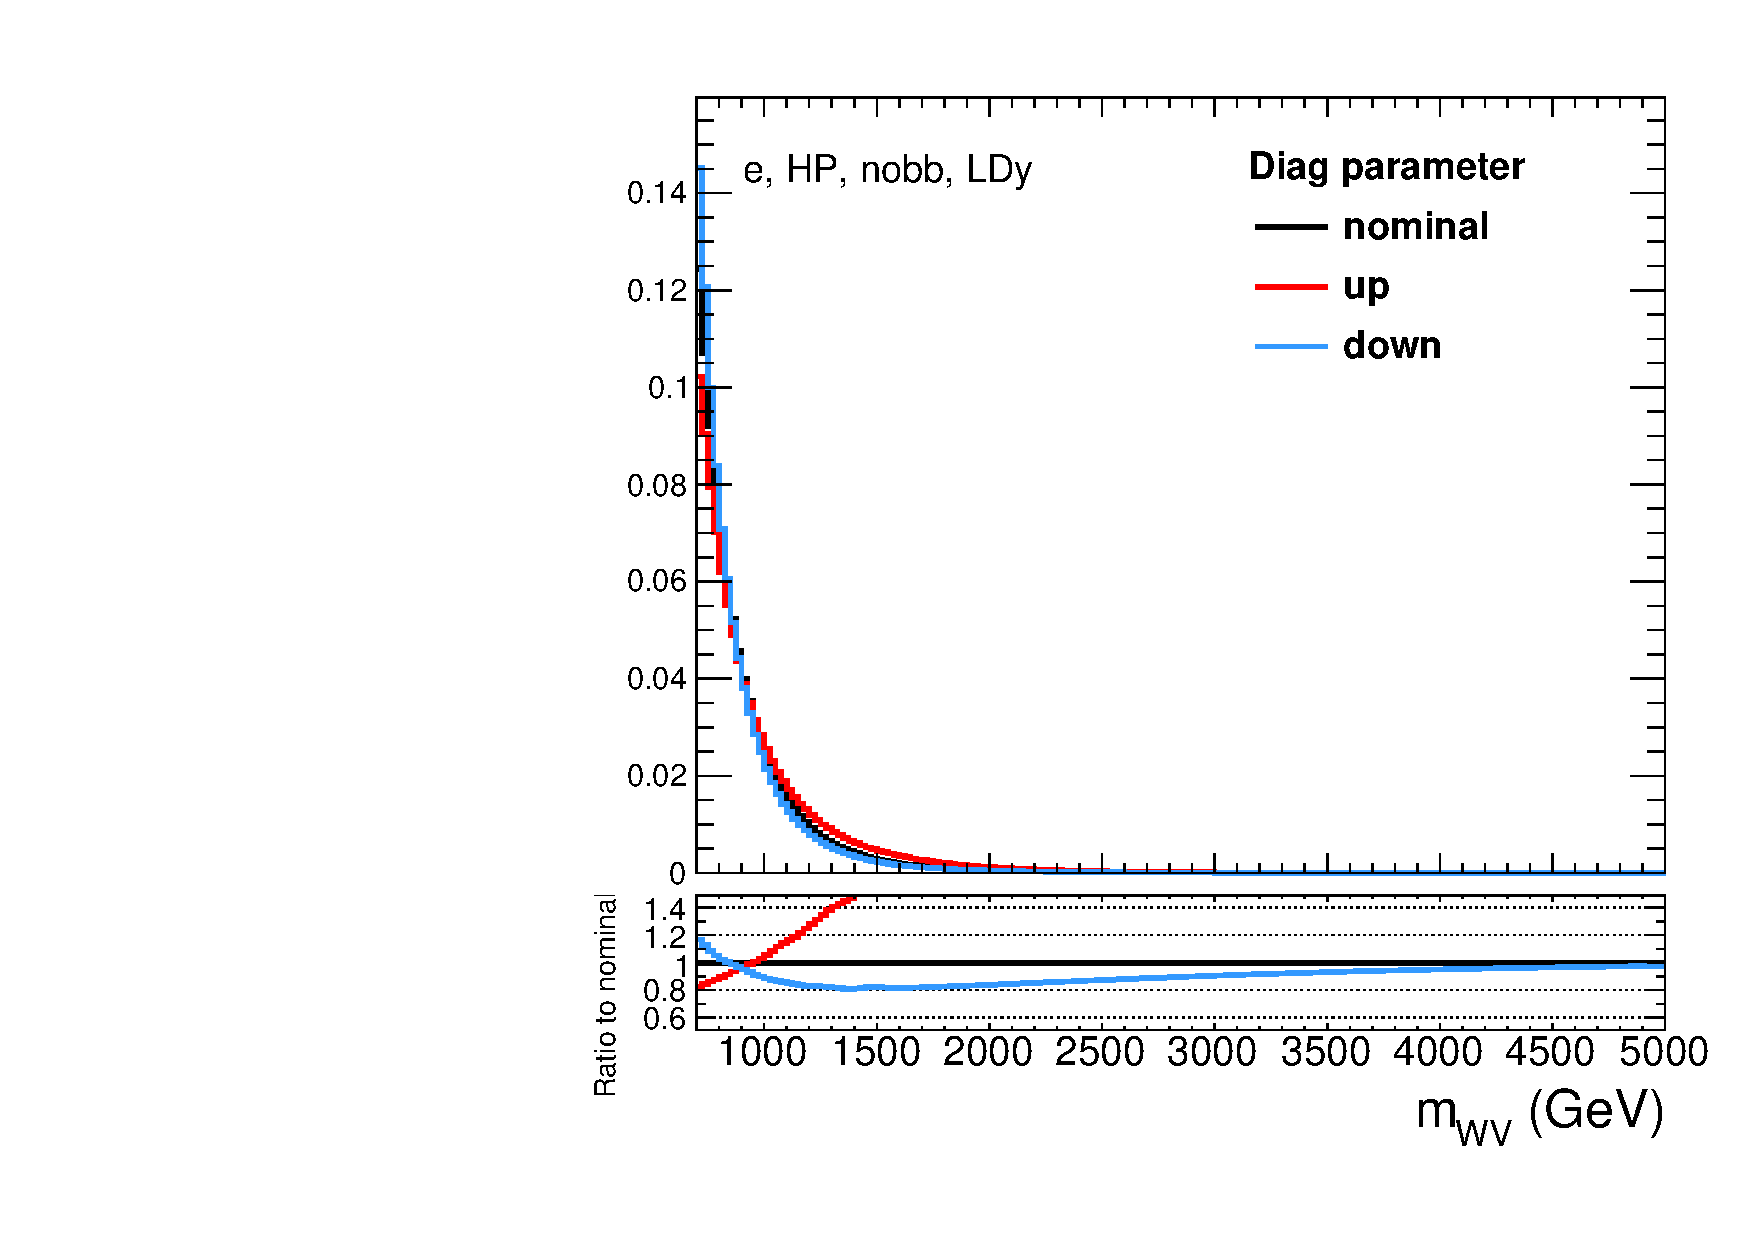
\includegraphics[width=0.21\textwidth]{fig/uncertainties/systs_nonRes_e_HP_nobb_LDy_Diag_ProjX.pdf}
  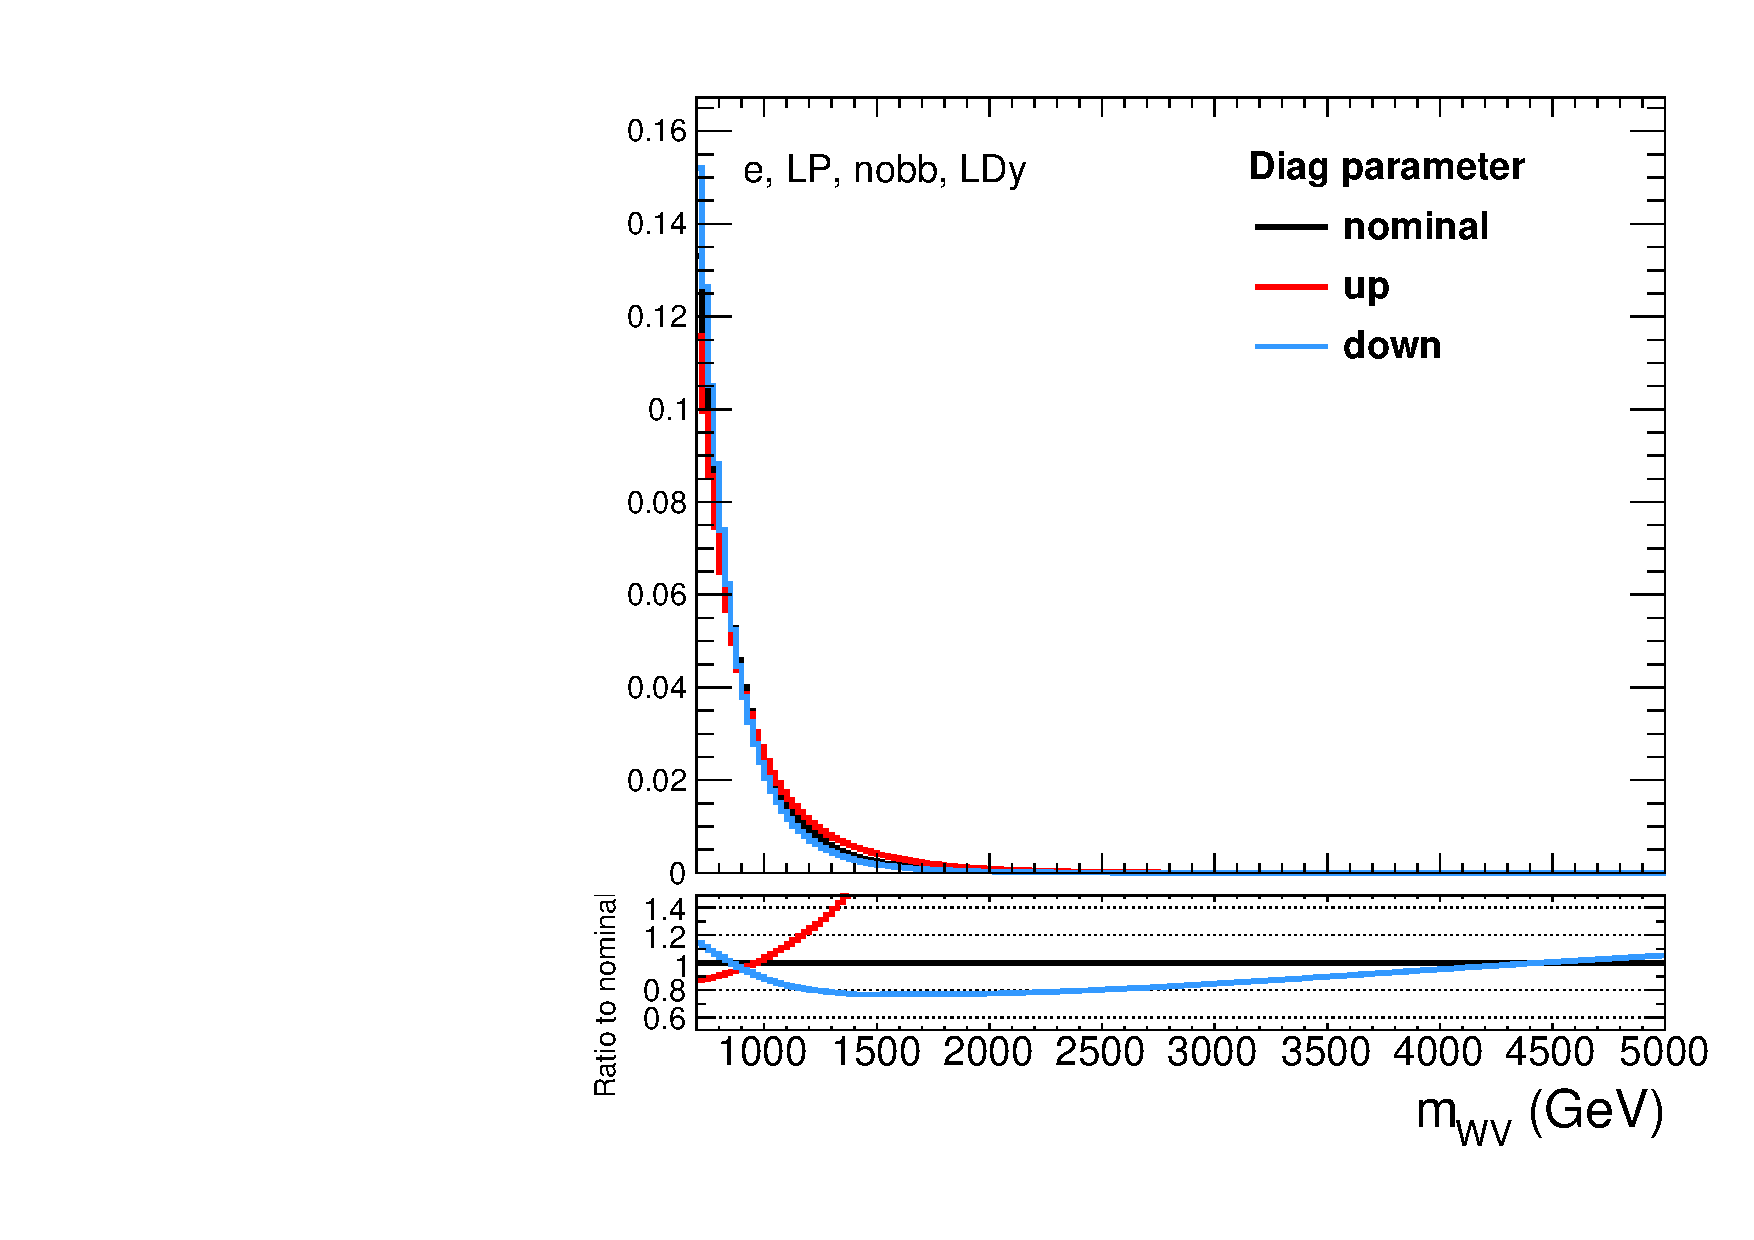
\includegraphics[width=0.21\textwidth]{fig/uncertainties/systs_nonRes_e_LP_nobb_LDy_Diag_ProjX.pdf}
  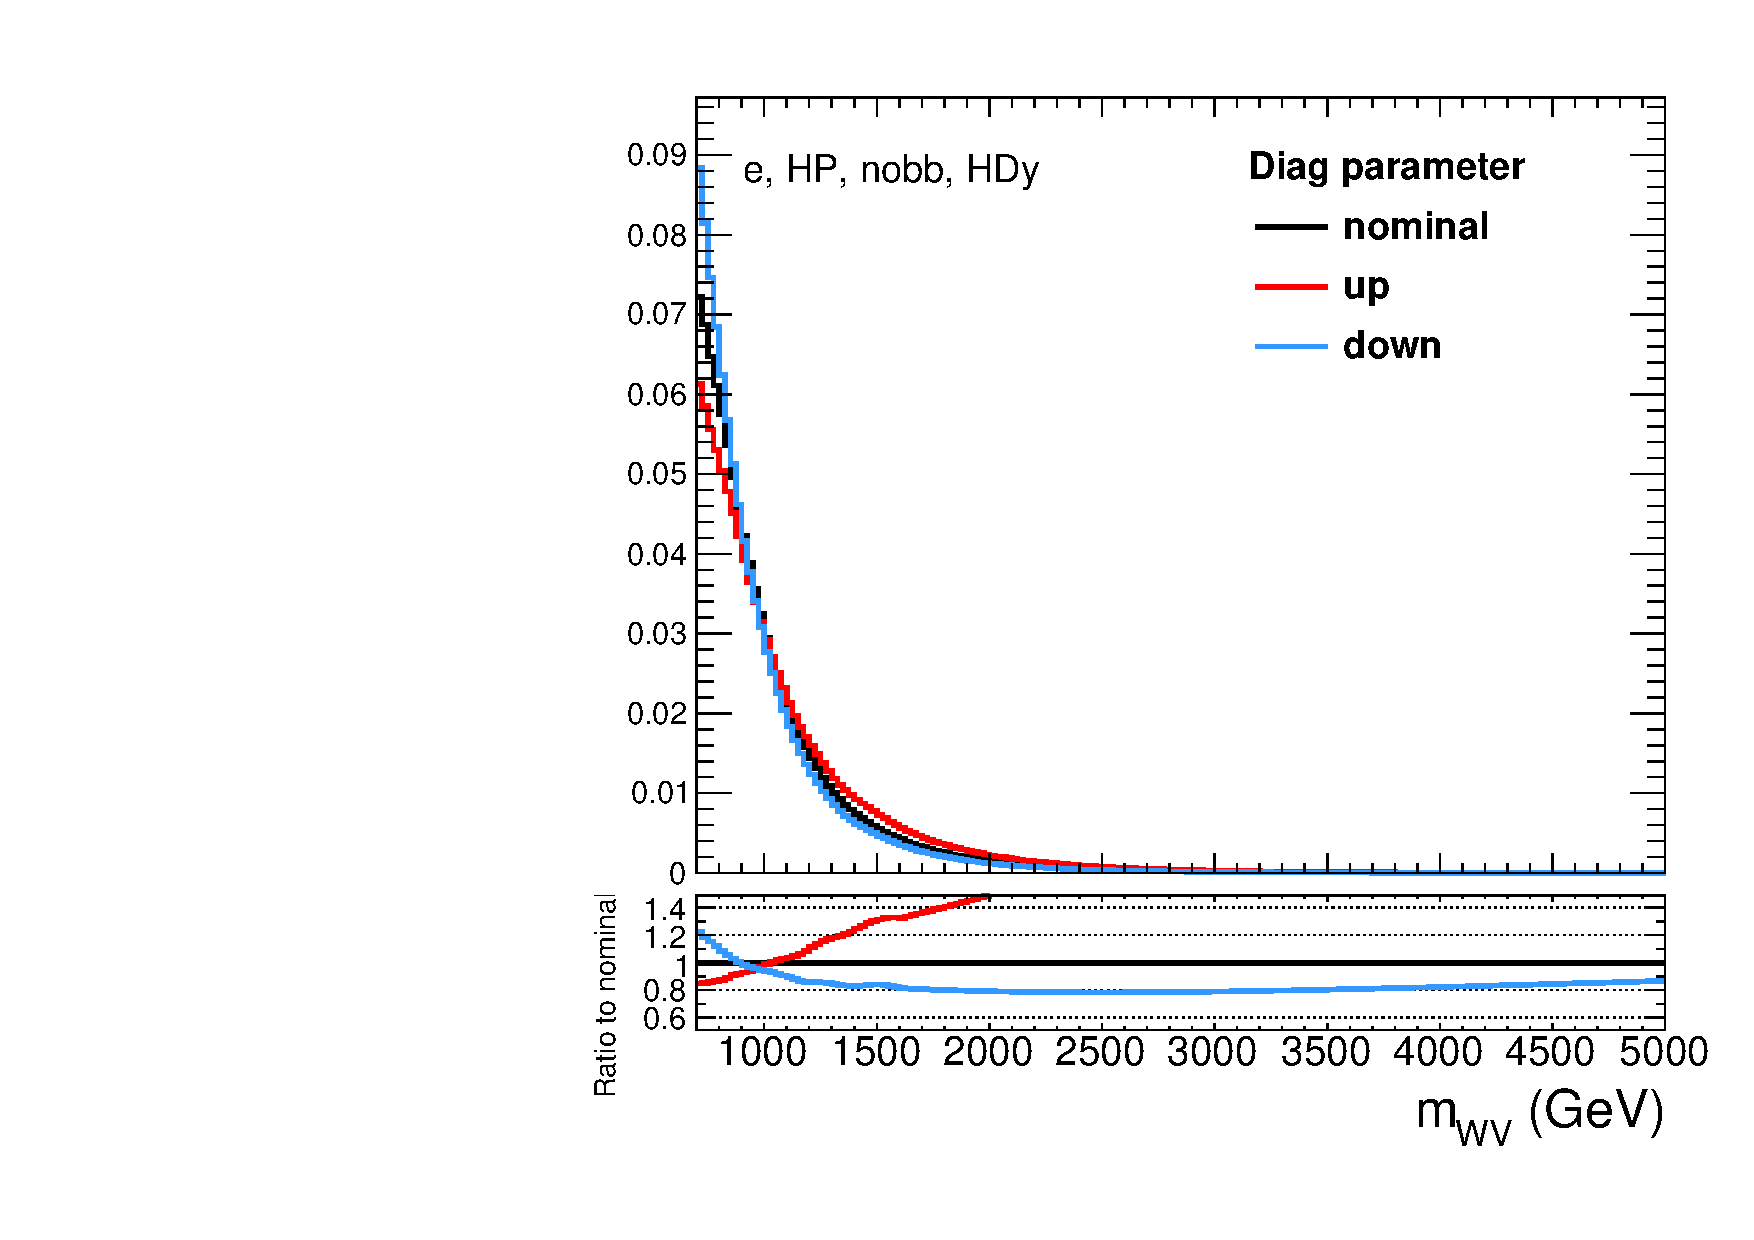
\includegraphics[width=0.21\textwidth]{fig/uncertainties/systs_nonRes_e_HP_nobb_HDy_Diag_ProjX.pdf}
  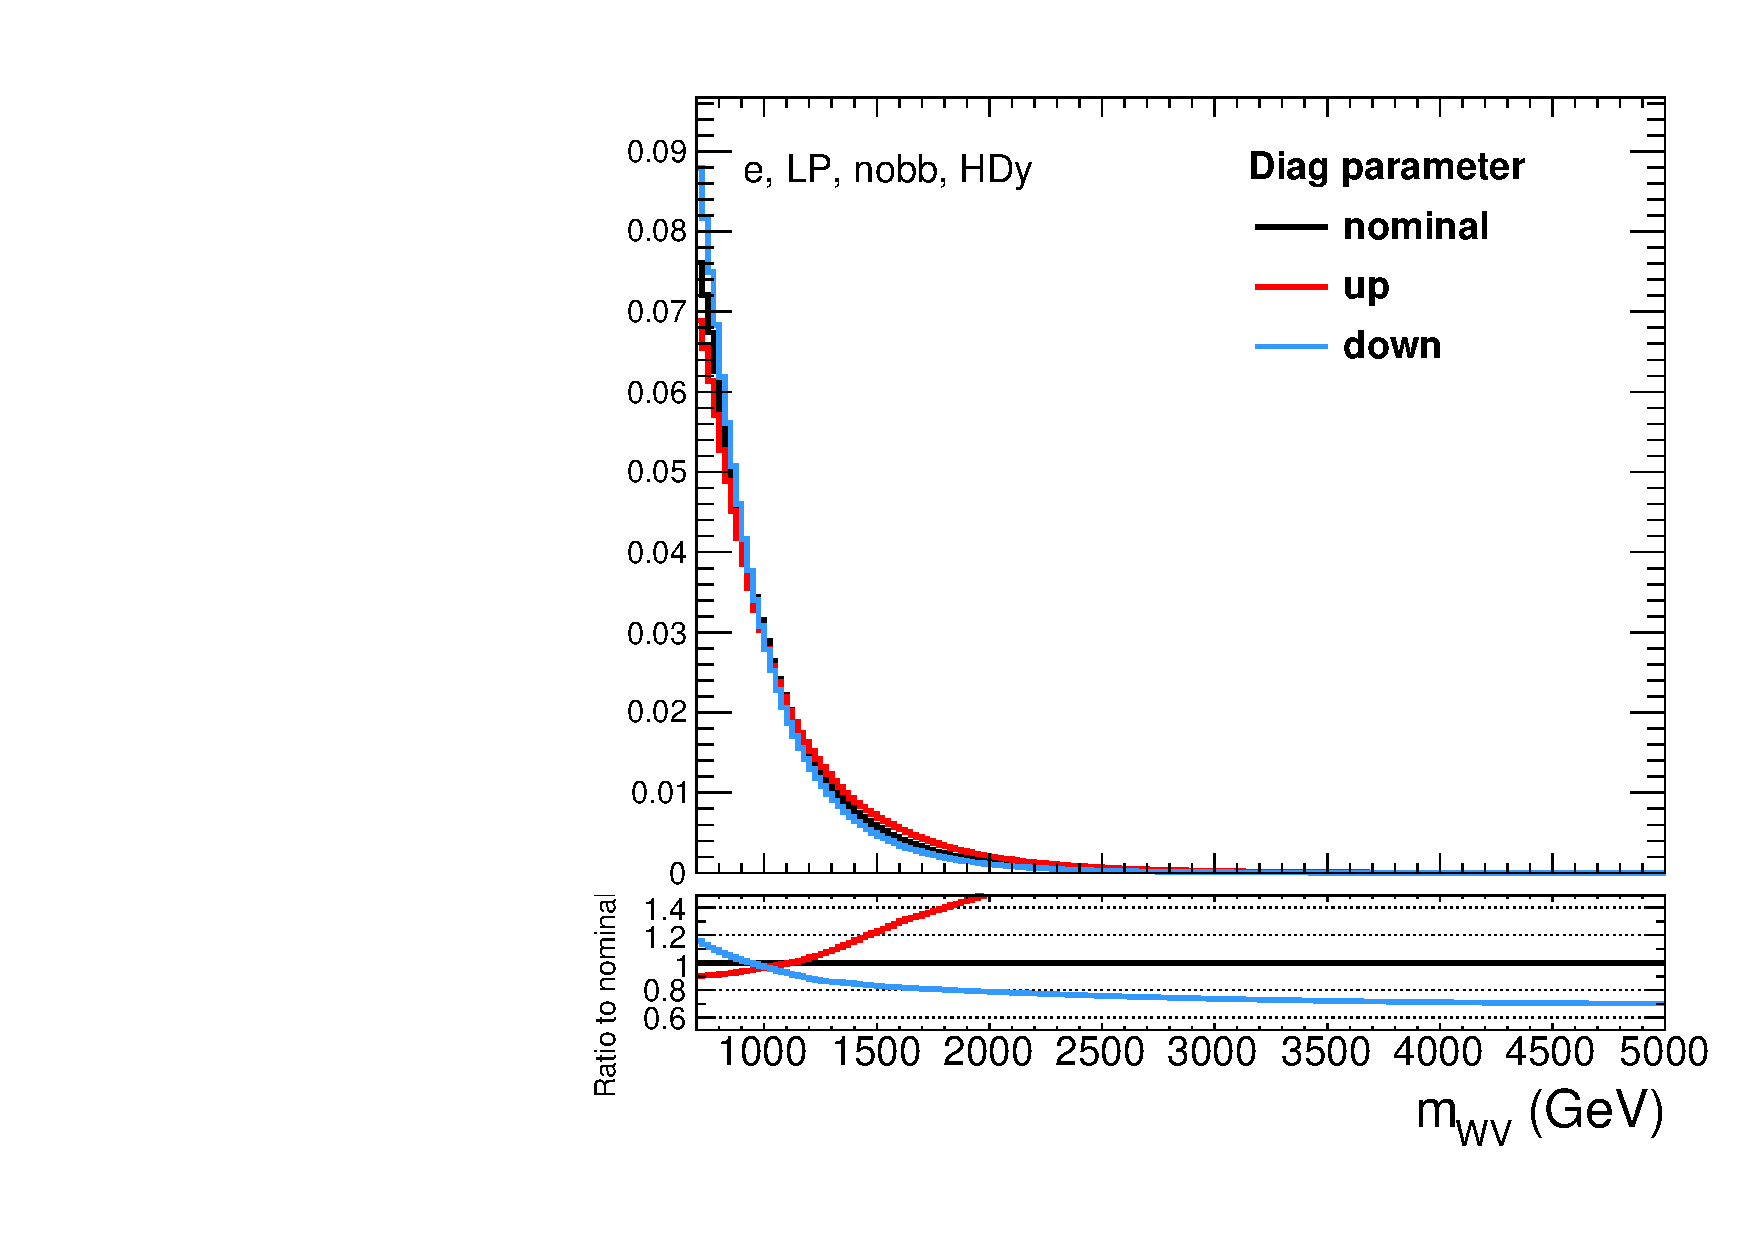
\includegraphics[width=0.21\textwidth]{fig/uncertainties/systs_nonRes_e_LP_nobb_HDy_Diag_ProjX.pdf}\\
  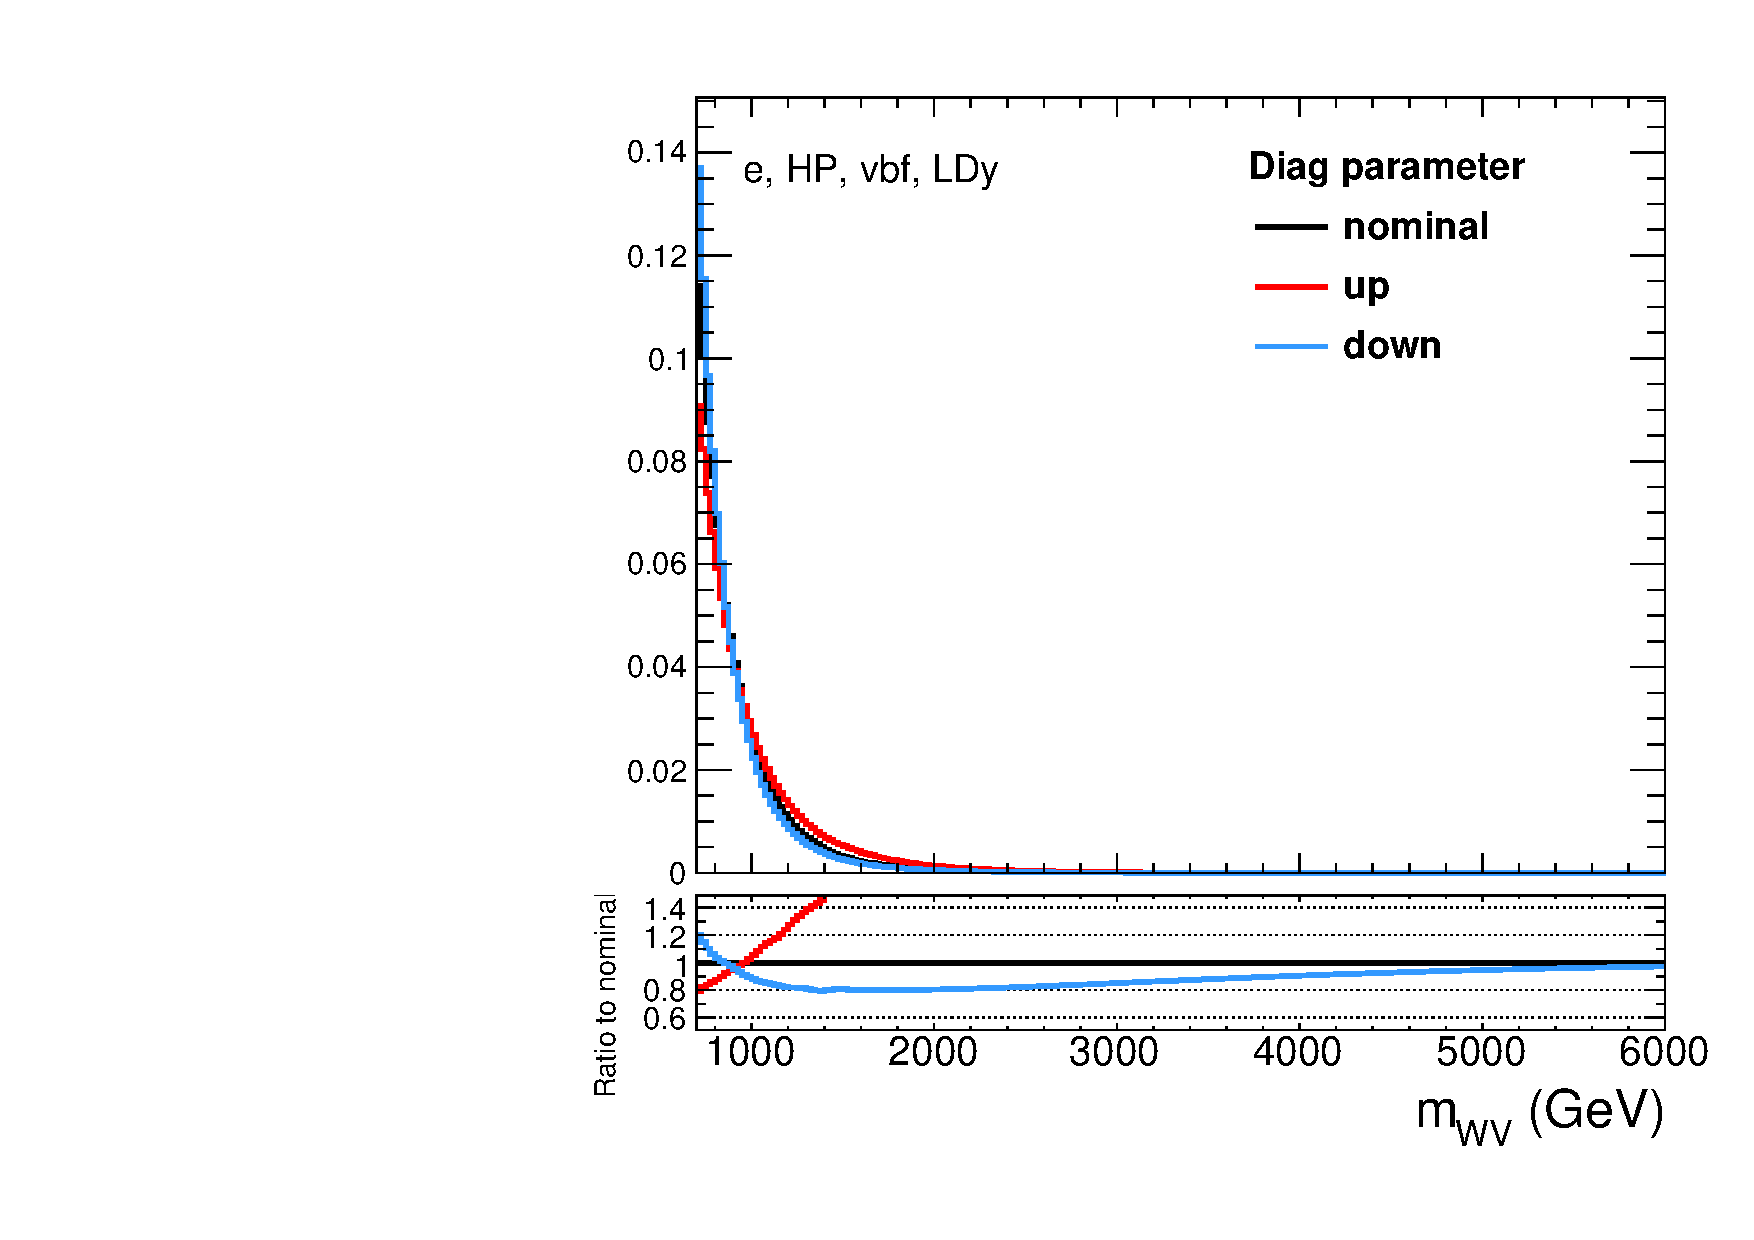
\includegraphics[width=0.21\textwidth]{fig/uncertainties/systs_nonRes_e_HP_vbf_LDy_Diag_ProjX.pdf}
  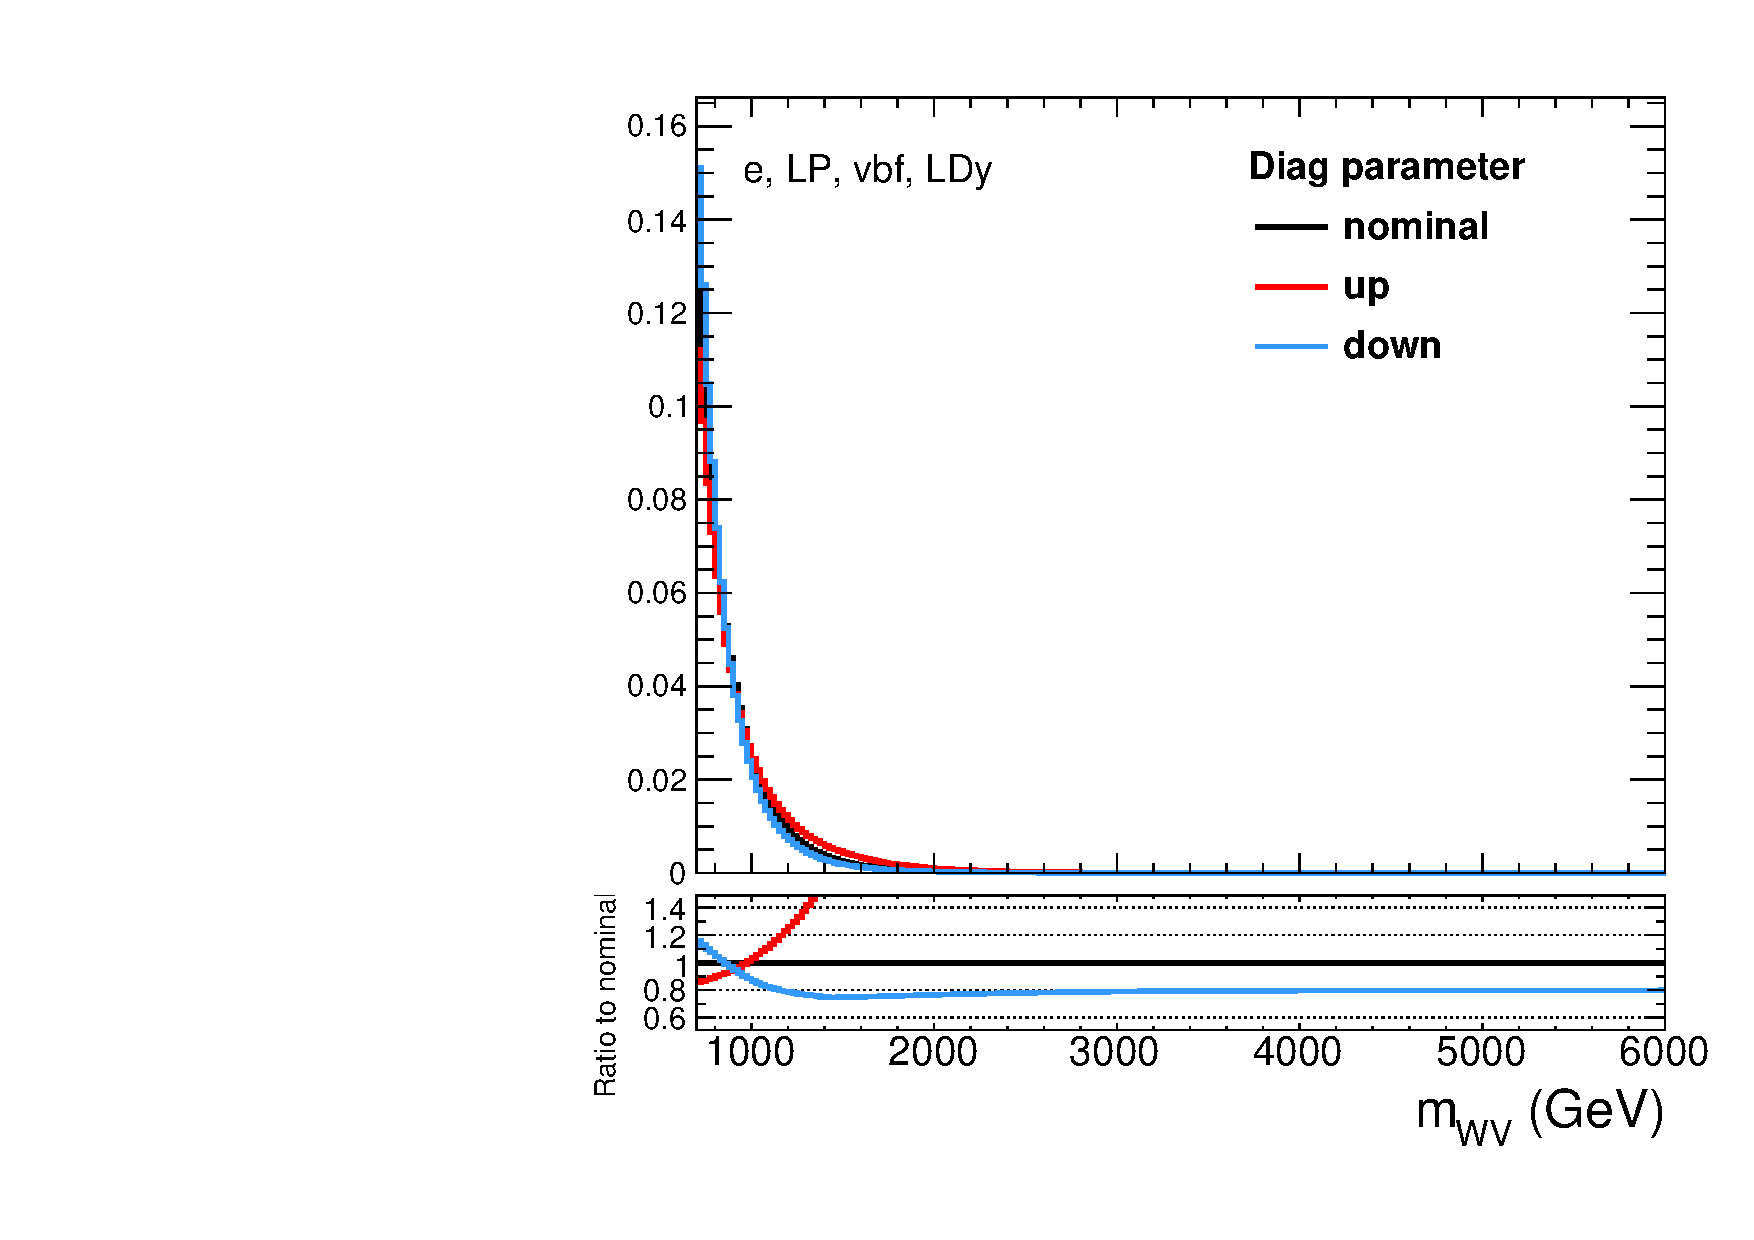
\includegraphics[width=0.21\textwidth]{fig/uncertainties/systs_nonRes_e_LP_vbf_LDy_Diag_ProjX.pdf}
  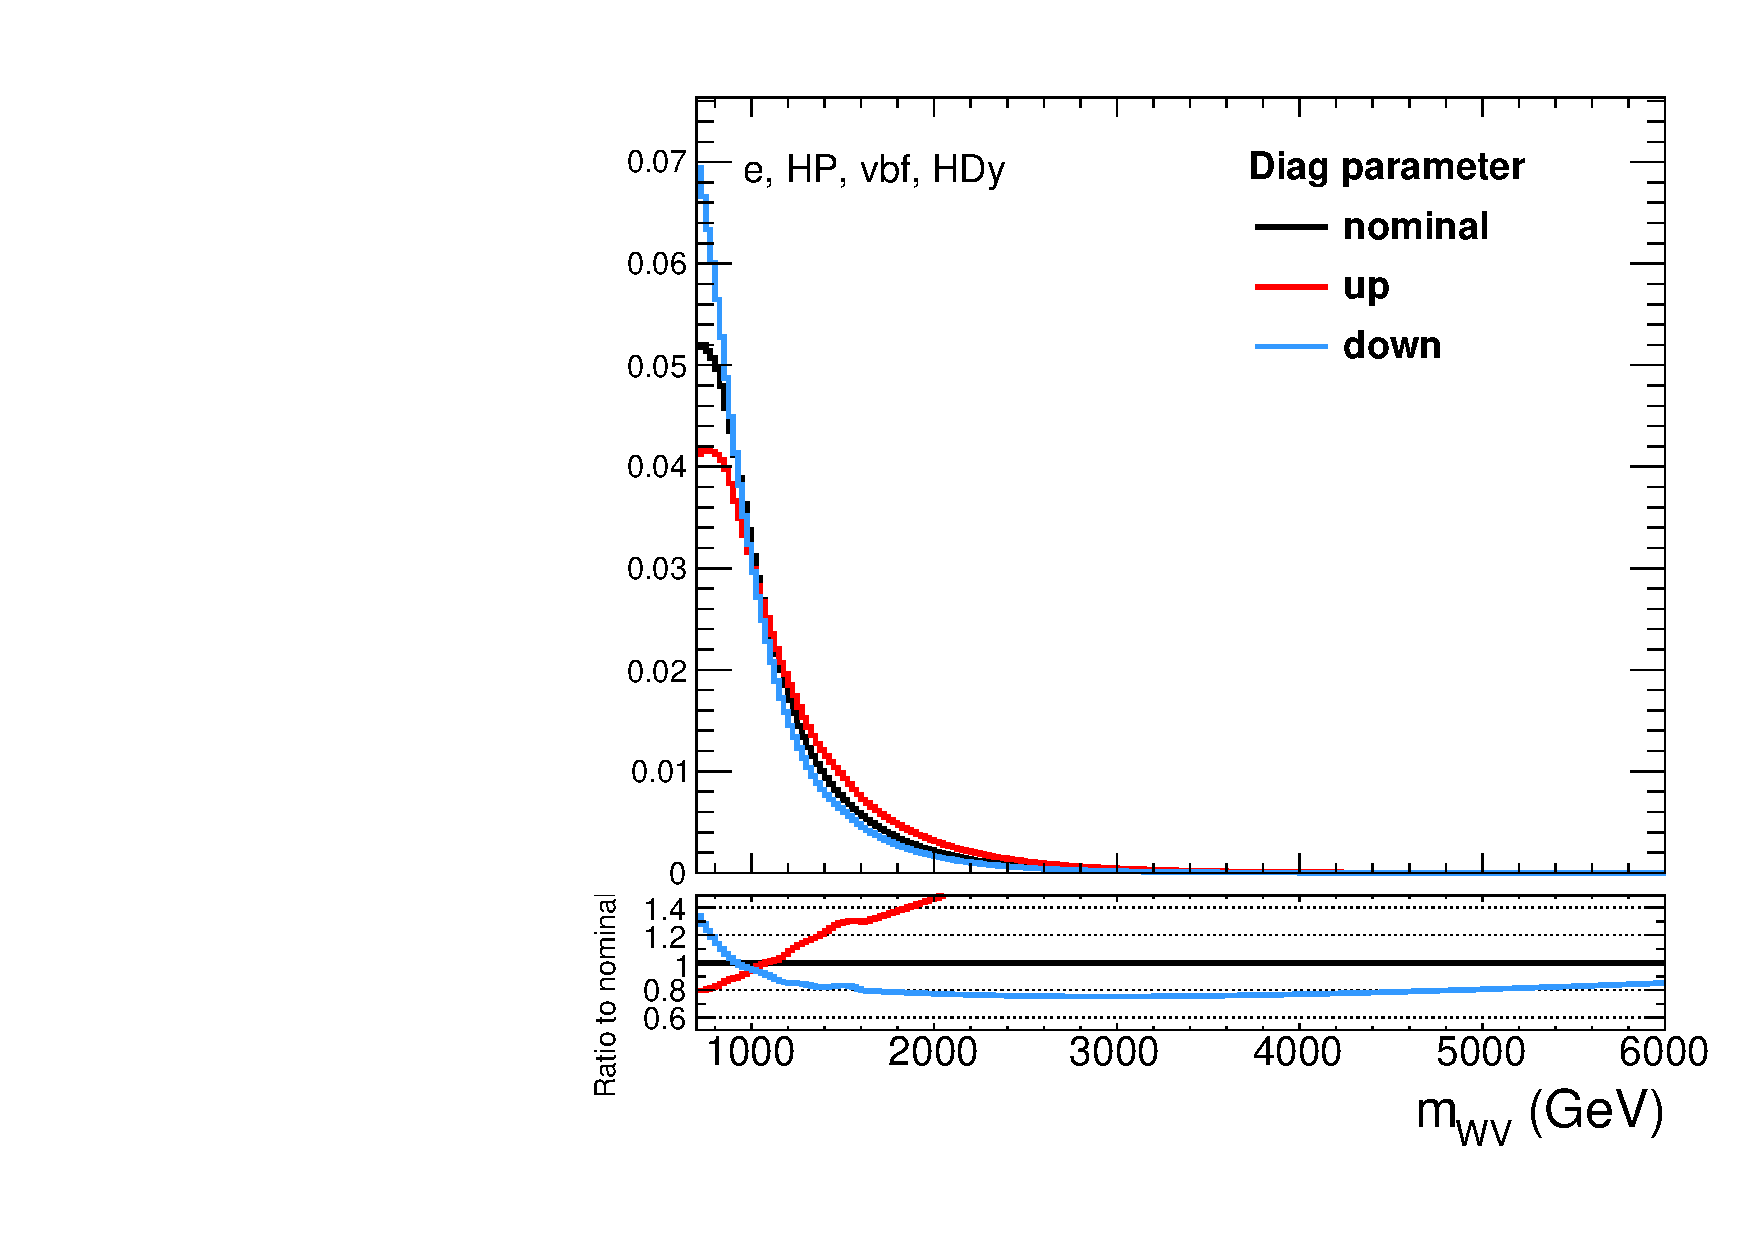
\includegraphics[width=0.21\textwidth]{fig/uncertainties/systs_nonRes_e_HP_vbf_HDy_Diag_ProjX.pdf}
  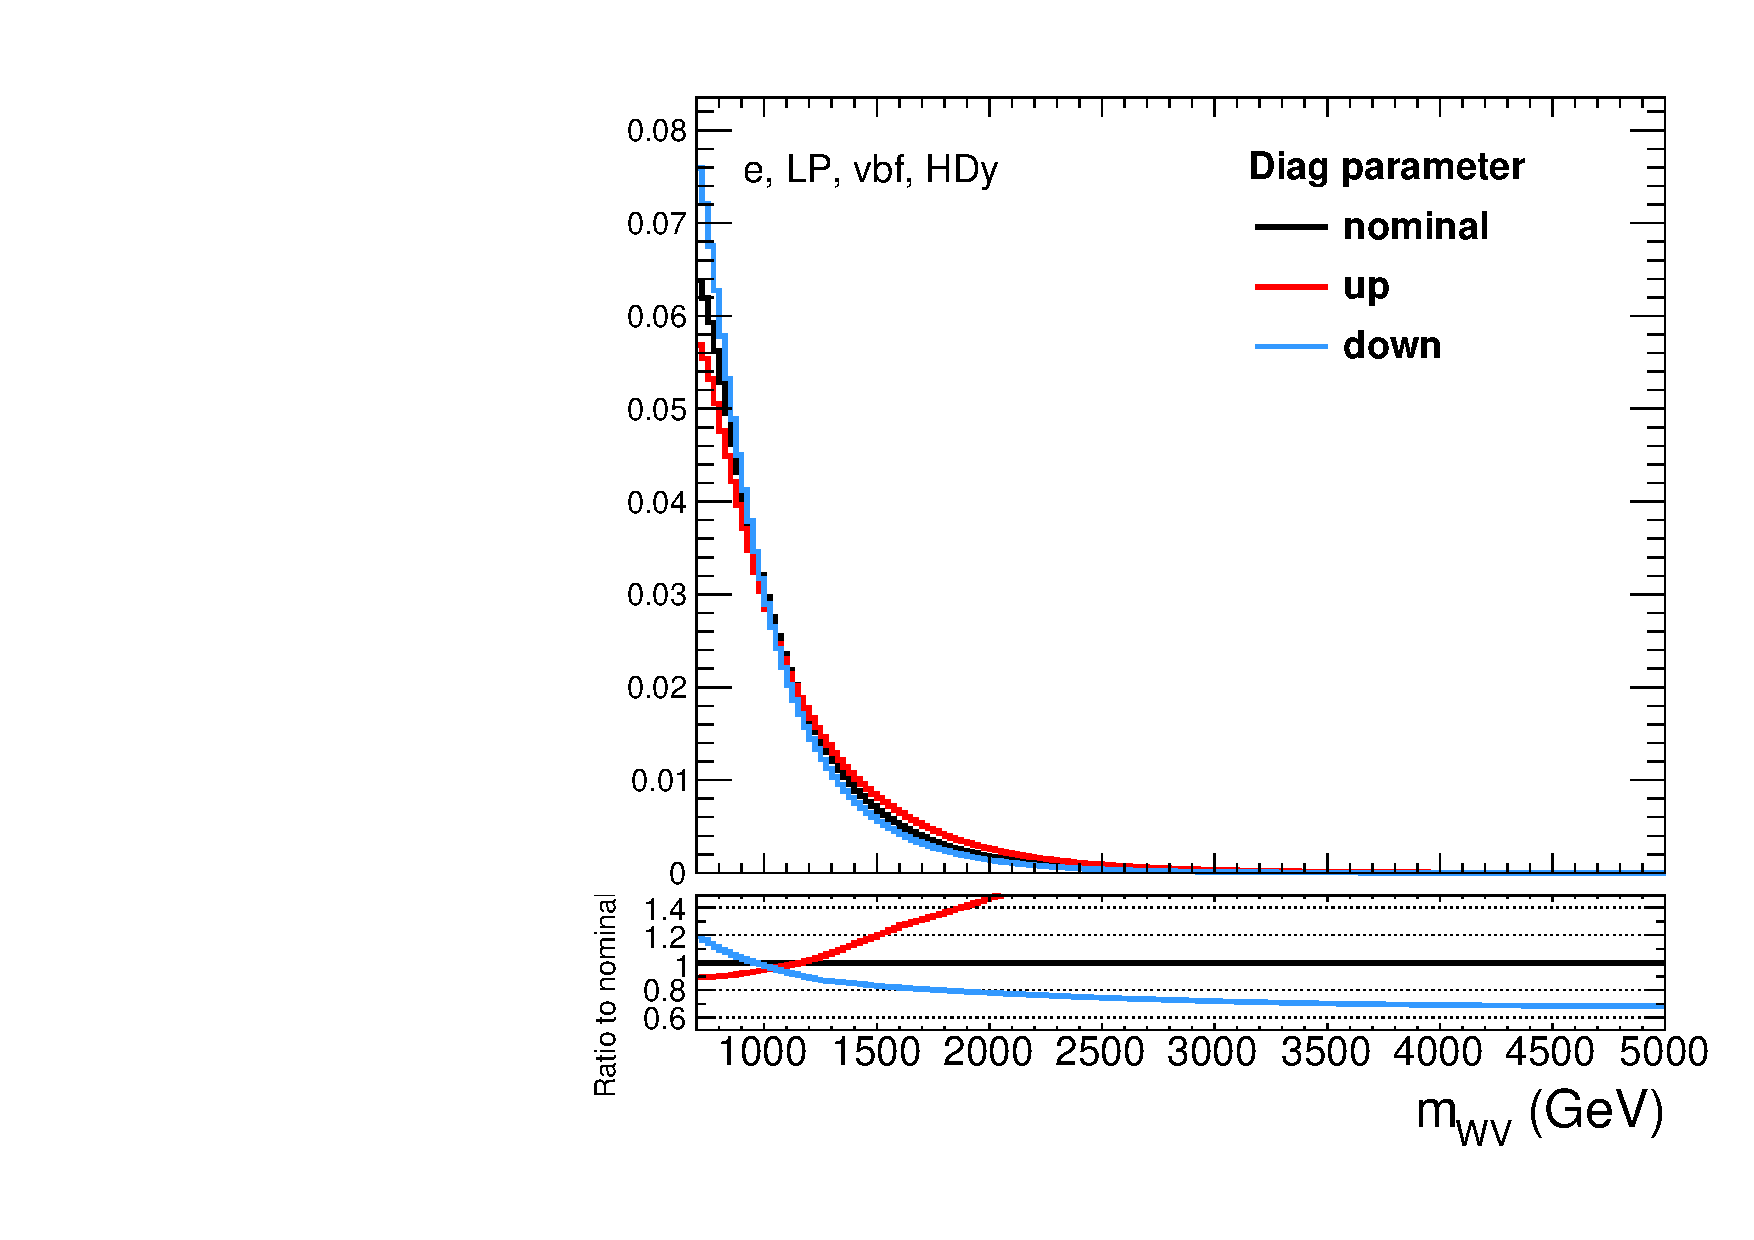
\includegraphics[width=0.21\textwidth]{fig/uncertainties/systs_nonRes_e_LP_vbf_HDy_Diag_ProjX.pdf}\\
  \caption{
    Projections of the nominal and alternative shapes of the non-resonant background onto the \MVV dimension obtained from applying $\pm3\sigma$ variations of the diagonal uncertainties for the electron channel.
    Columns 1 to 4: HP-LDy, LP-LDy, HP-HDy, LP-HDy.
    Rows 1 to 3: bb, nobb, vbf.
  }
  \label{fig:systNonResMVV_Diag}
\end{figure}

% Non-resonant jet shape variation
For the \MJ, we define two shape variations as well in order to account for hadronization-related effects:
\begin{itemize}
  \item {\bfseries LogWeight:} A reweighting of events based on the difference in the hadronization behavior in data versus MC using the hadronization-sensitive variable $\ln(\MJ^2/\pt)$.
  The weight is obtained by fitting the ratio of the data to MC in the $\ln(\MJ^2/\pt)$ distribution seen in figure~\ref{fig:logWeight} in the region dominated by \Wjets.
  This region is fitted with a function consisting of a Gaussian plus a constant term, with the reweighting of the events based on the fitted function.
  \item {\bfseries Soft drop mass scale:} Shift of the \MJ scale.
\end{itemize}
These nuisance parameters are also left uncorrelated across categories, with figures~\ref{fig:systNonResMJ_logWeight} and \ref{fig:systNonResMJ_MJJScale} showing the nominal and $\pm3\sigma$ alternative shapes projected onto the \MJ dimension for the logWeight and soft drop mass scale uncertainties.

\begin{figure}[htbp]
  \centering
  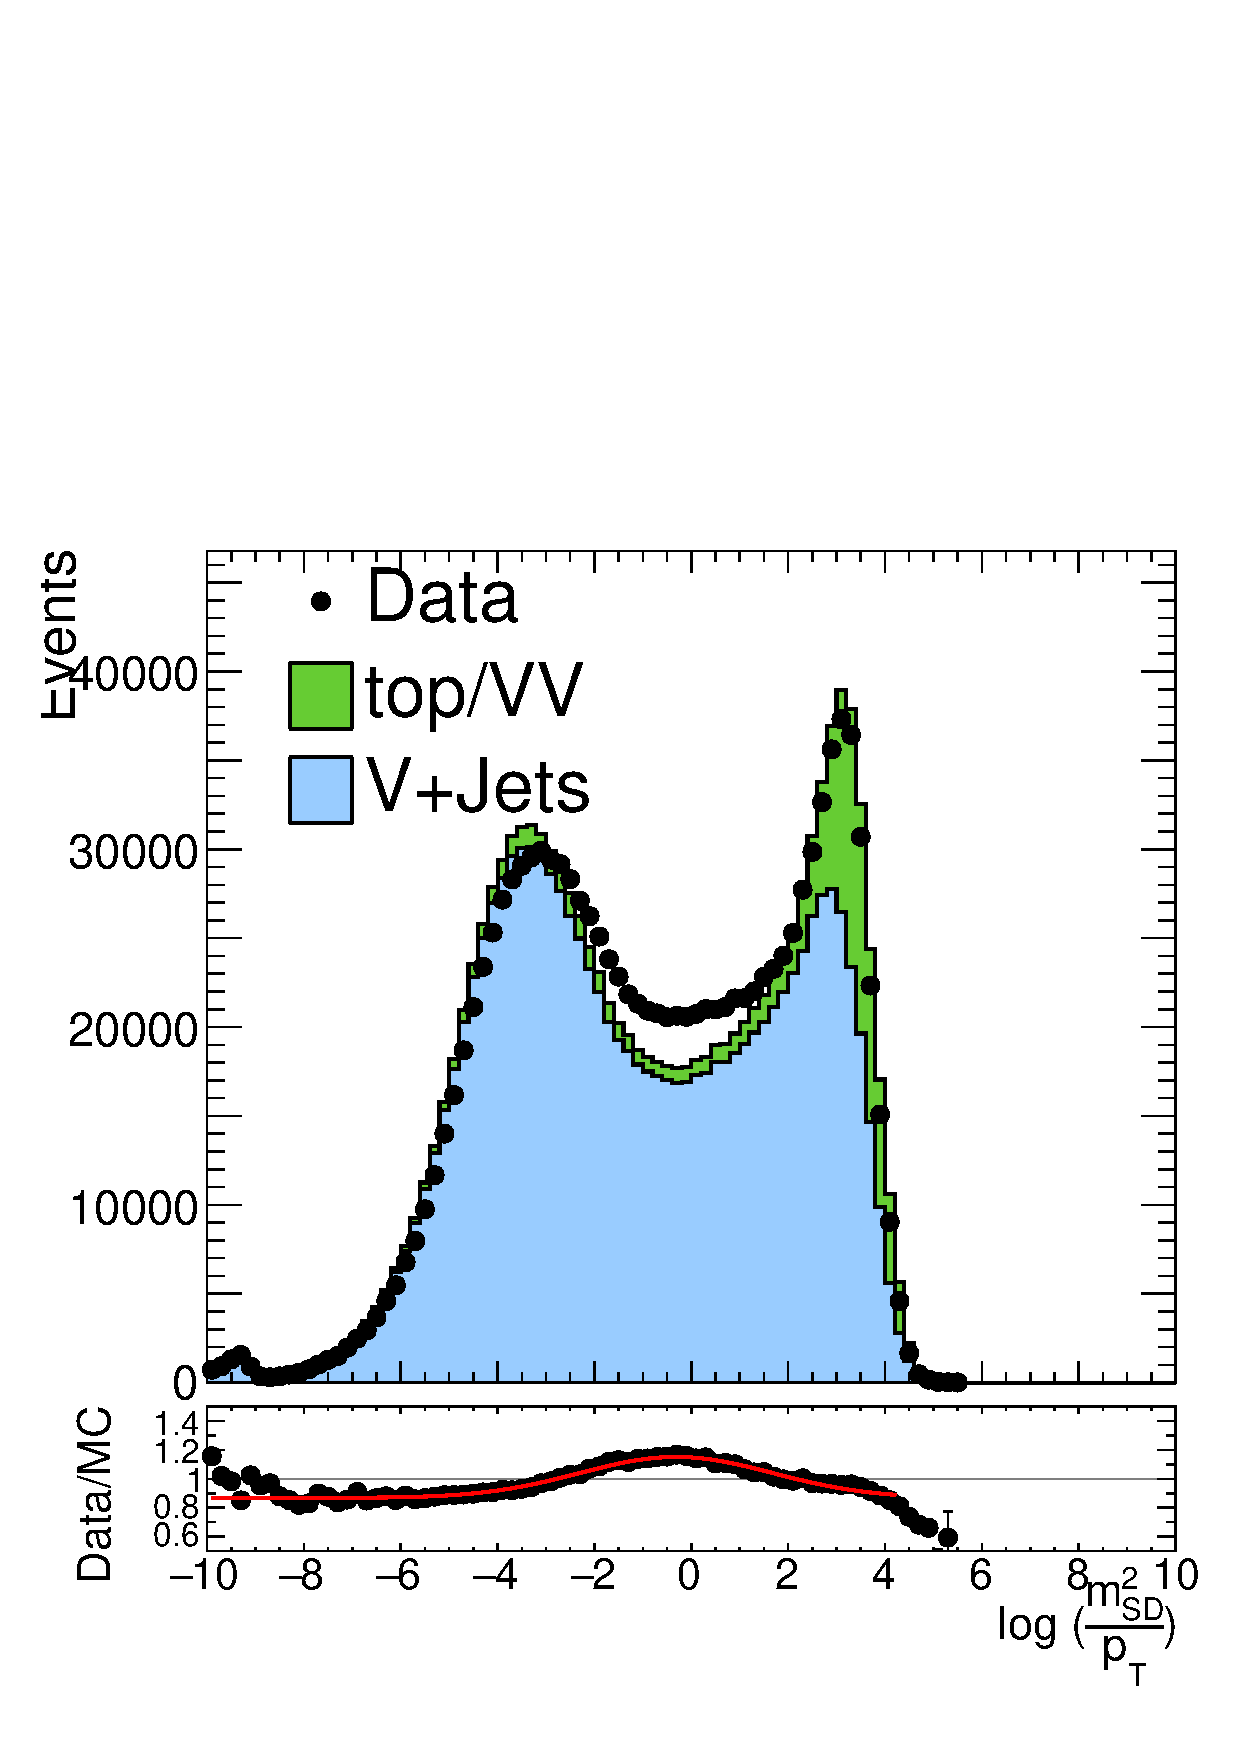
\includegraphics[width=0.4\textwidth]{fig/uncertainties/logWeight.pdf}
  \caption{
    Comparison between the Run 2 data and MC of the distributions for $\ln(\MJ^2/\pt)$ with all categories merged.
  }
  \label{fig:logWeight}
\end{figure}

\begin{figure}[htbp]
  \centering
  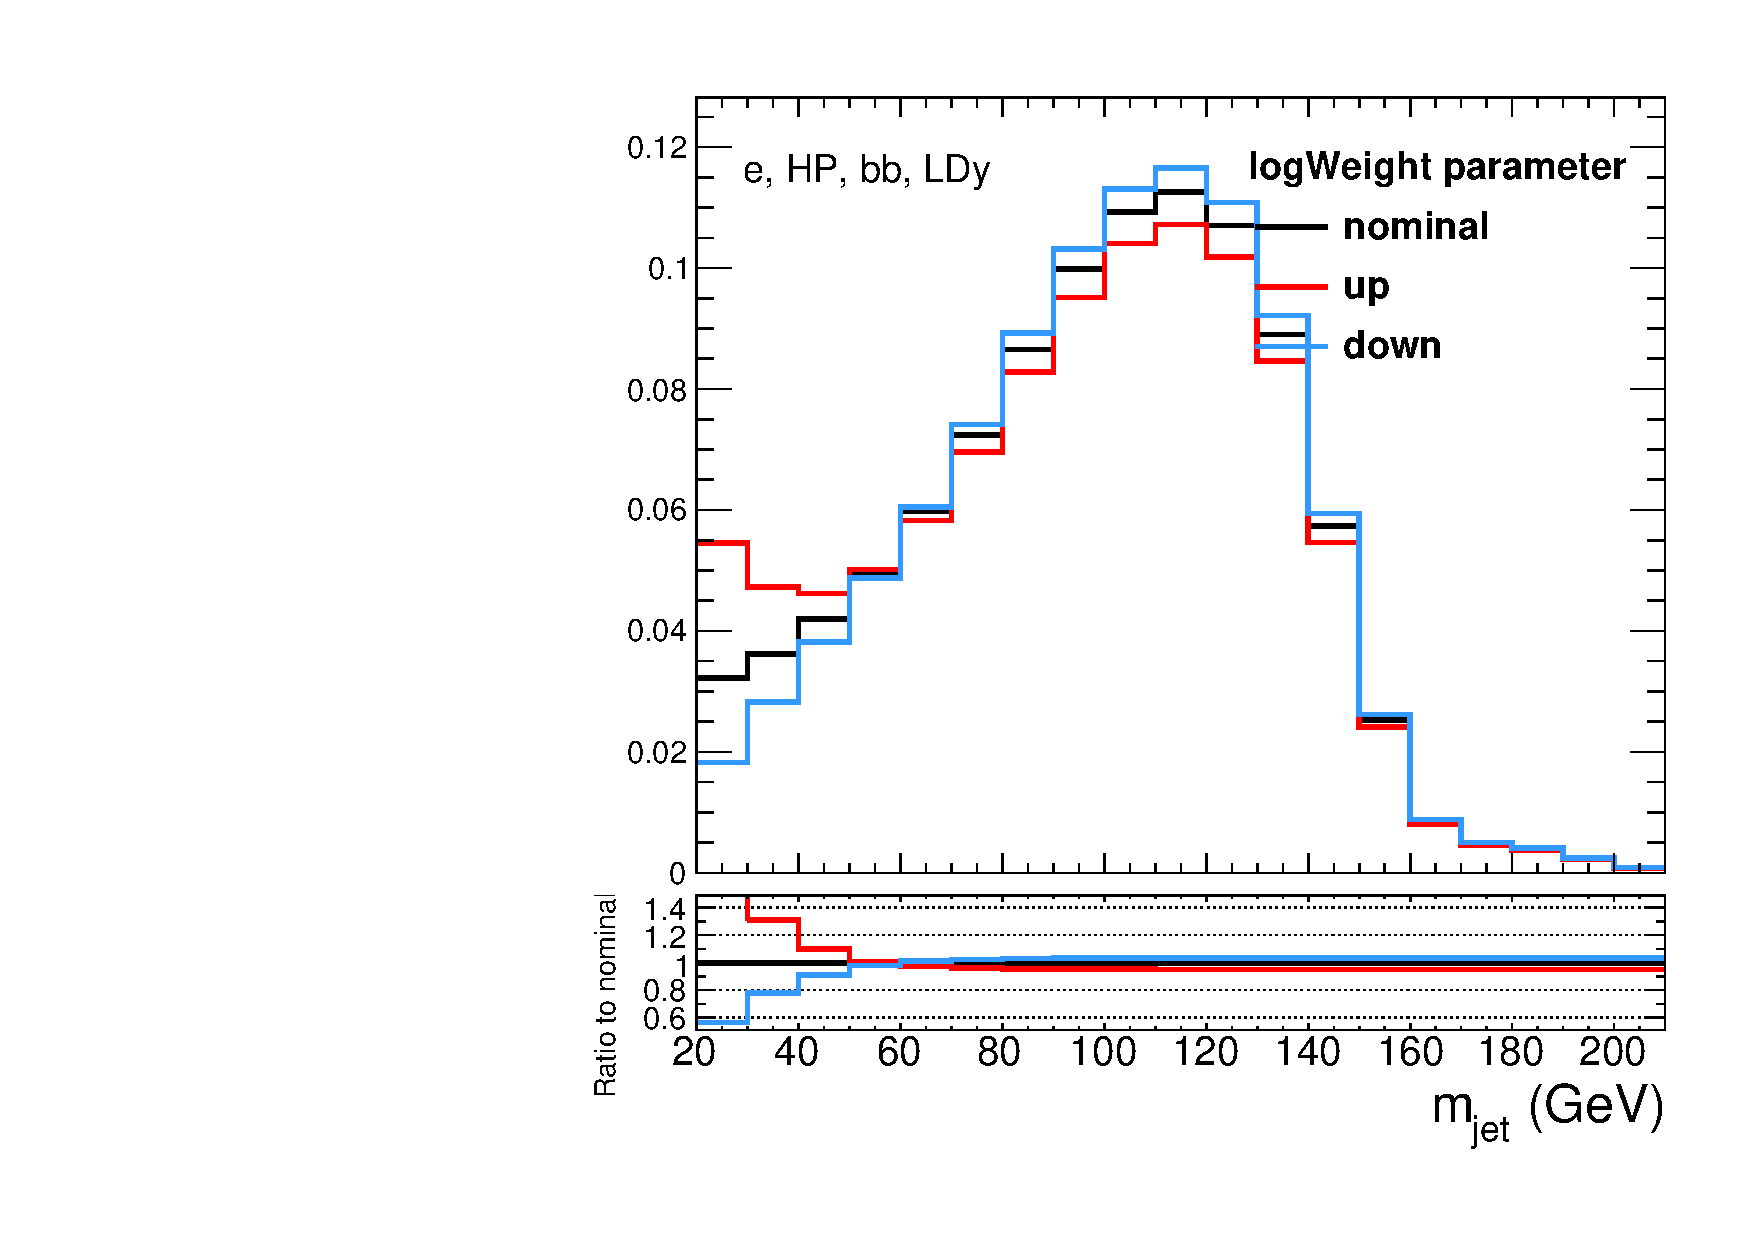
\includegraphics[width=0.21\textwidth]{fig/uncertainties/systs_nonRes_e_HP_bb_LDy_logWeight_ProjY.pdf}
  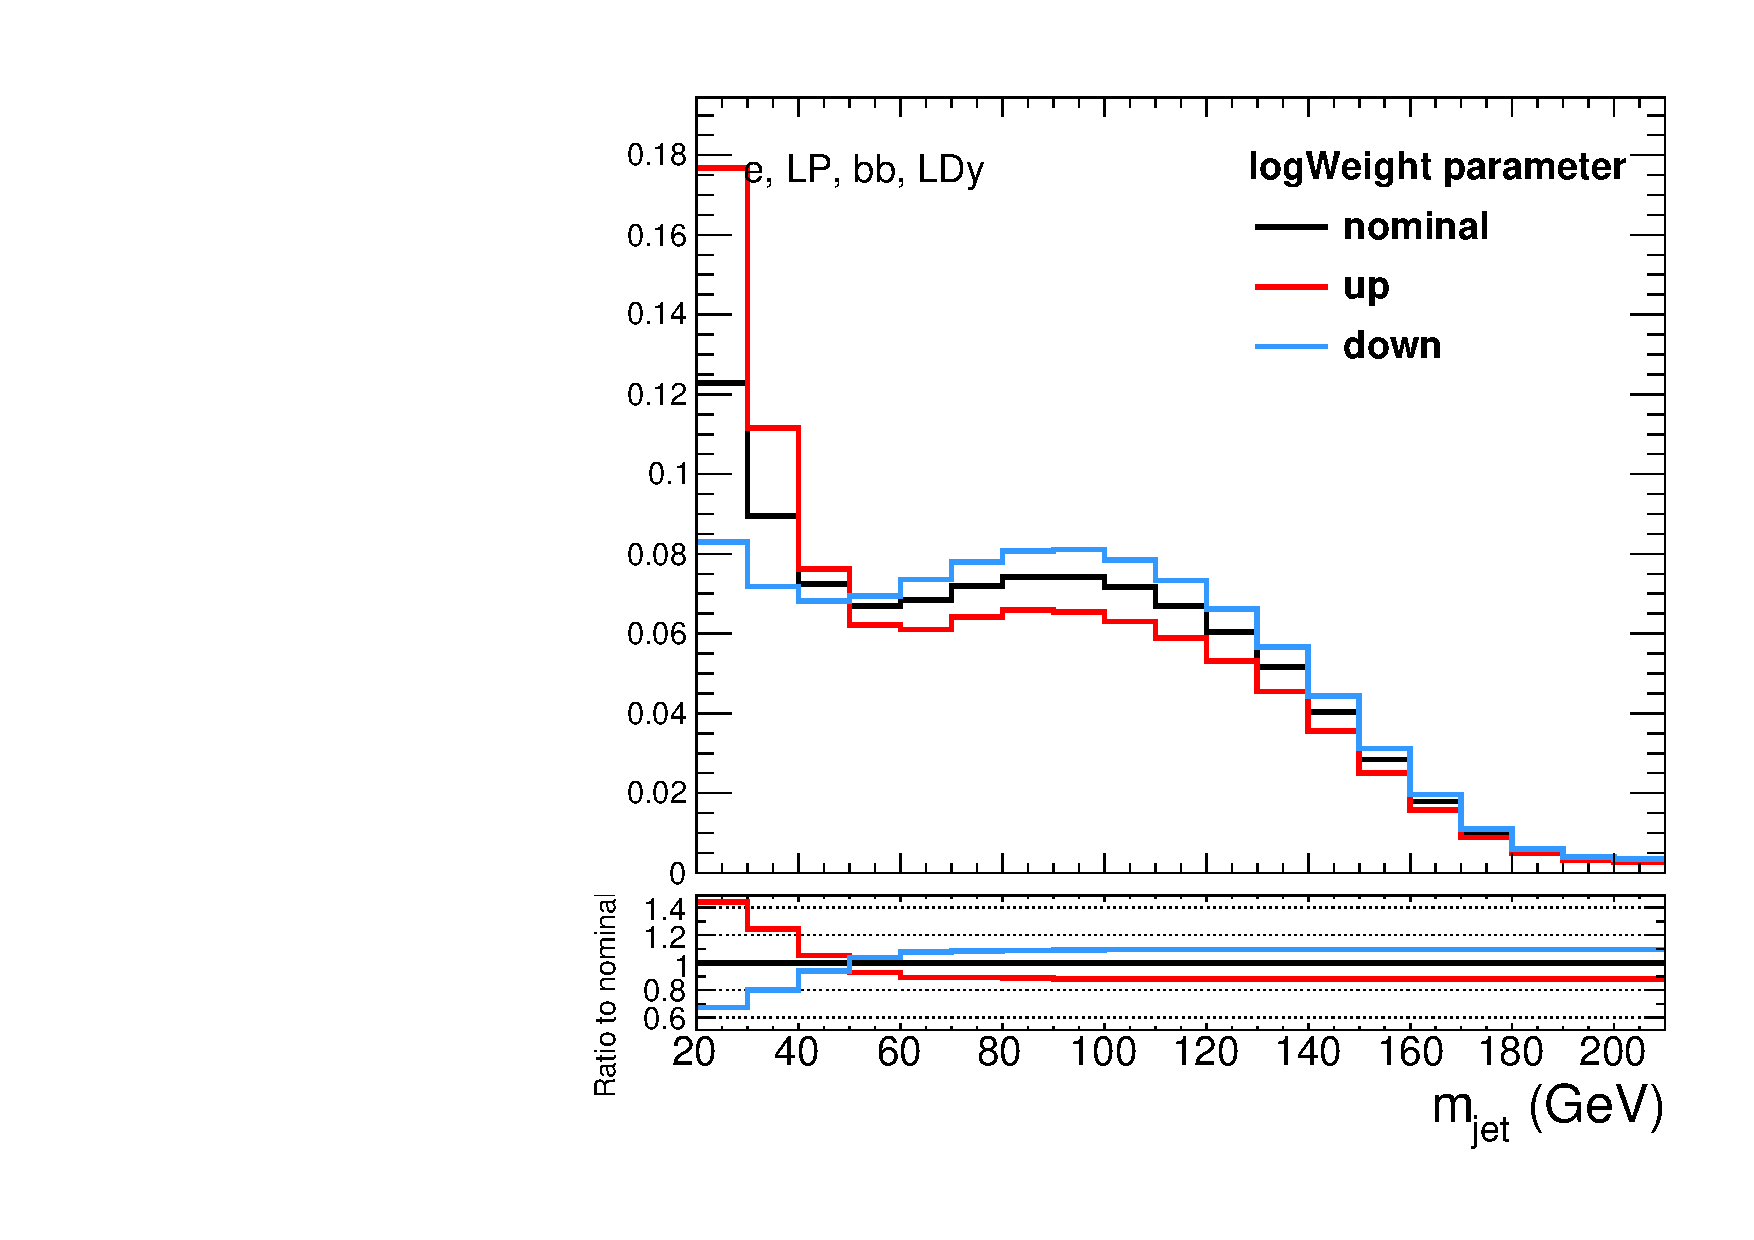
\includegraphics[width=0.21\textwidth]{fig/uncertainties/systs_nonRes_e_LP_bb_LDy_logWeight_ProjY.pdf}
  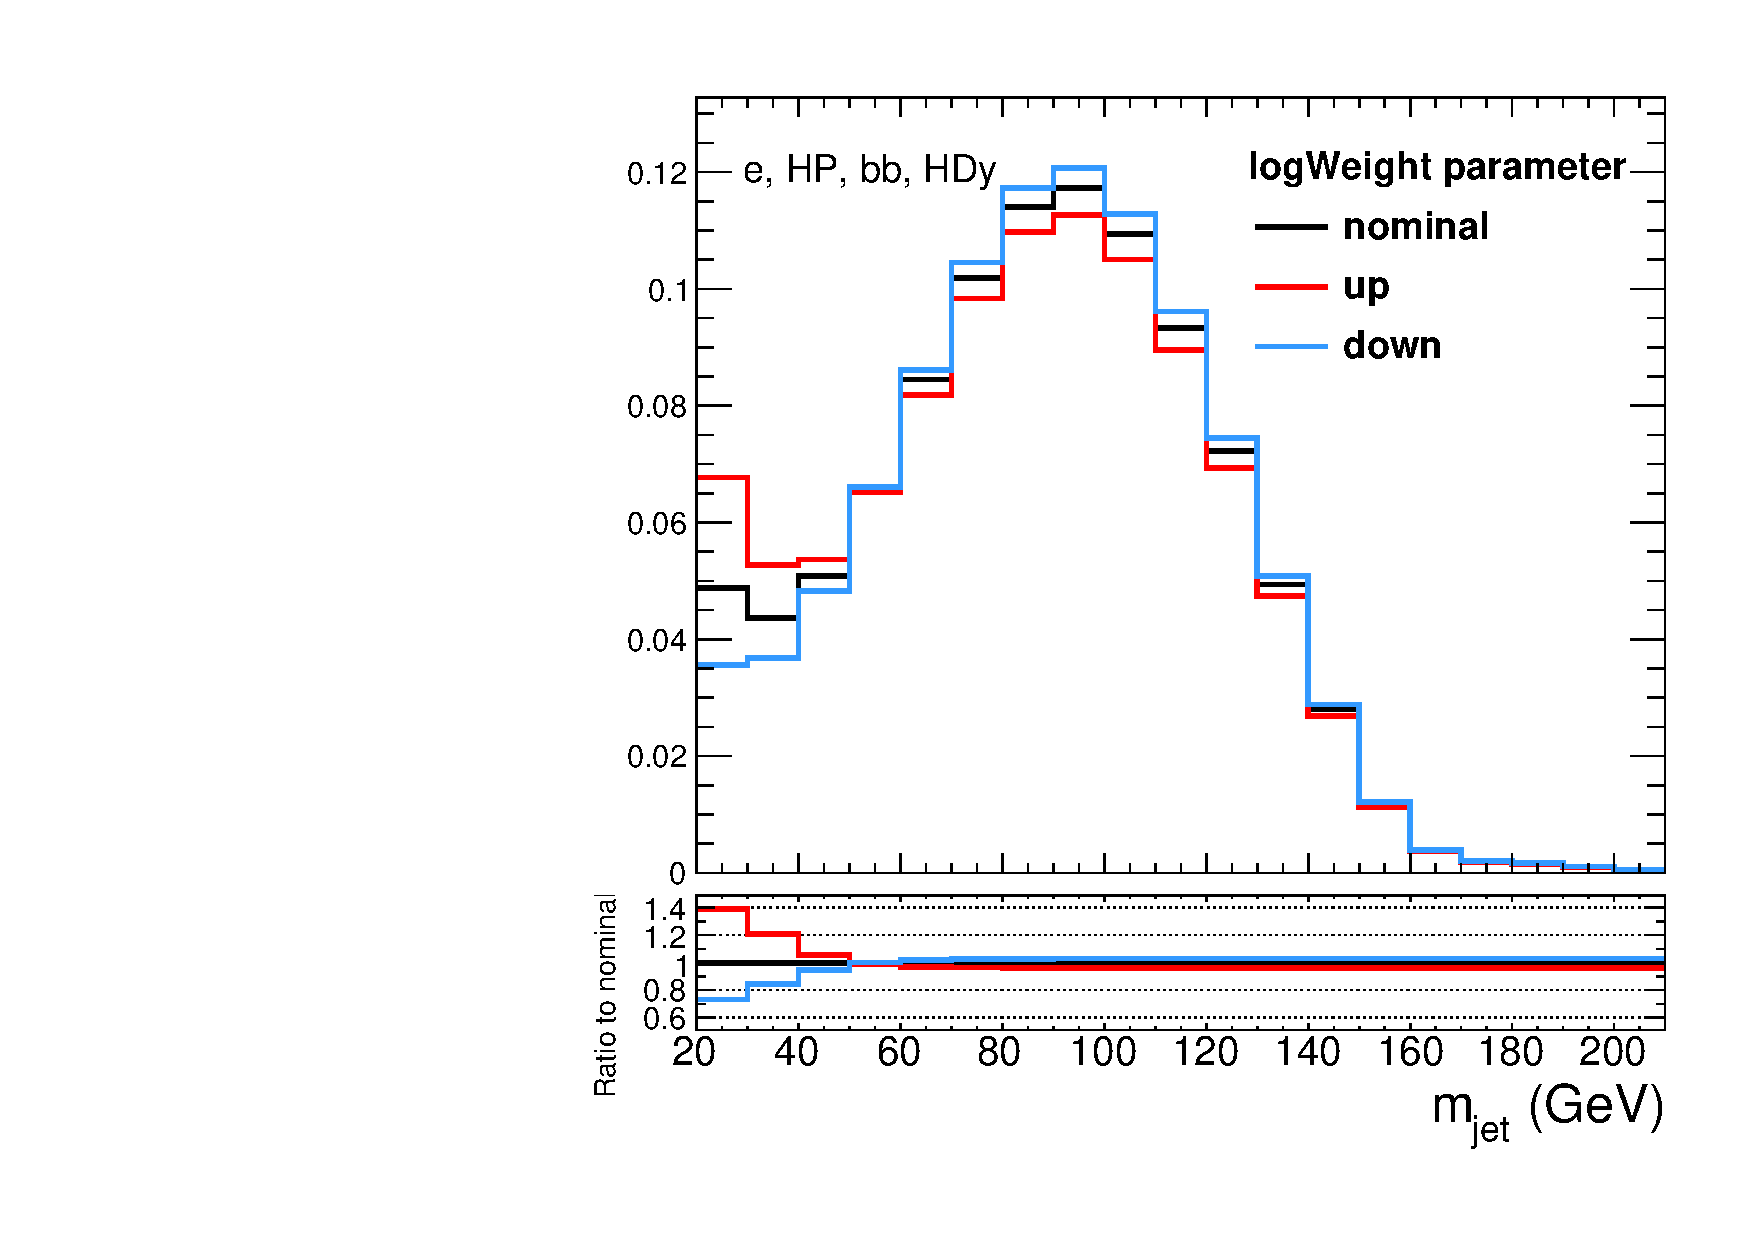
\includegraphics[width=0.21\textwidth]{fig/uncertainties/systs_nonRes_e_HP_bb_HDy_logWeight_ProjY.pdf}
  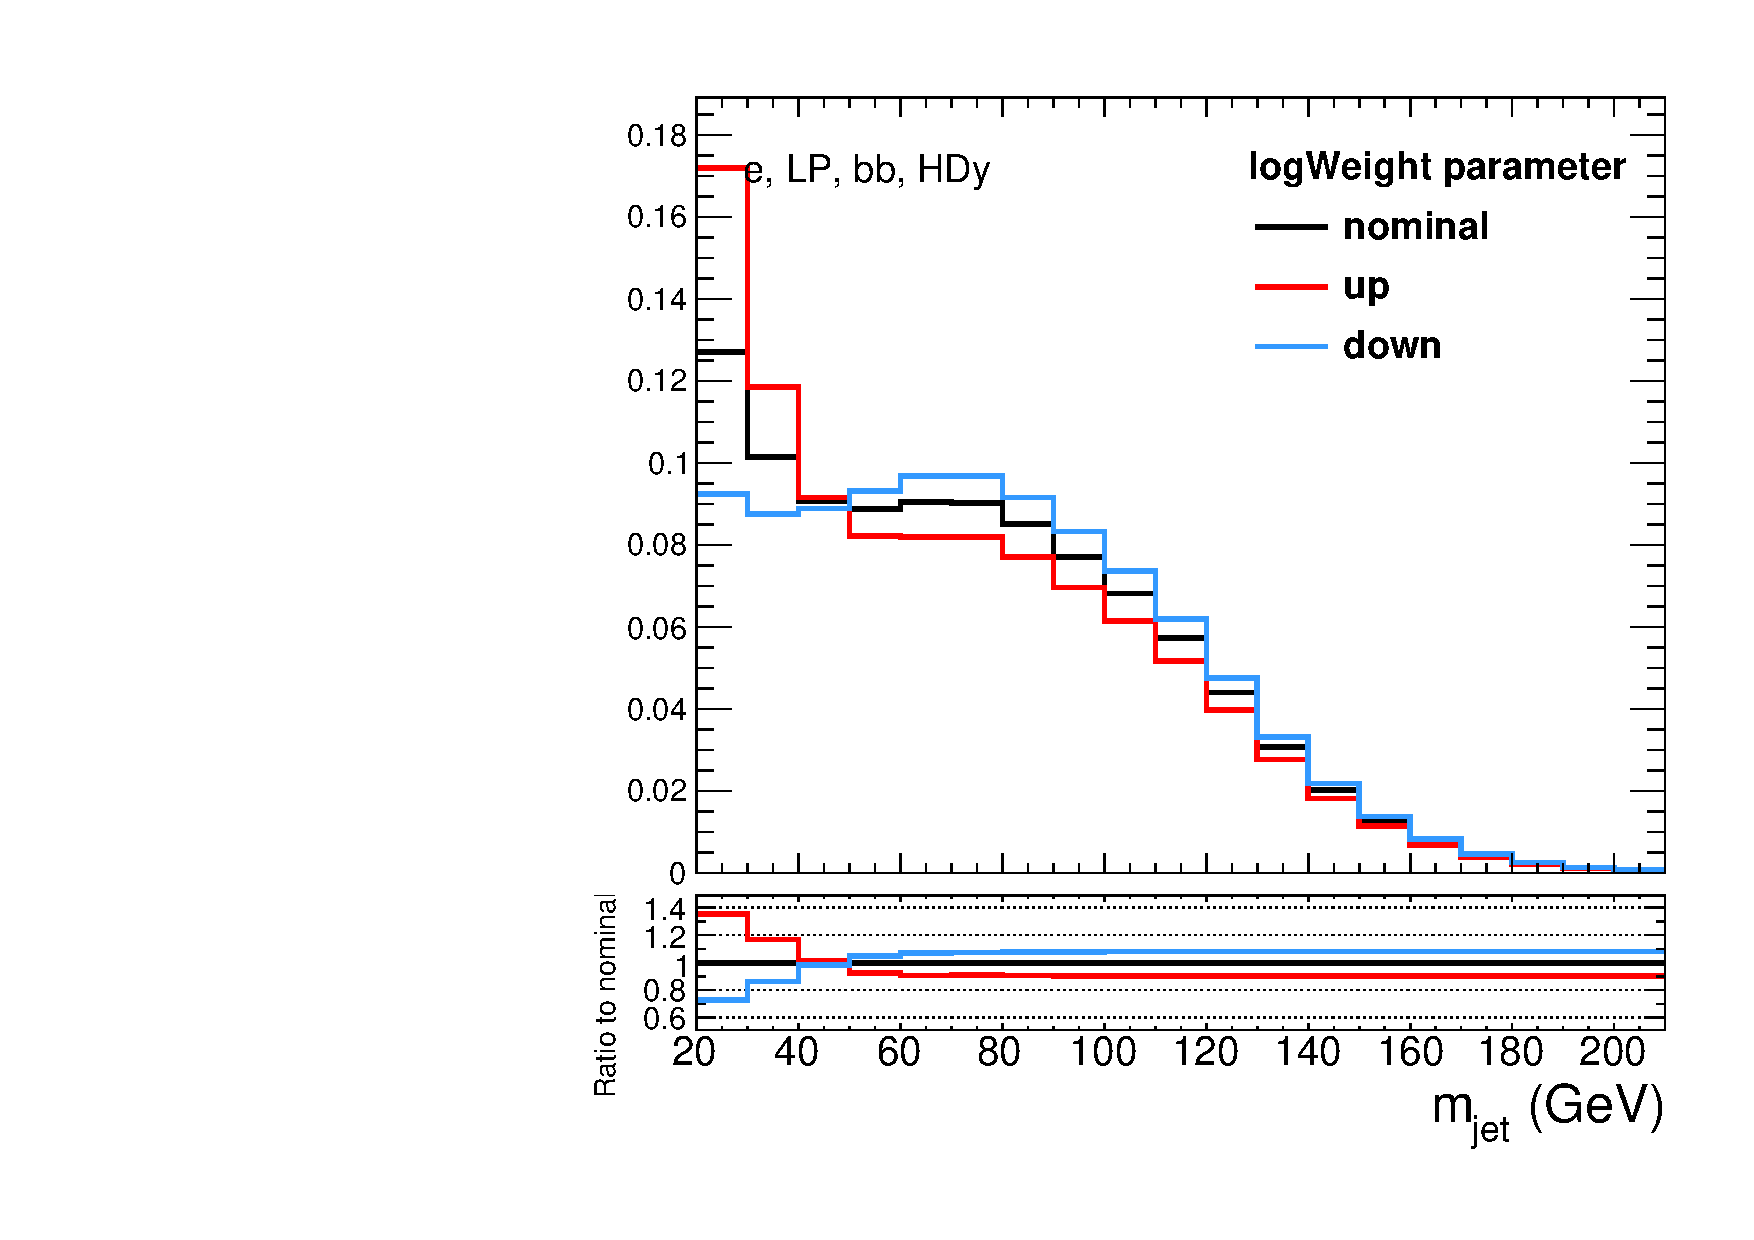
\includegraphics[width=0.21\textwidth]{fig/uncertainties/systs_nonRes_e_LP_bb_HDy_logWeight_ProjY.pdf}\\
  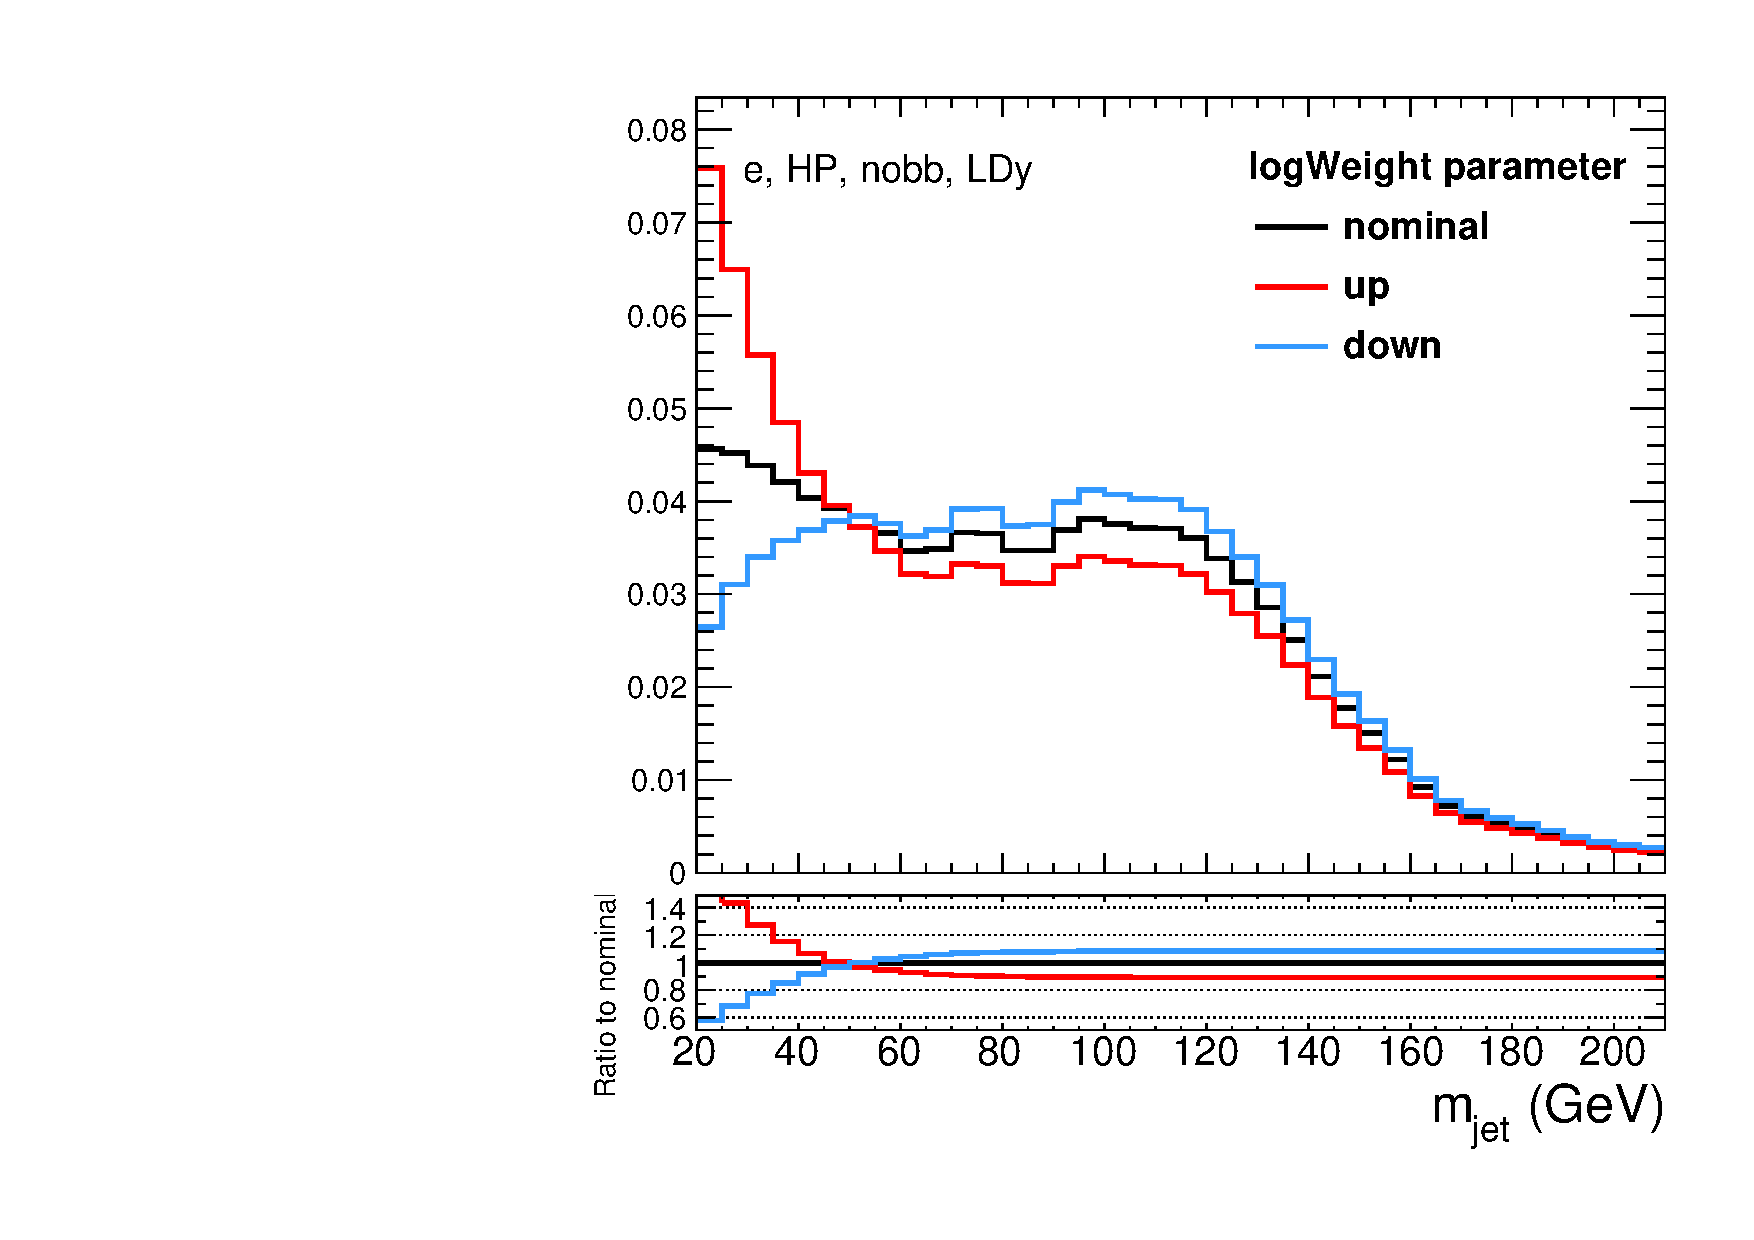
\includegraphics[width=0.21\textwidth]{fig/uncertainties/systs_nonRes_e_HP_nobb_LDy_logWeight_ProjY.pdf}
  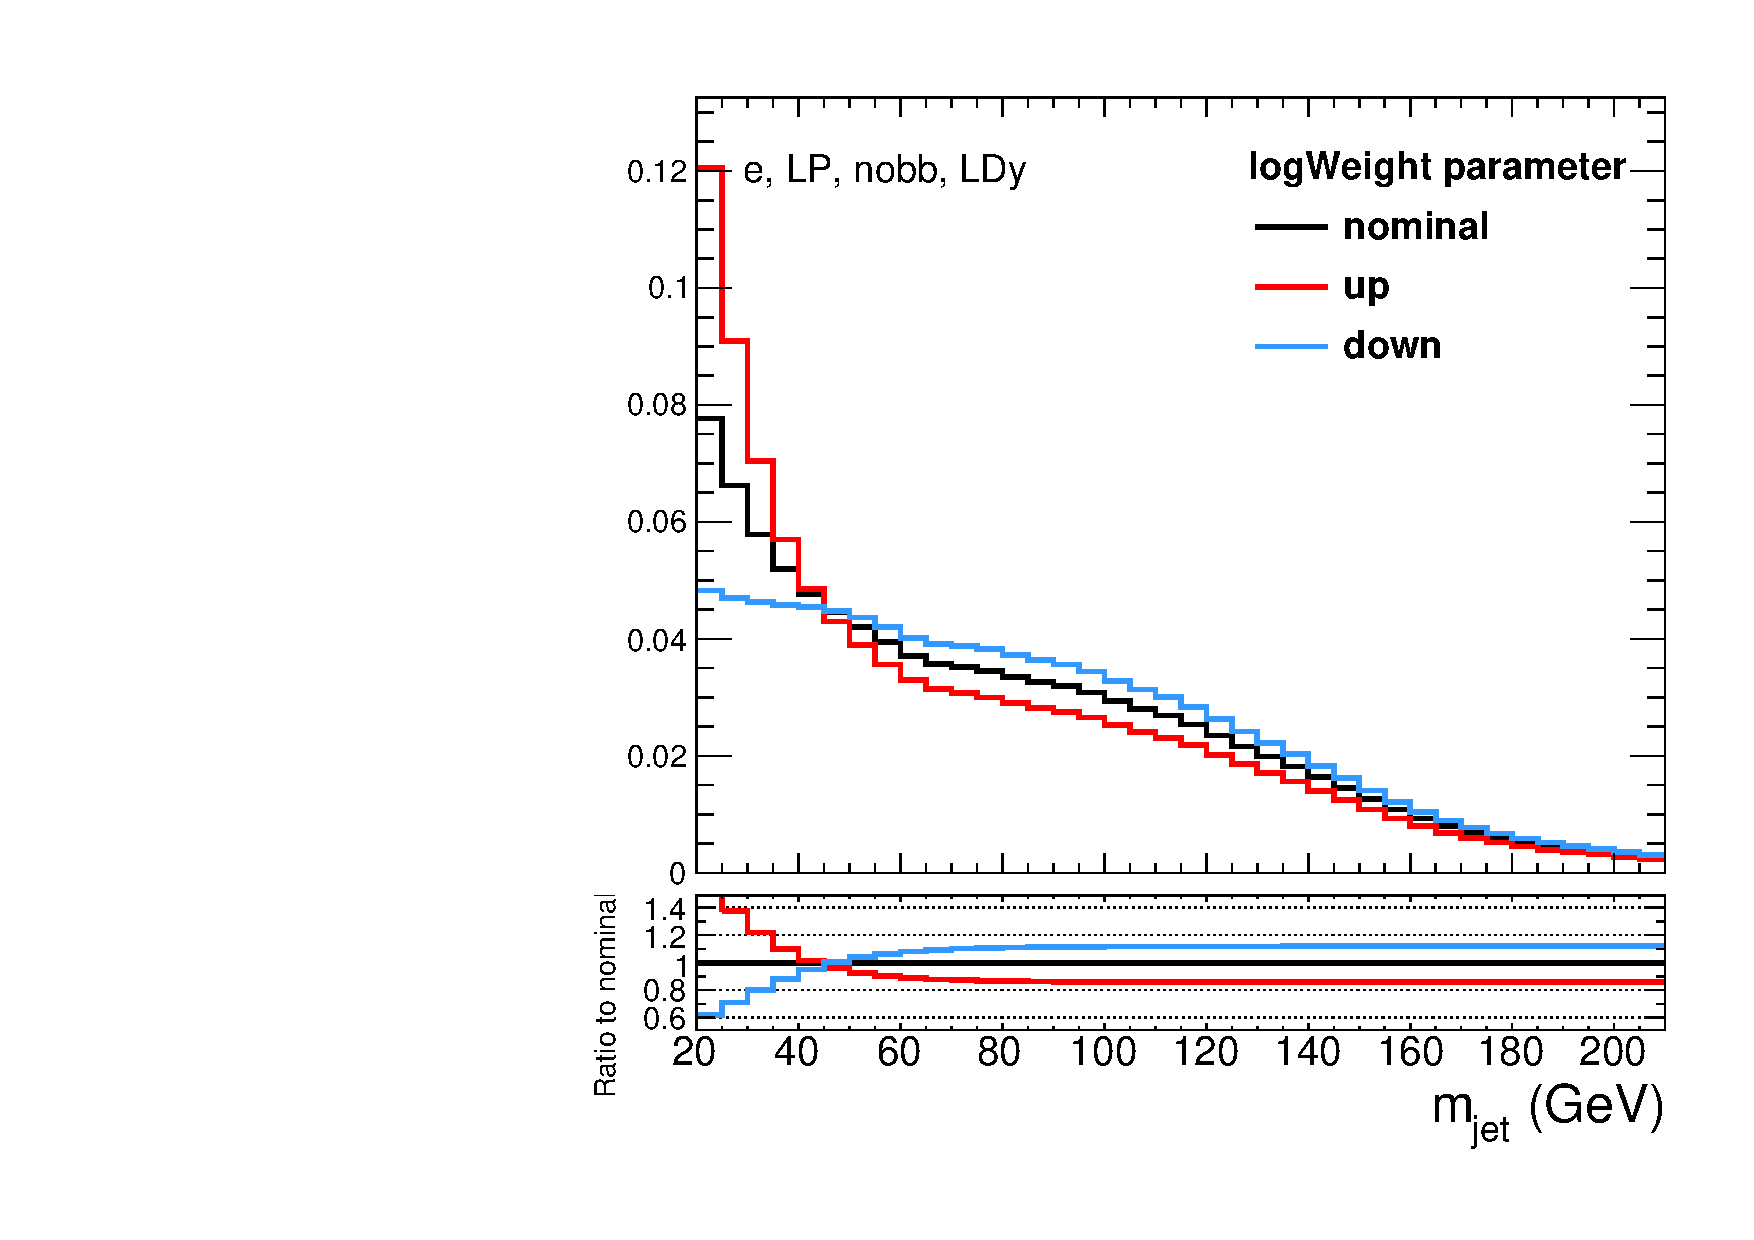
\includegraphics[width=0.21\textwidth]{fig/uncertainties/systs_nonRes_e_LP_nobb_LDy_logWeight_ProjY.pdf}
  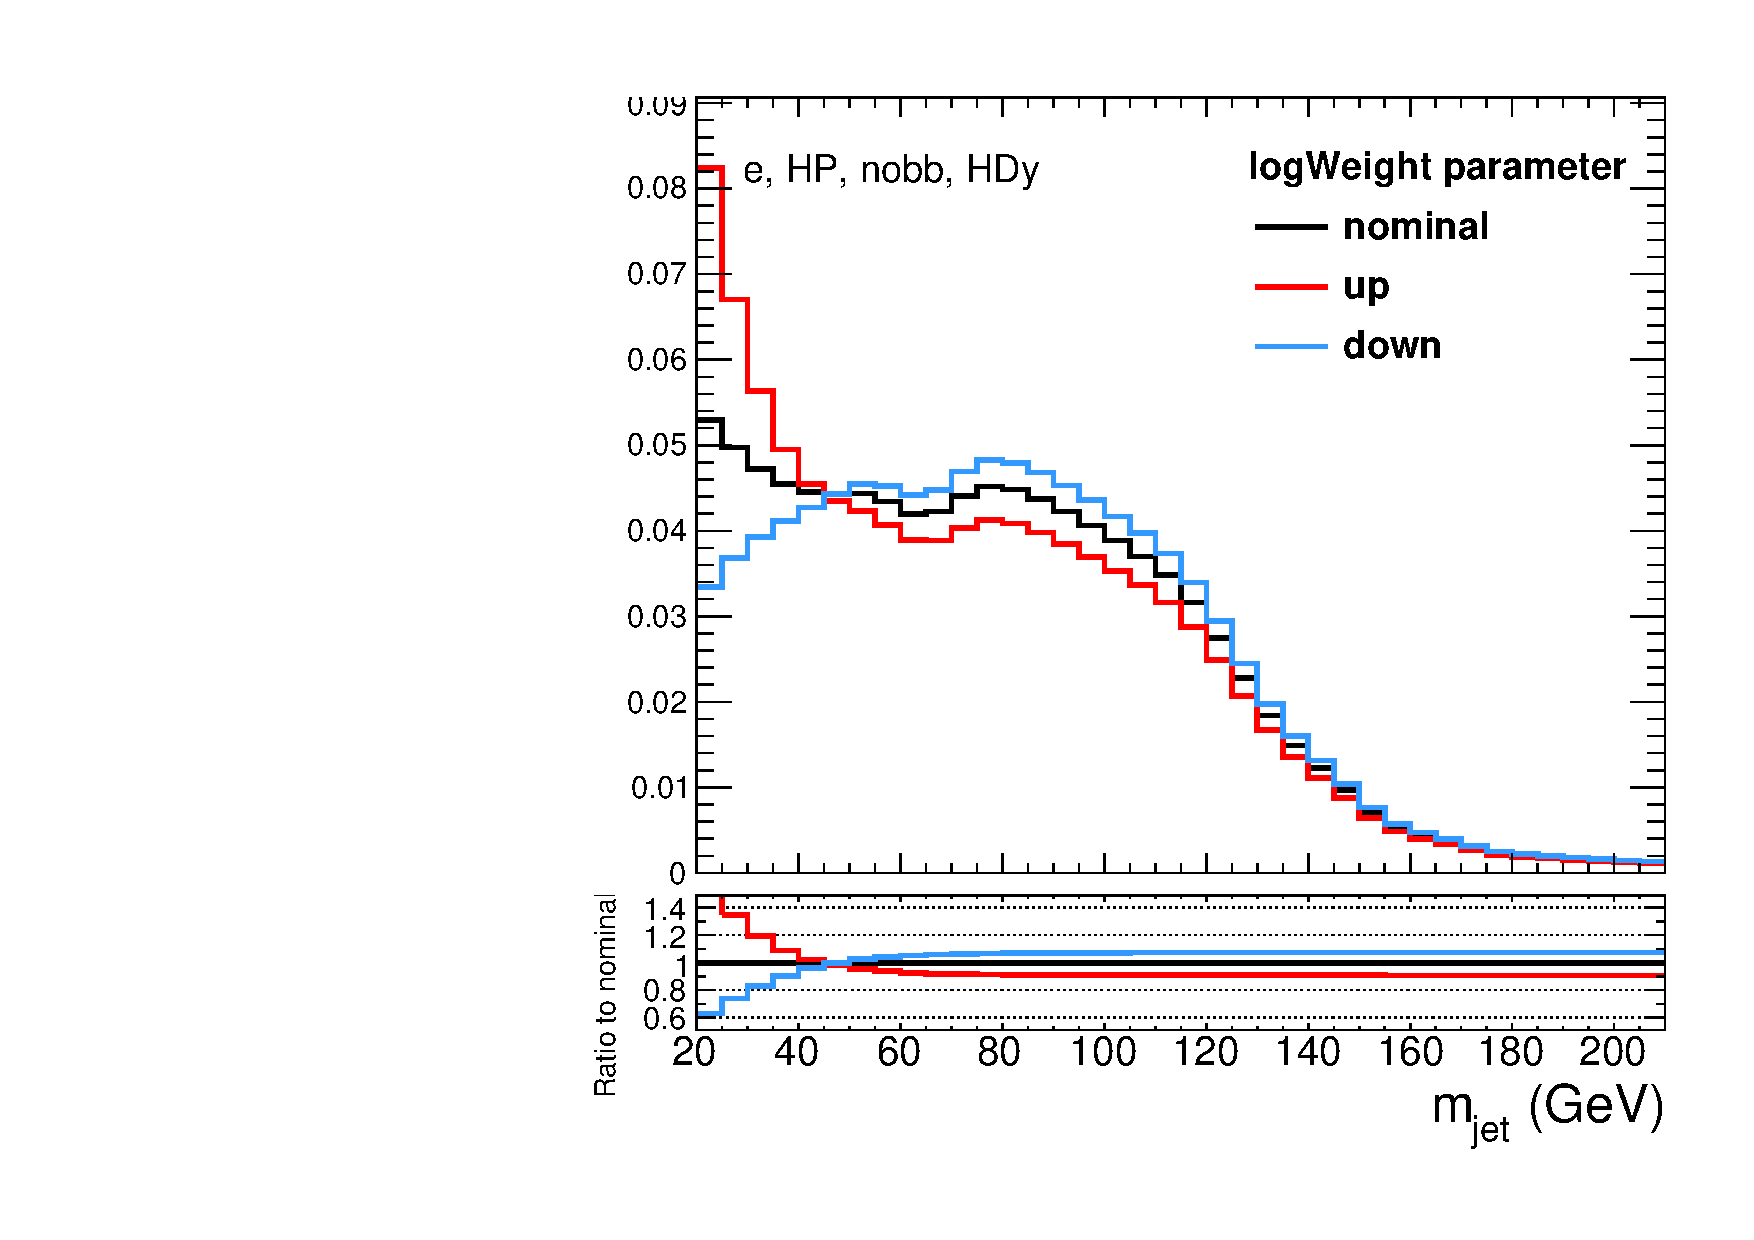
\includegraphics[width=0.21\textwidth]{fig/uncertainties/systs_nonRes_e_HP_nobb_HDy_logWeight_ProjY.pdf}
  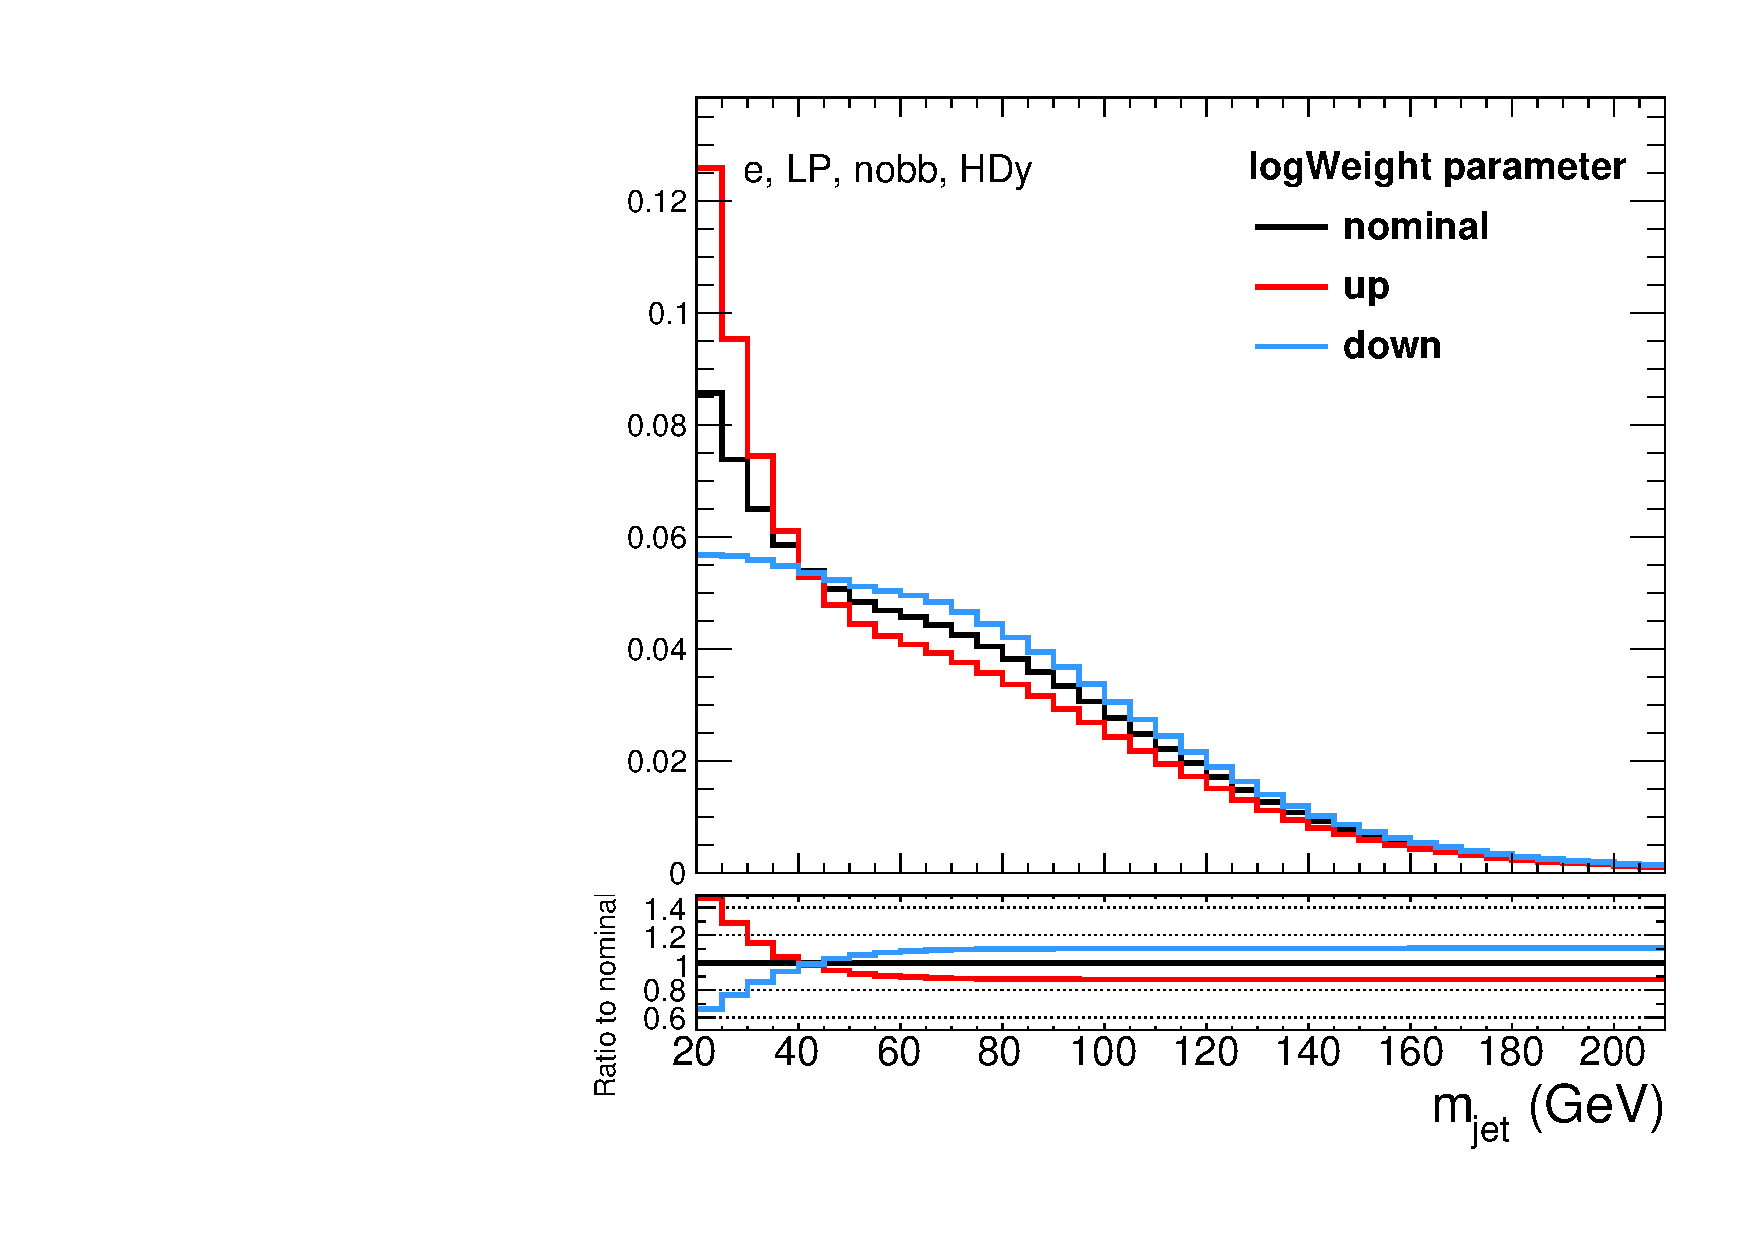
\includegraphics[width=0.21\textwidth]{fig/uncertainties/systs_nonRes_e_LP_nobb_HDy_logWeight_ProjY.pdf}\\
  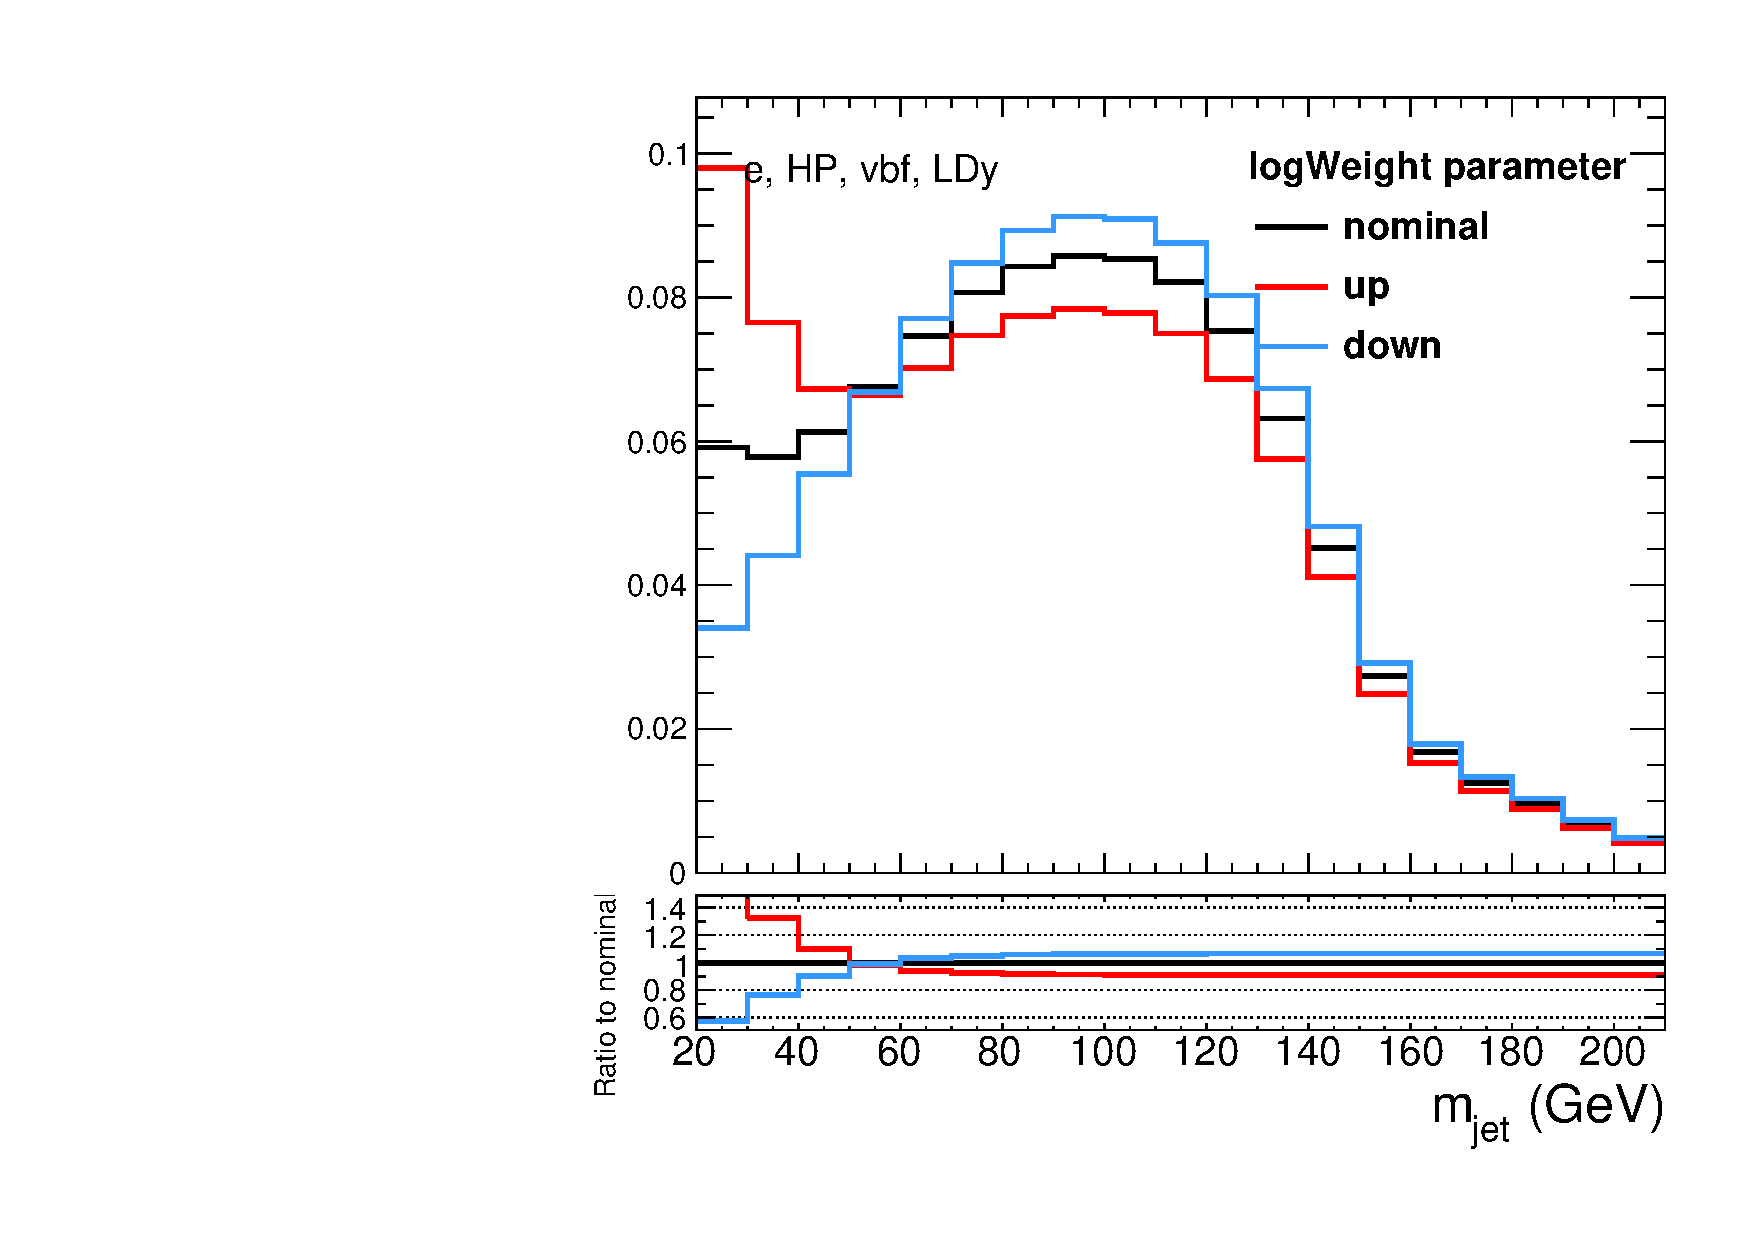
\includegraphics[width=0.21\textwidth]{fig/uncertainties/systs_nonRes_e_HP_vbf_LDy_logWeight_ProjY.pdf}
  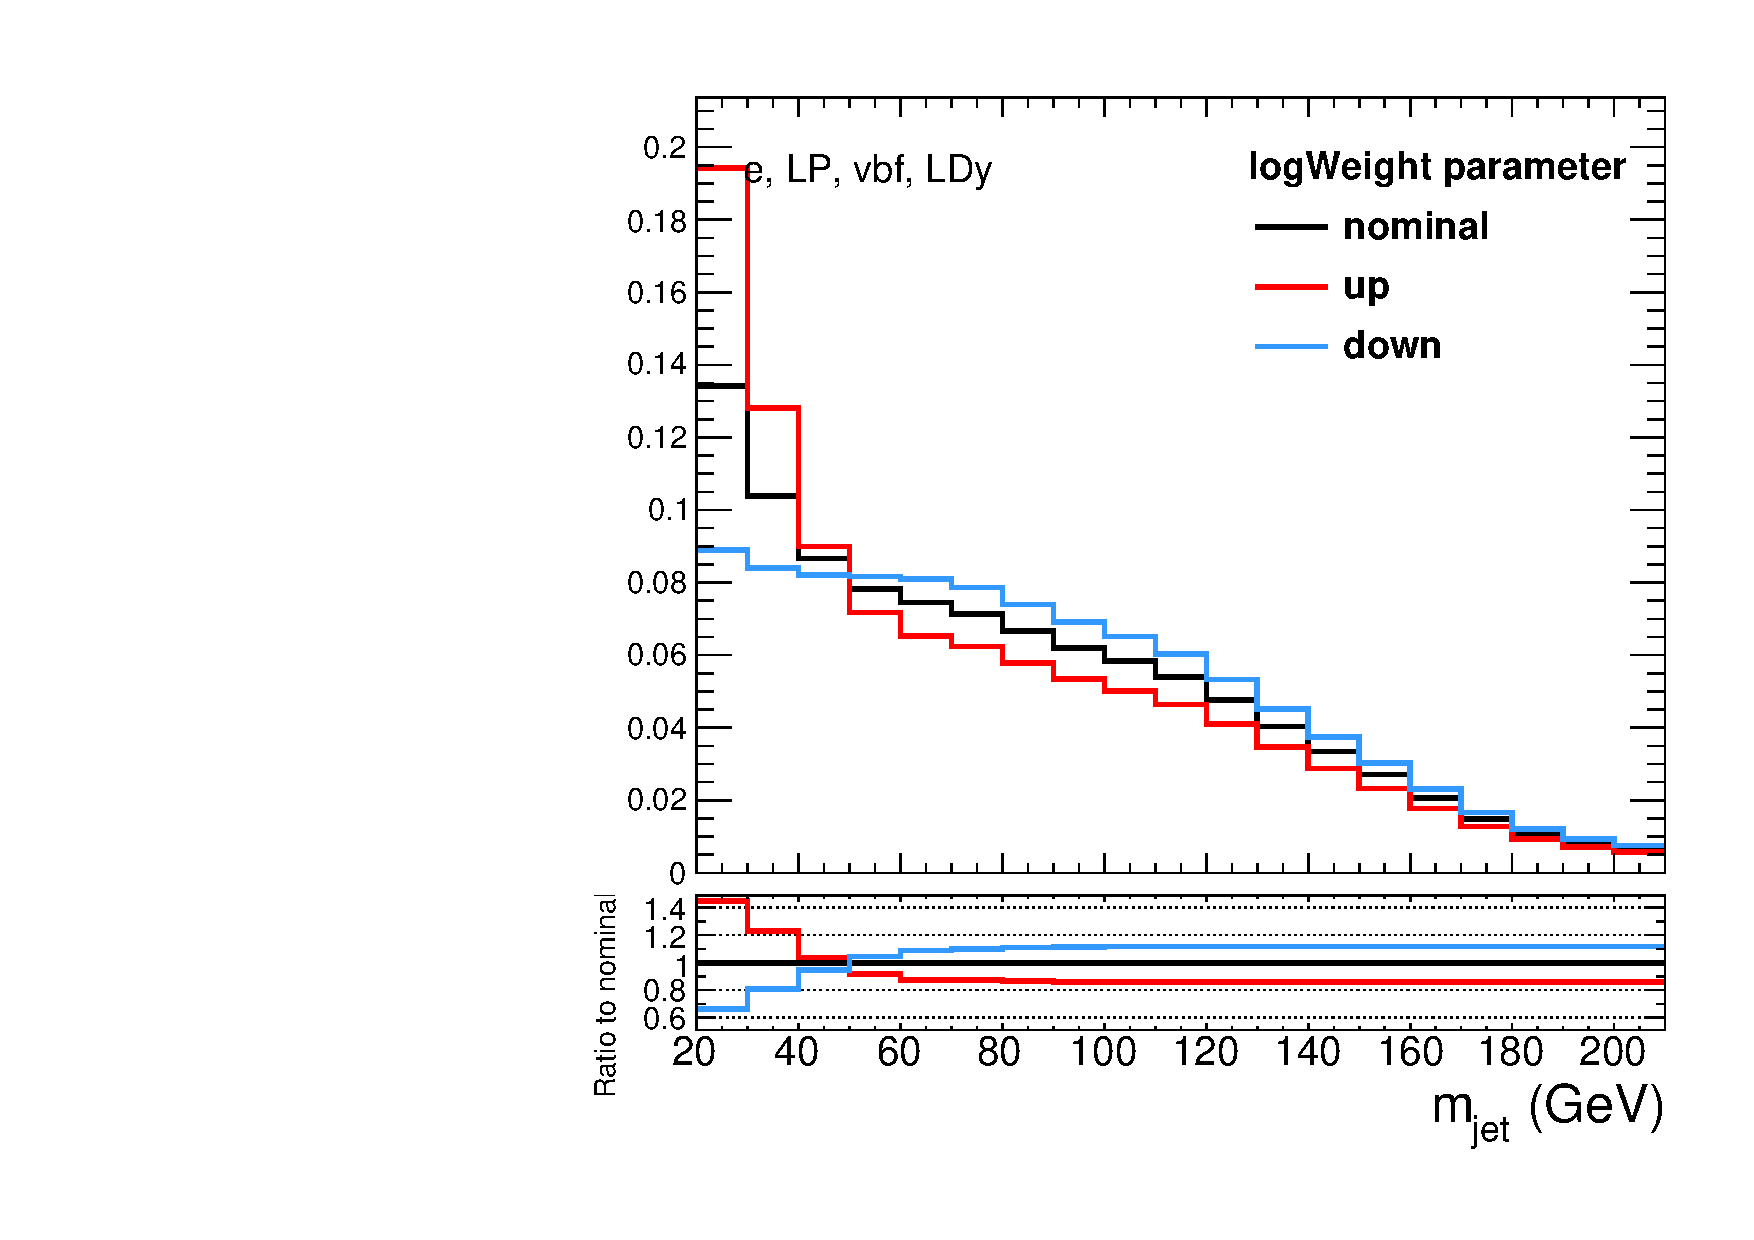
\includegraphics[width=0.21\textwidth]{fig/uncertainties/systs_nonRes_e_LP_vbf_LDy_logWeight_ProjY.pdf}
  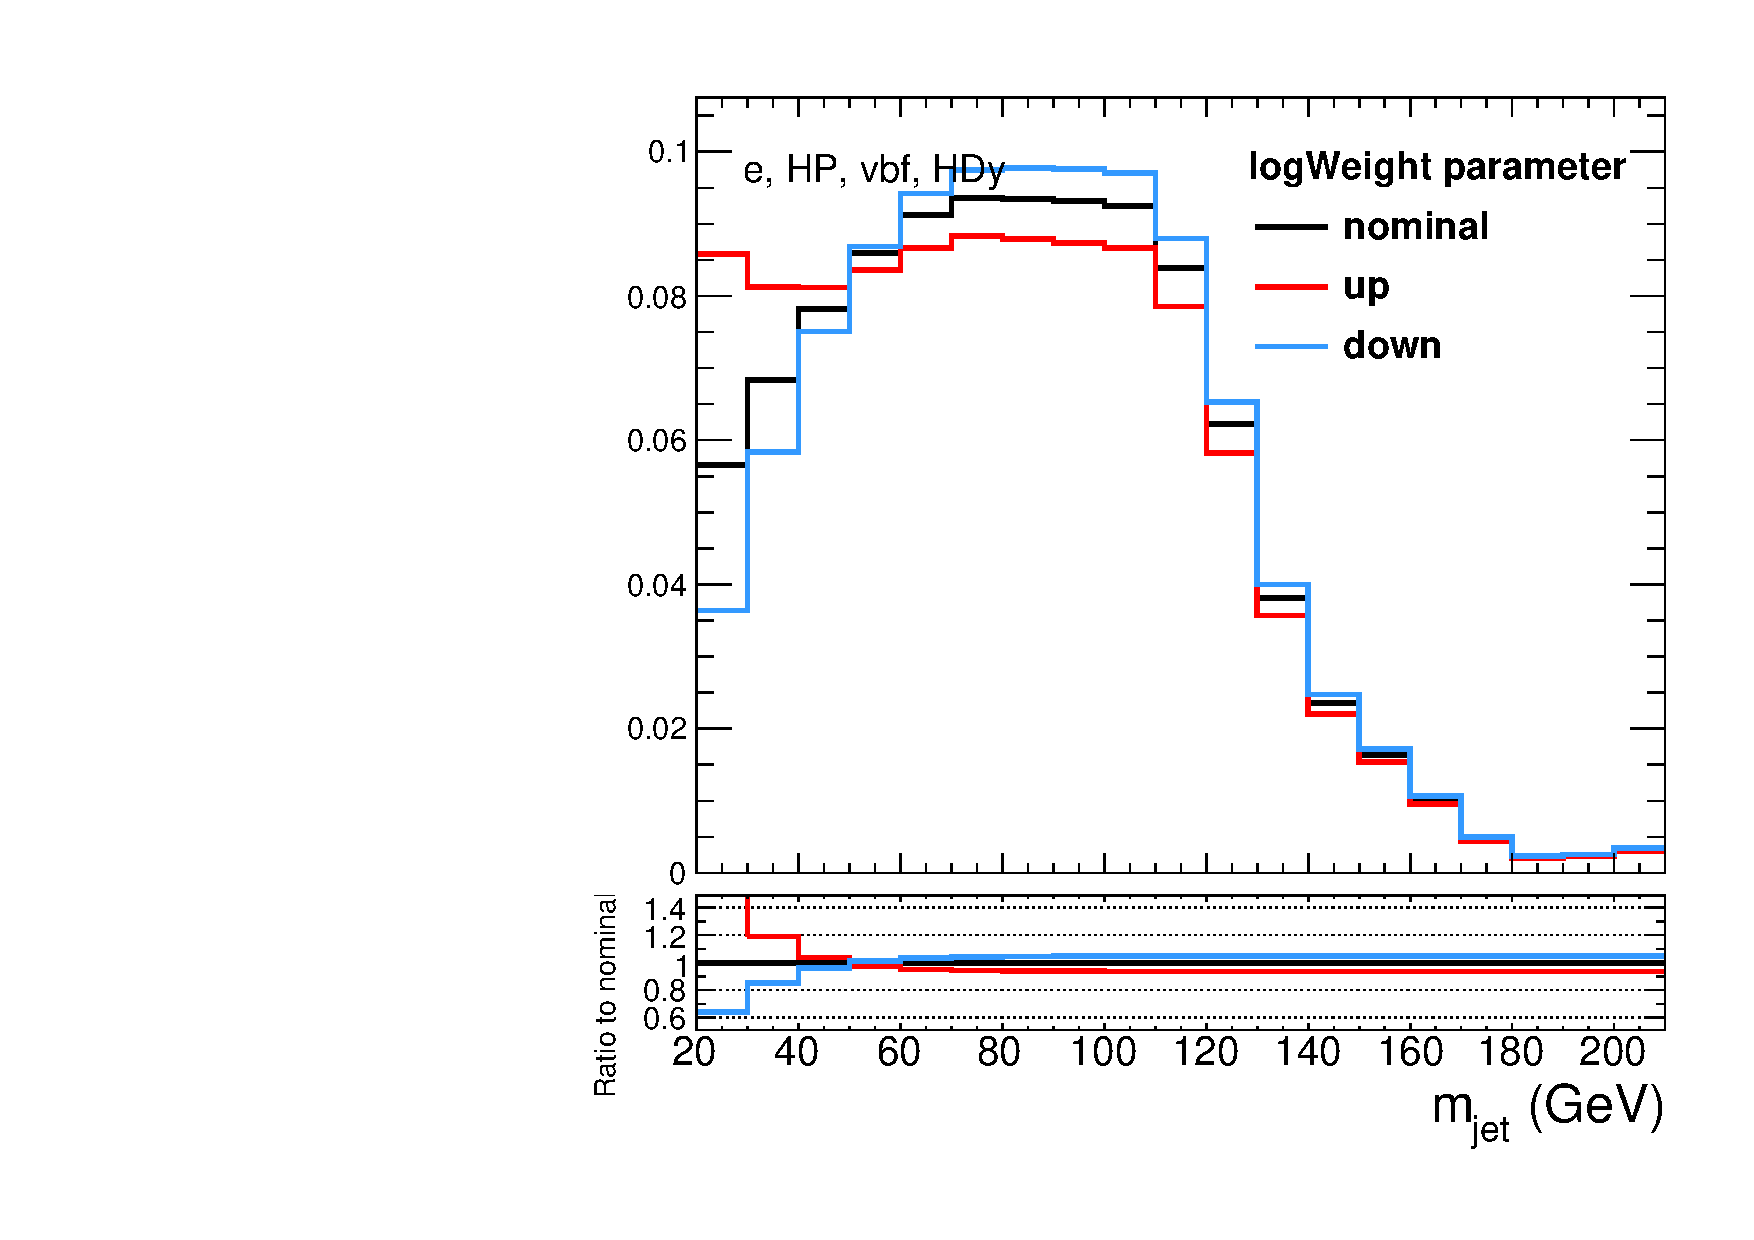
\includegraphics[width=0.21\textwidth]{fig/uncertainties/systs_nonRes_e_HP_vbf_HDy_logWeight_ProjY.pdf}
  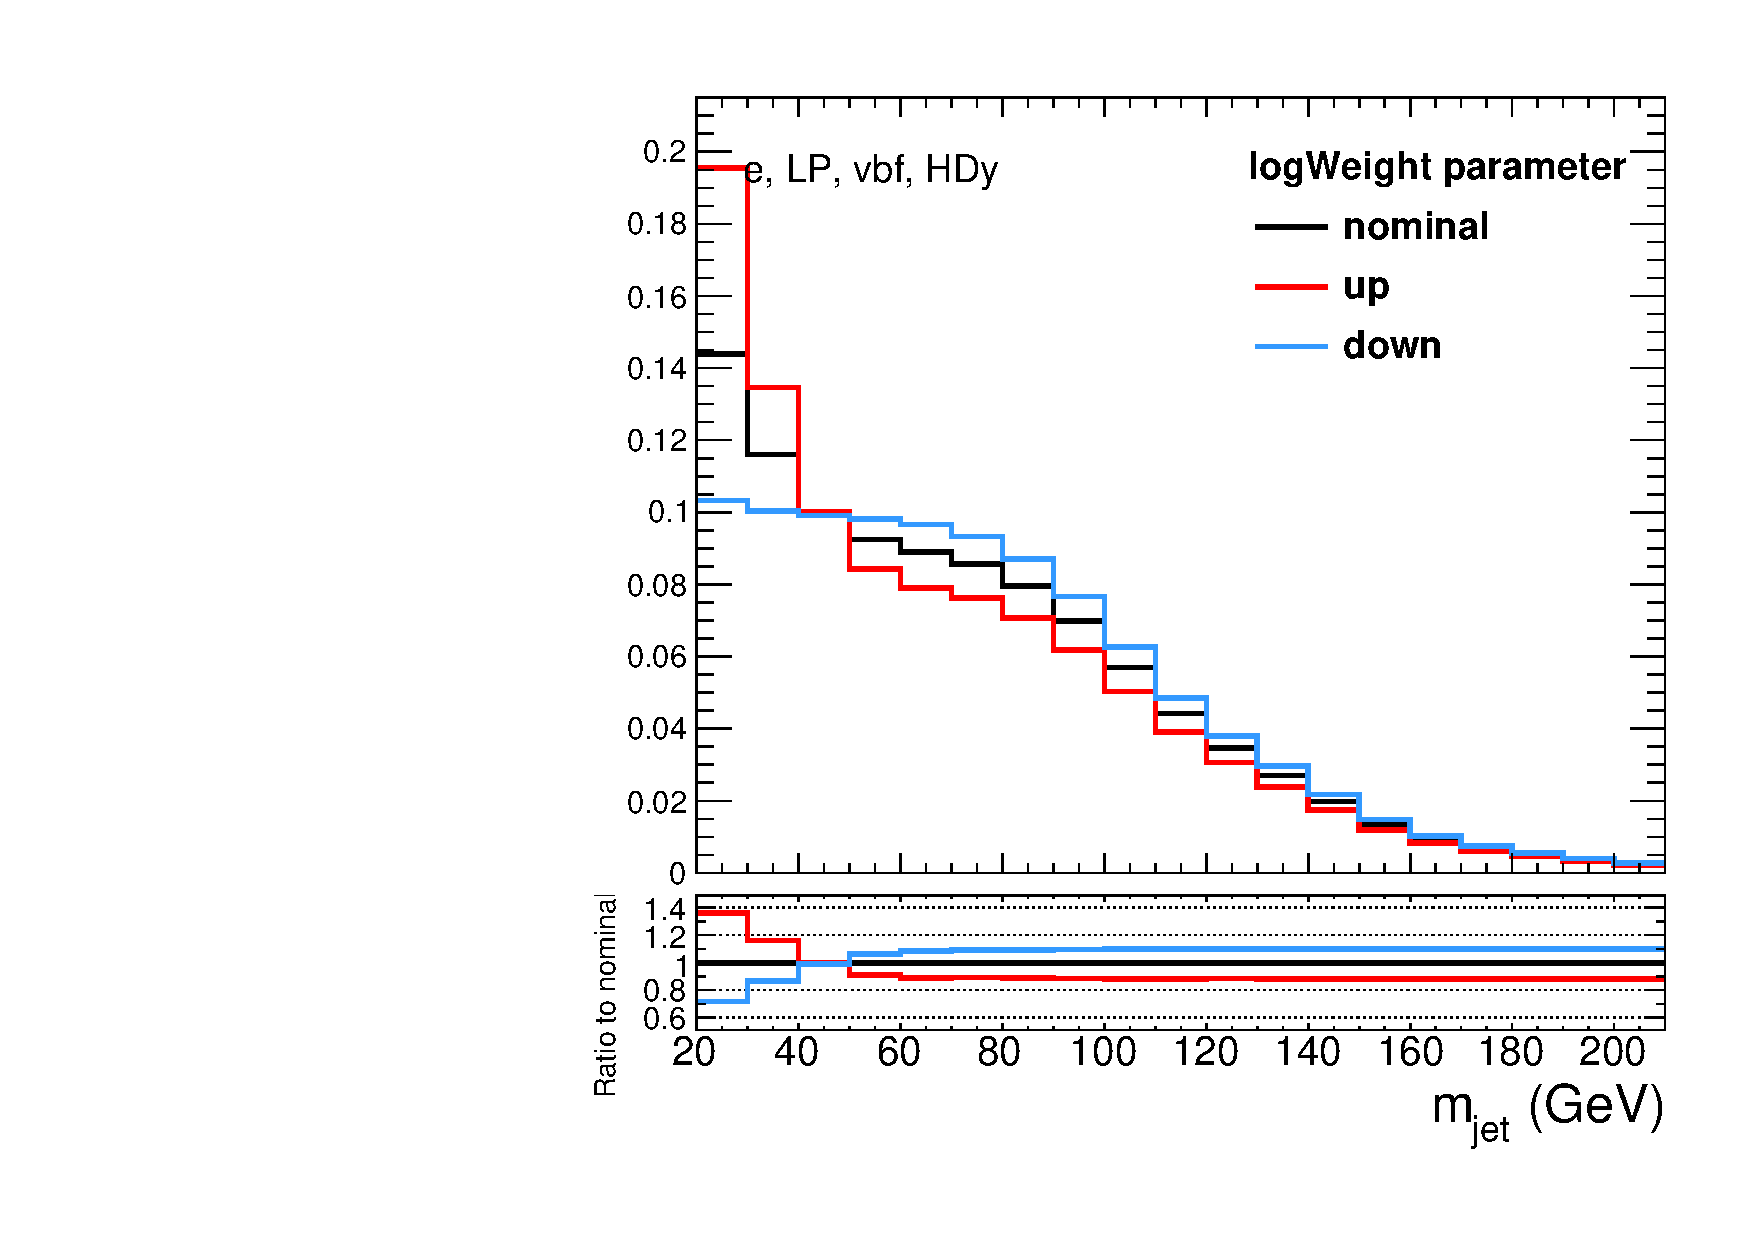
\includegraphics[width=0.21\textwidth]{fig/uncertainties/systs_nonRes_e_LP_vbf_HDy_logWeight_ProjY.pdf}\\
  \caption{
    Projections of the nominal and alternative shapes of the non-resonant background onto the \MJ dimension obtained from applying $\pm3\sigma$ variations of the logWeight uncertainties for the electron channel.
    Columns 1 to 4: HP-LDy, LP-LDy, HP-HDy, LP-HDy.
    Rows 1 to 3: bb, nobb, vbf.
  }
  \label{fig:systNonResMJ_logWeight}
\end{figure}

\begin{figure}[htbp]
  \centering
  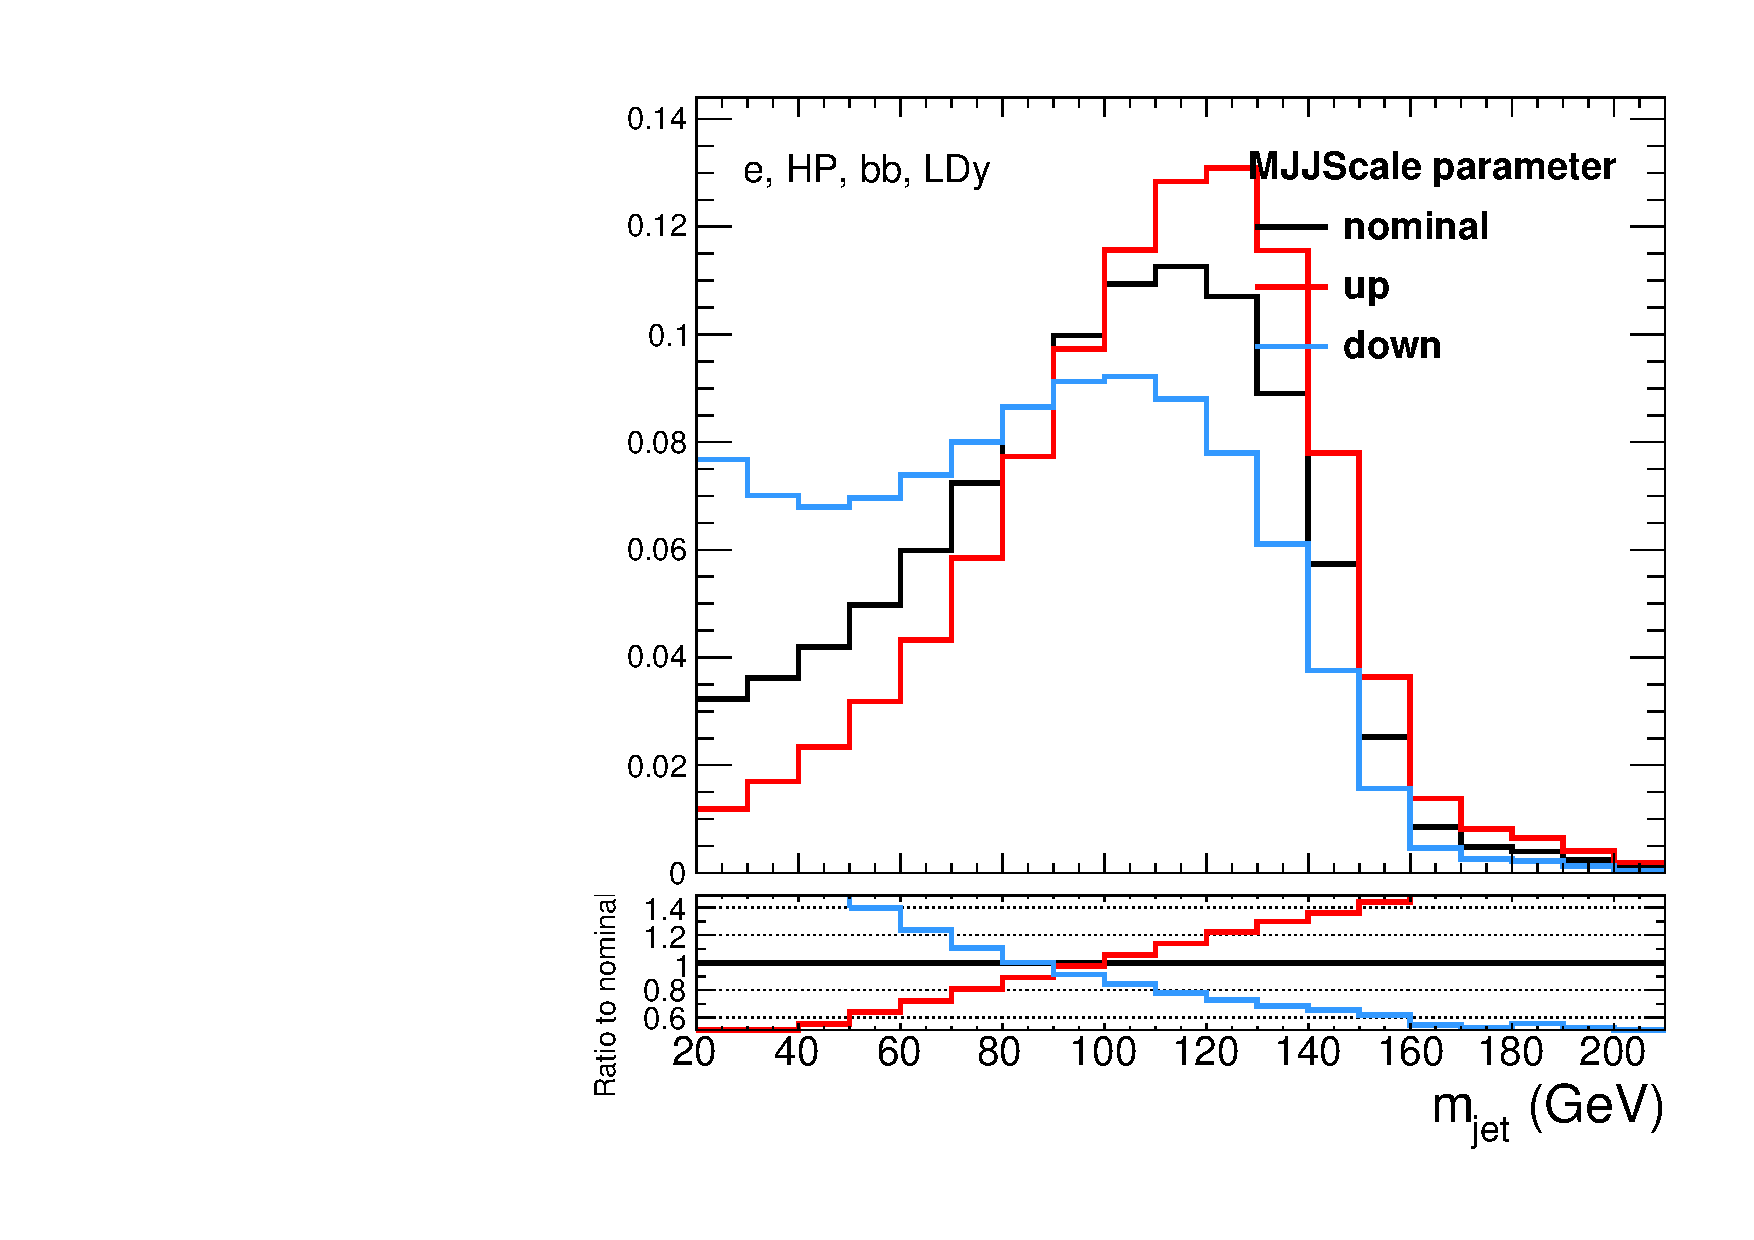
\includegraphics[width=0.21\textwidth]{fig/uncertainties/systs_nonRes_e_HP_bb_LDy_MJJScale_ProjY.pdf}
  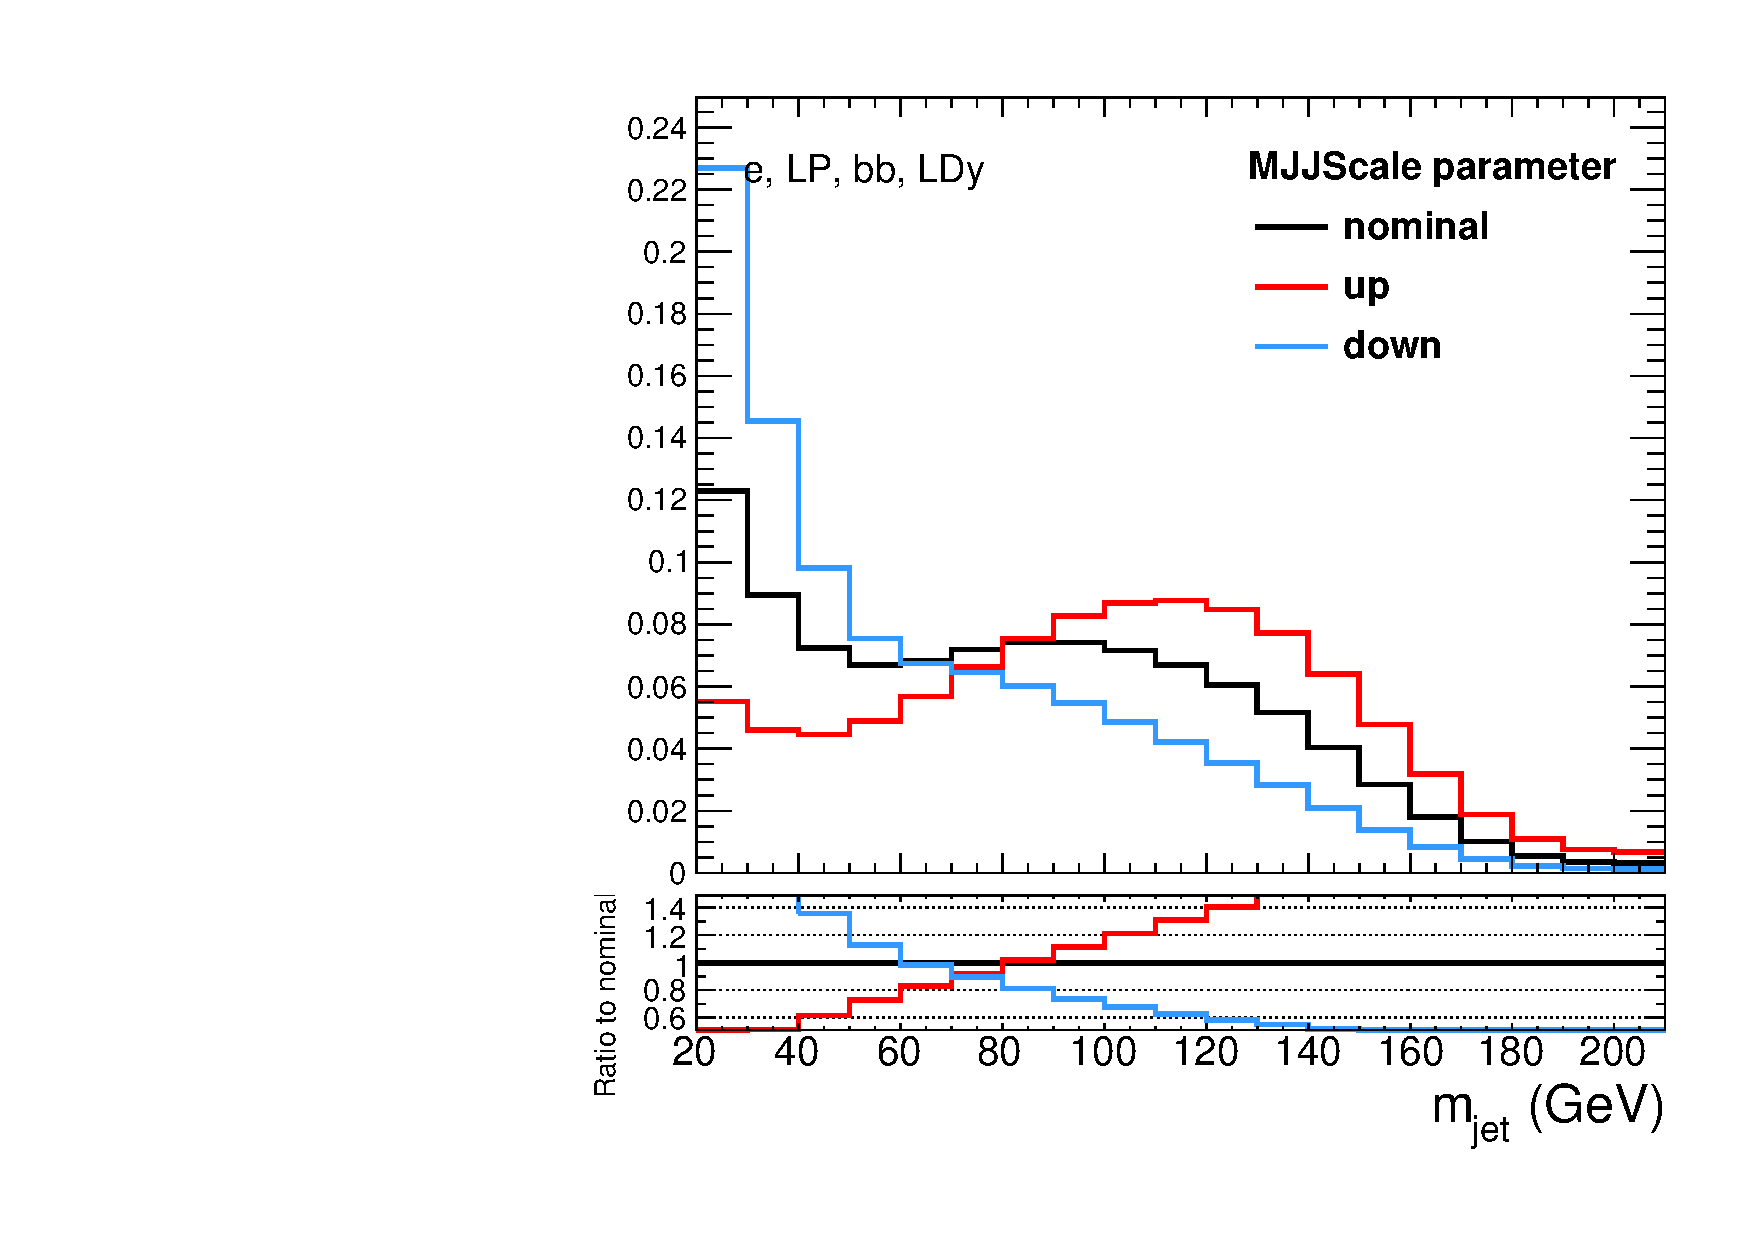
\includegraphics[width=0.21\textwidth]{fig/uncertainties/systs_nonRes_e_LP_bb_LDy_MJJScale_ProjY.pdf}
  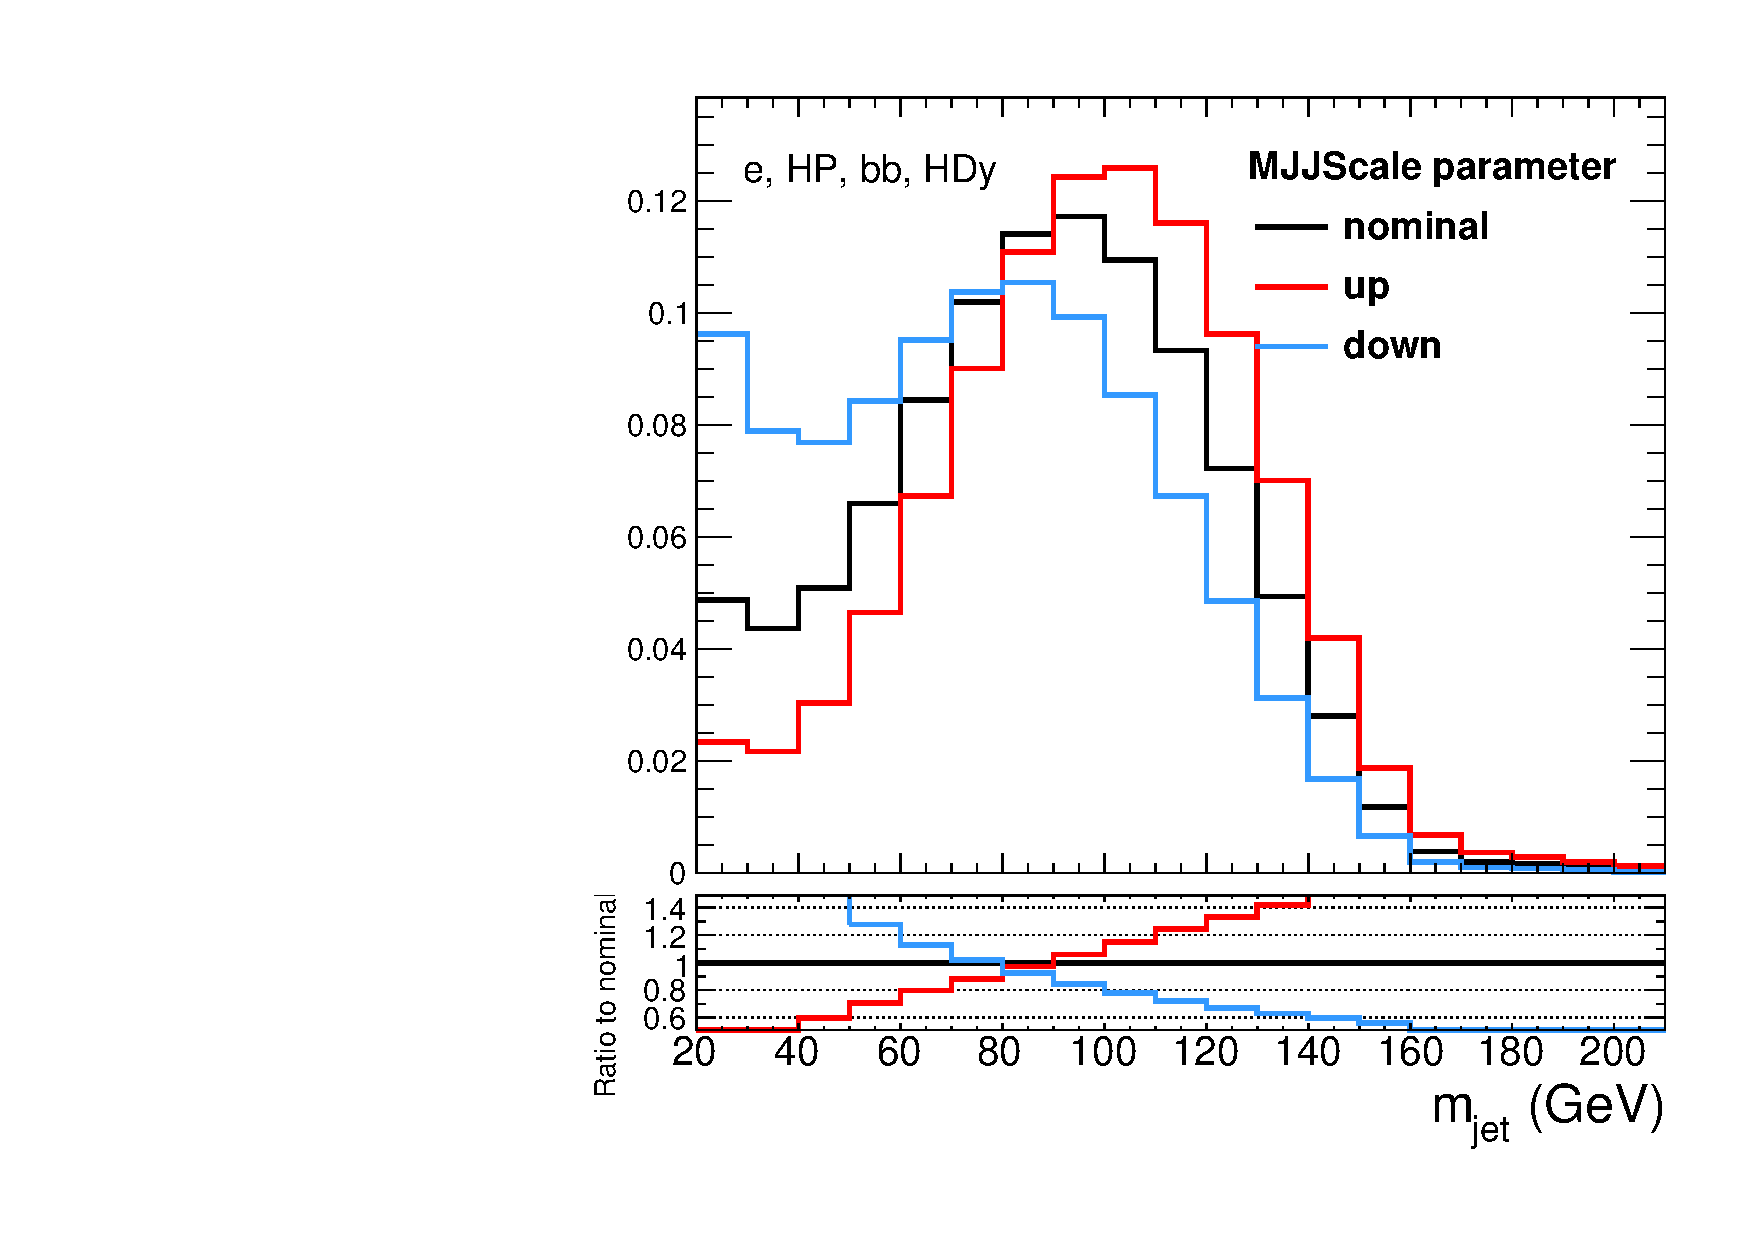
\includegraphics[width=0.21\textwidth]{fig/uncertainties/systs_nonRes_e_HP_bb_HDy_MJJScale_ProjY.pdf}
  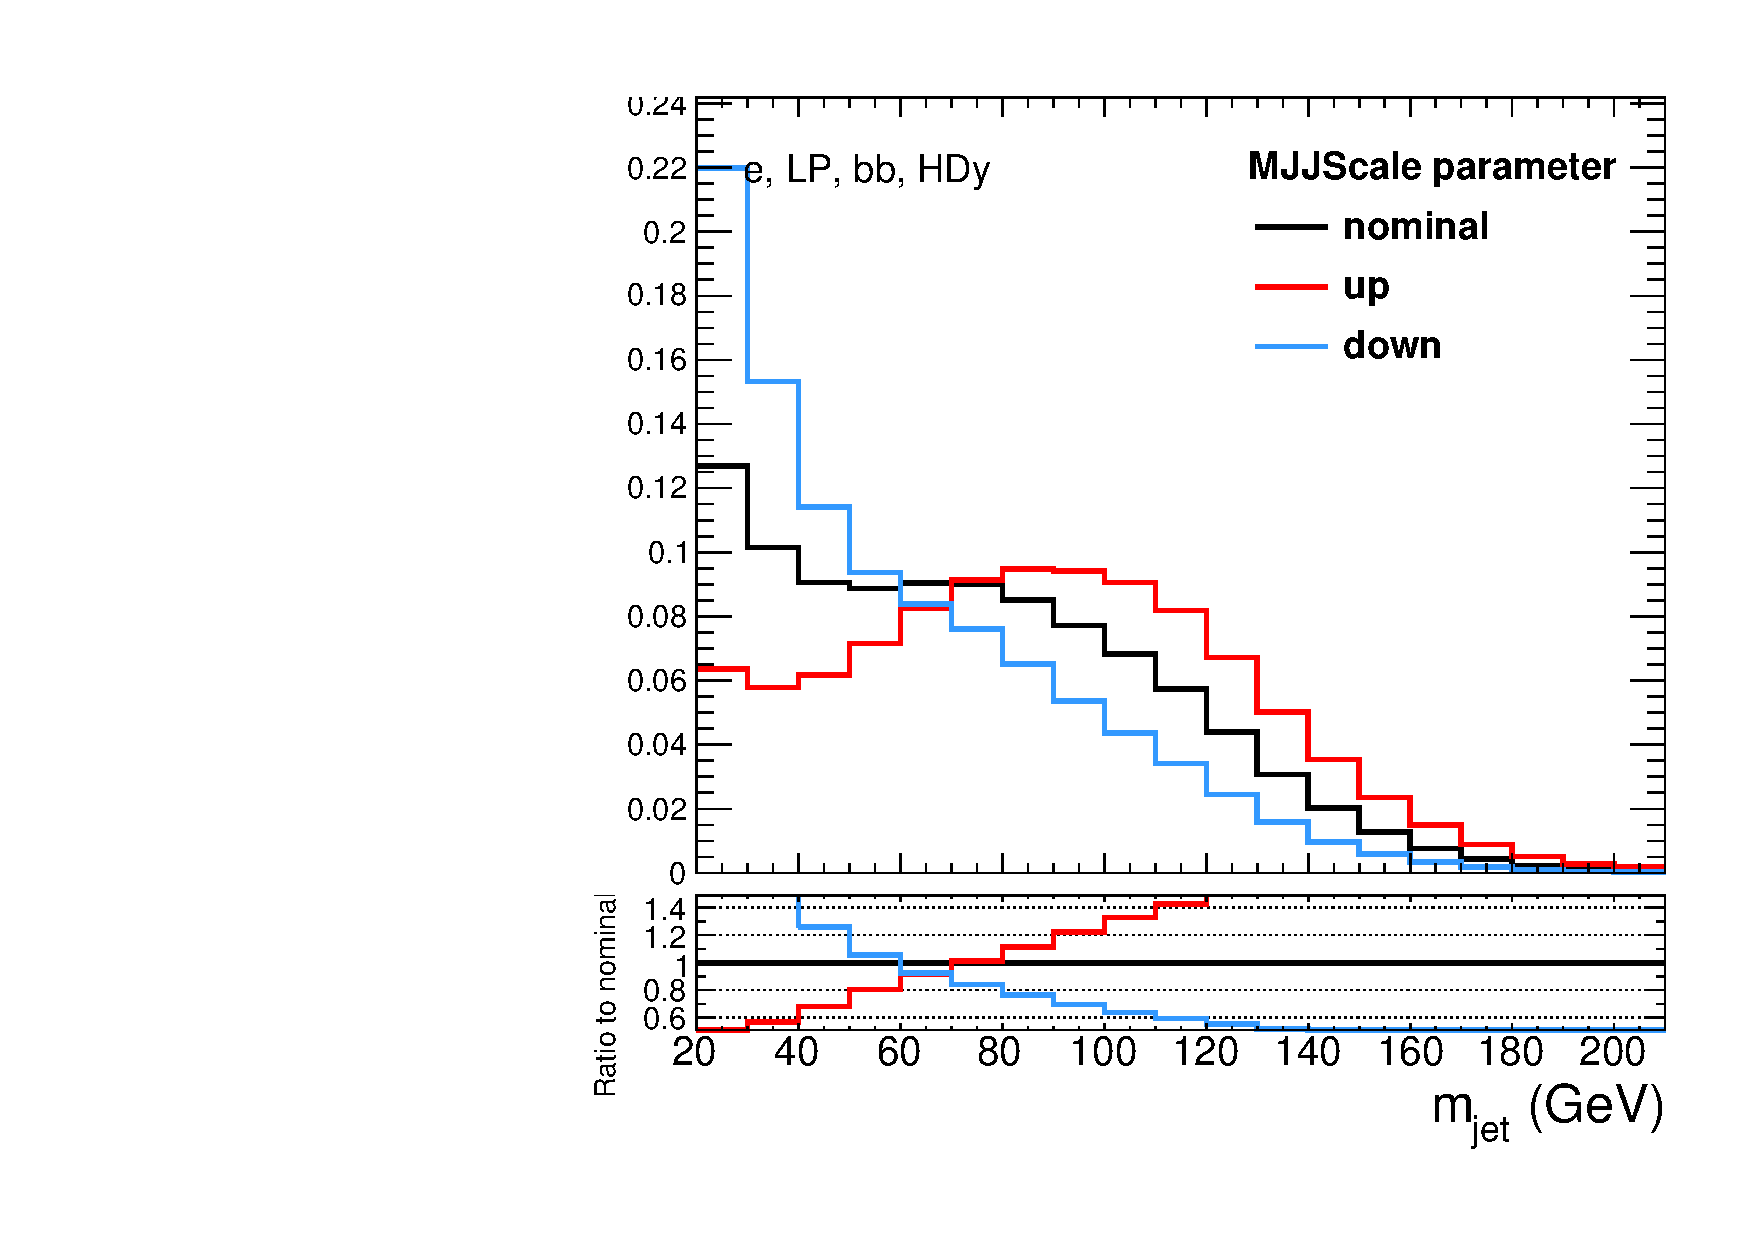
\includegraphics[width=0.21\textwidth]{fig/uncertainties/systs_nonRes_e_LP_bb_HDy_MJJScale_ProjY.pdf}\\
  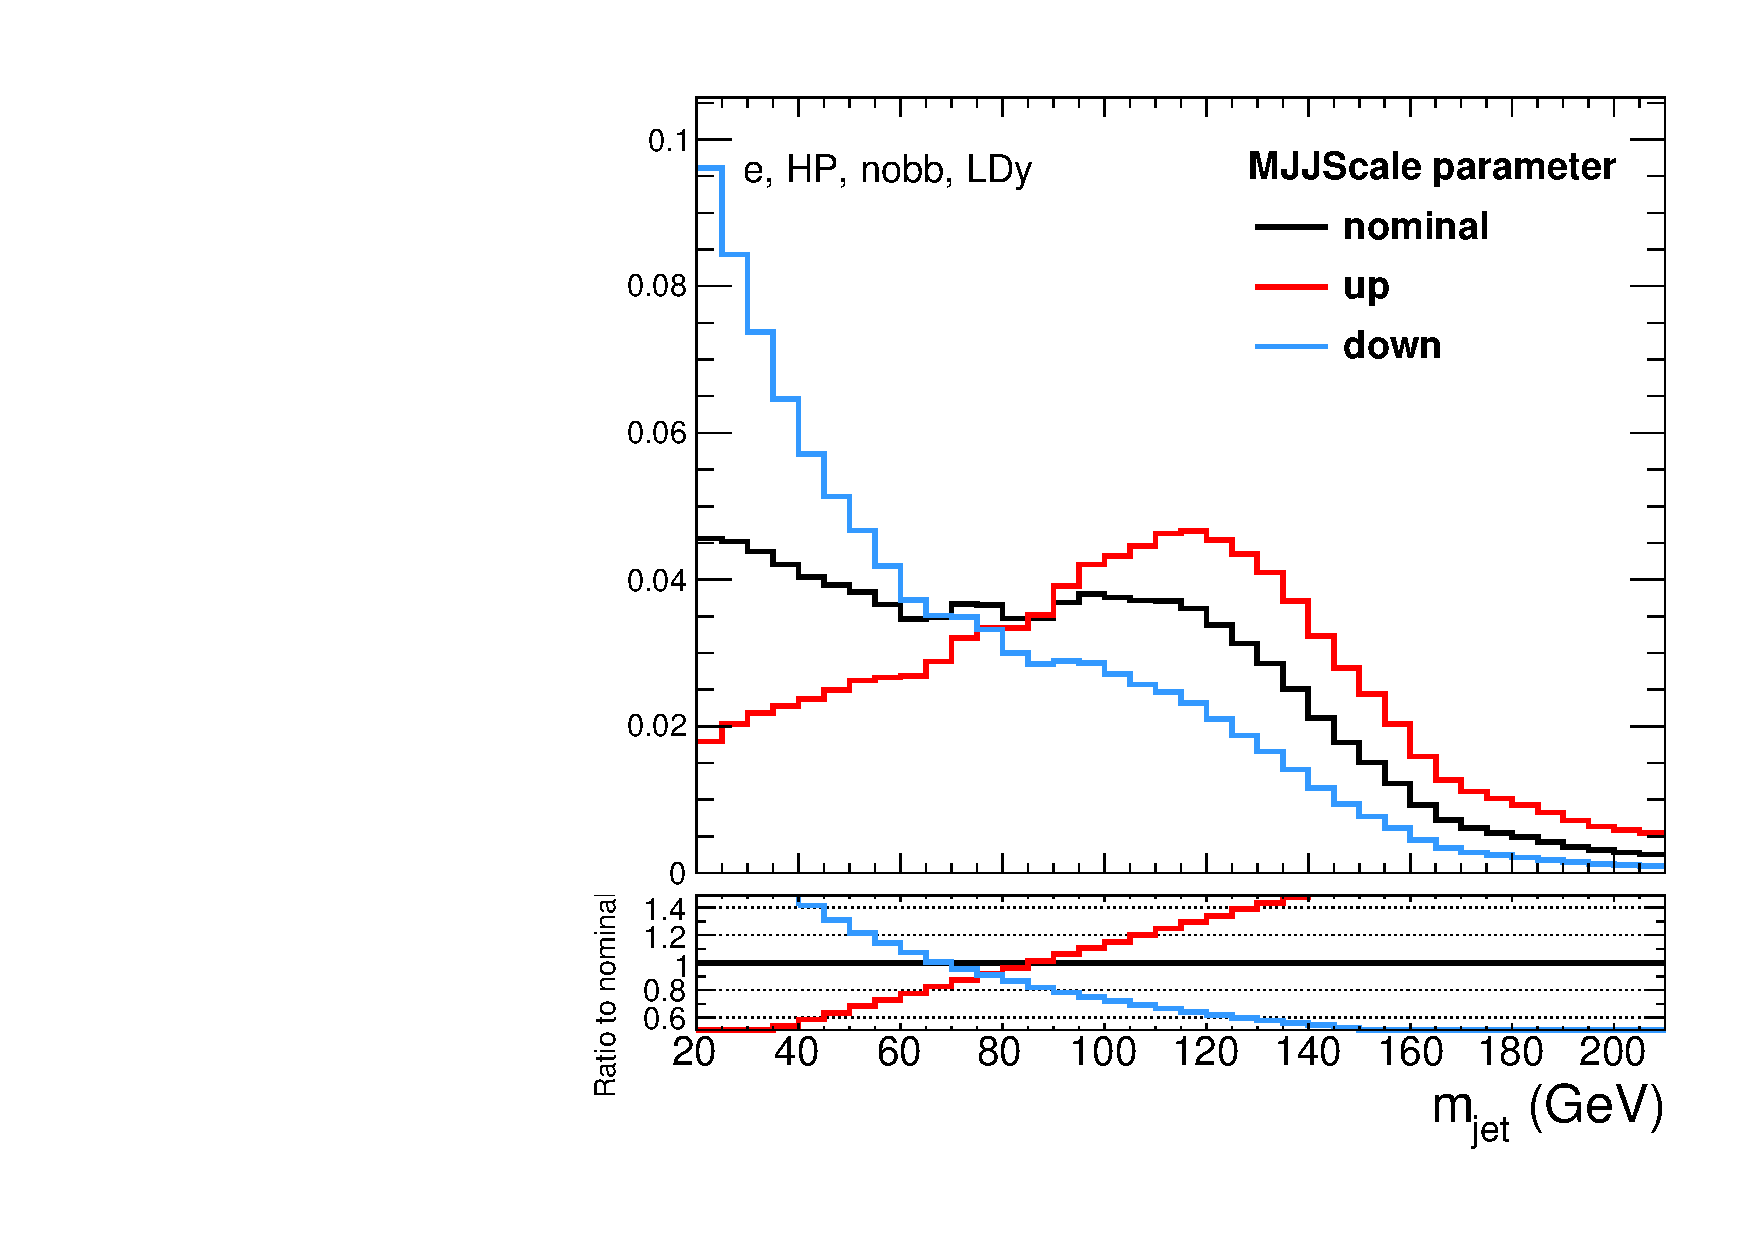
\includegraphics[width=0.21\textwidth]{fig/uncertainties/systs_nonRes_e_HP_nobb_LDy_MJJScale_ProjY.pdf}
  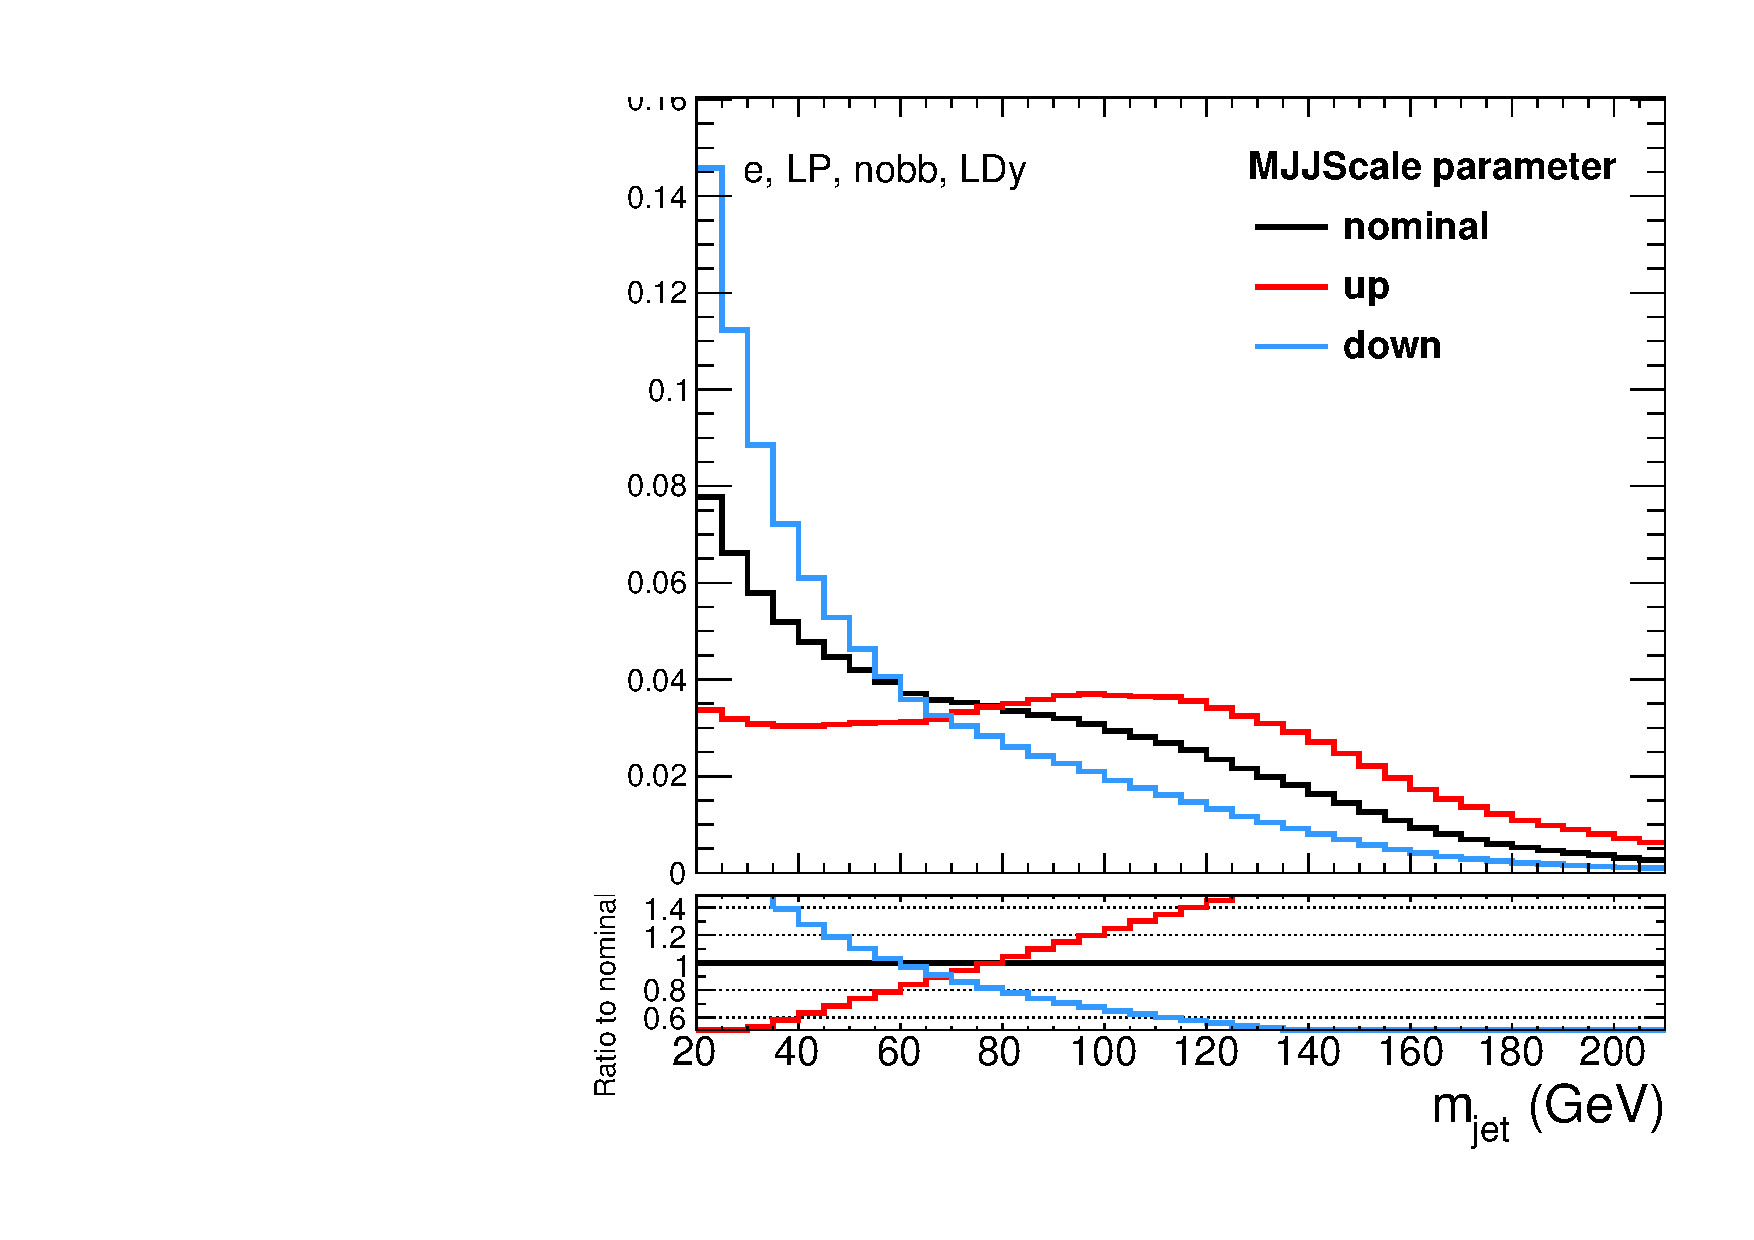
\includegraphics[width=0.21\textwidth]{fig/uncertainties/systs_nonRes_e_LP_nobb_LDy_MJJScale_ProjY.pdf}
  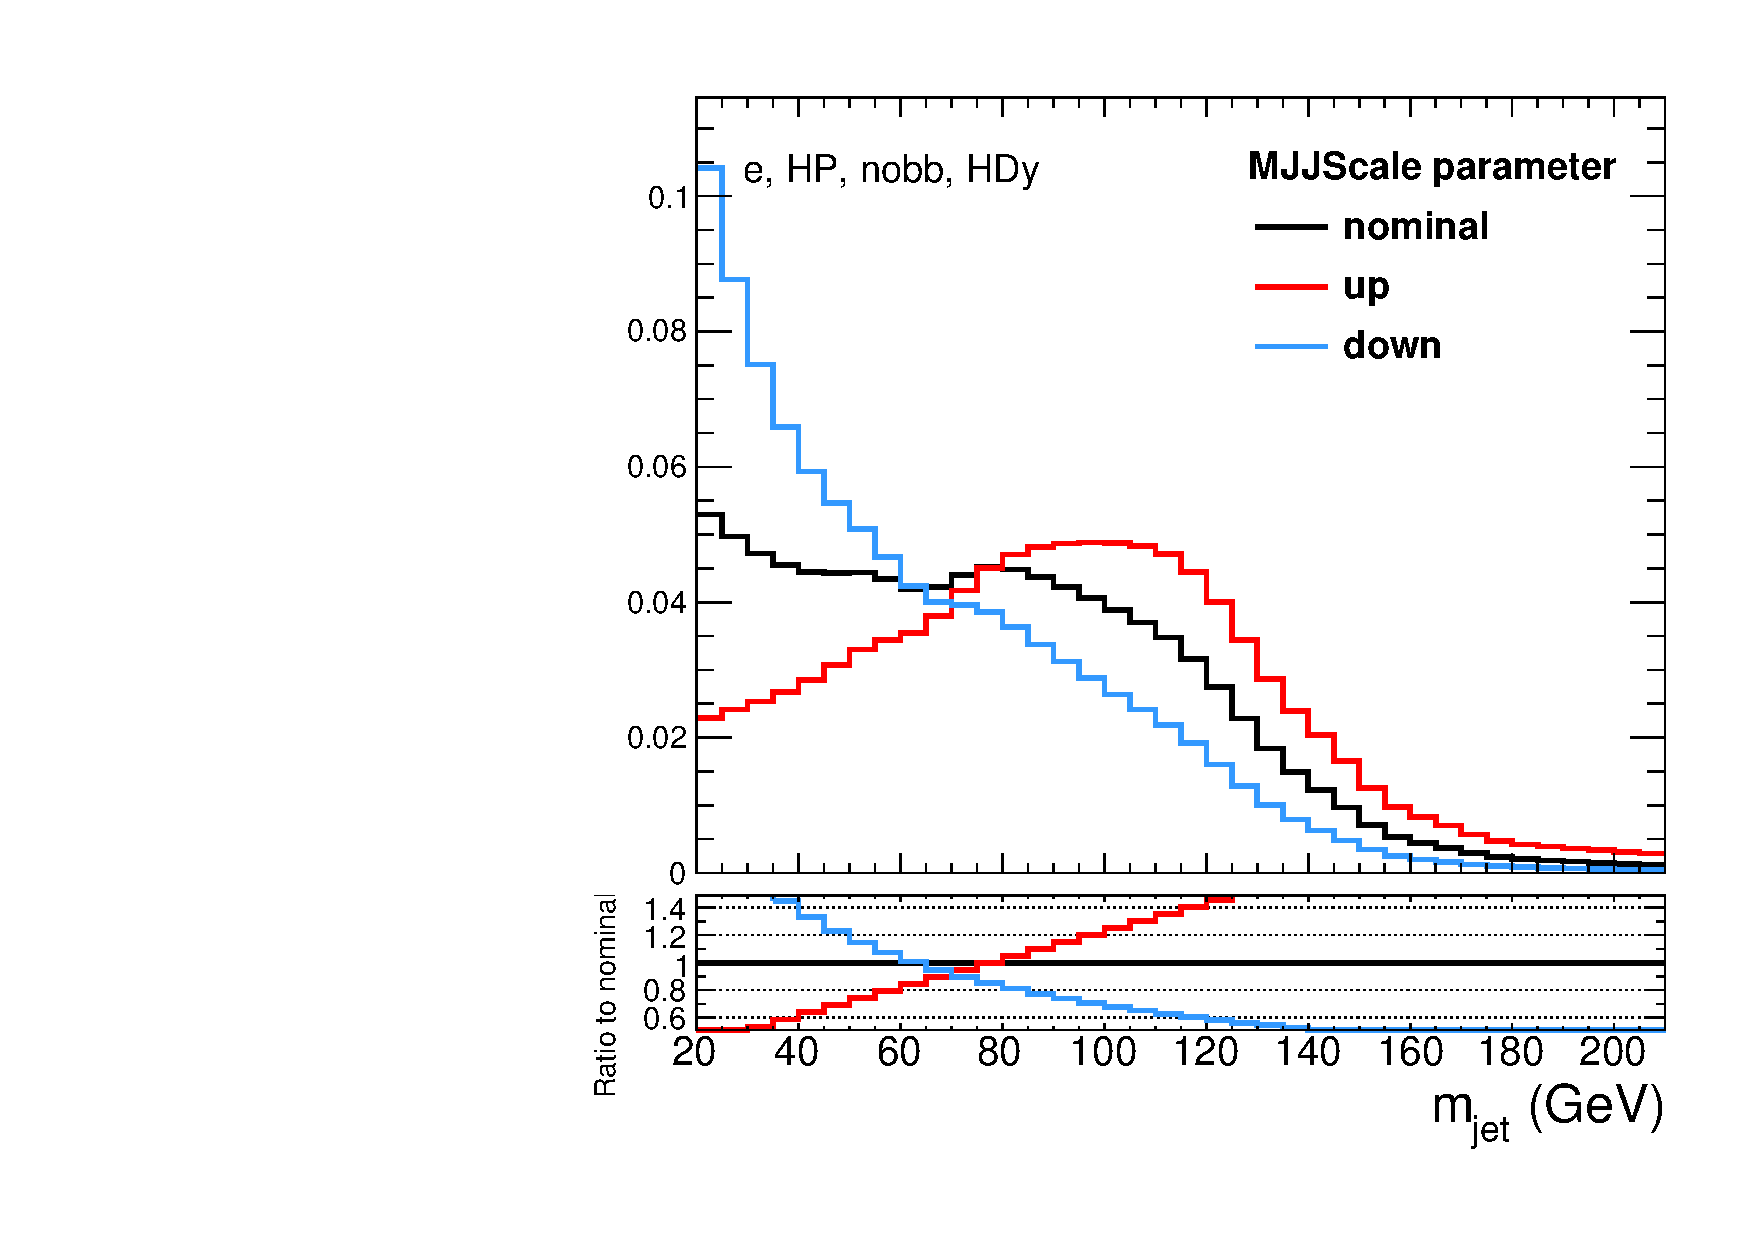
\includegraphics[width=0.21\textwidth]{fig/uncertainties/systs_nonRes_e_HP_nobb_HDy_MJJScale_ProjY.pdf}
  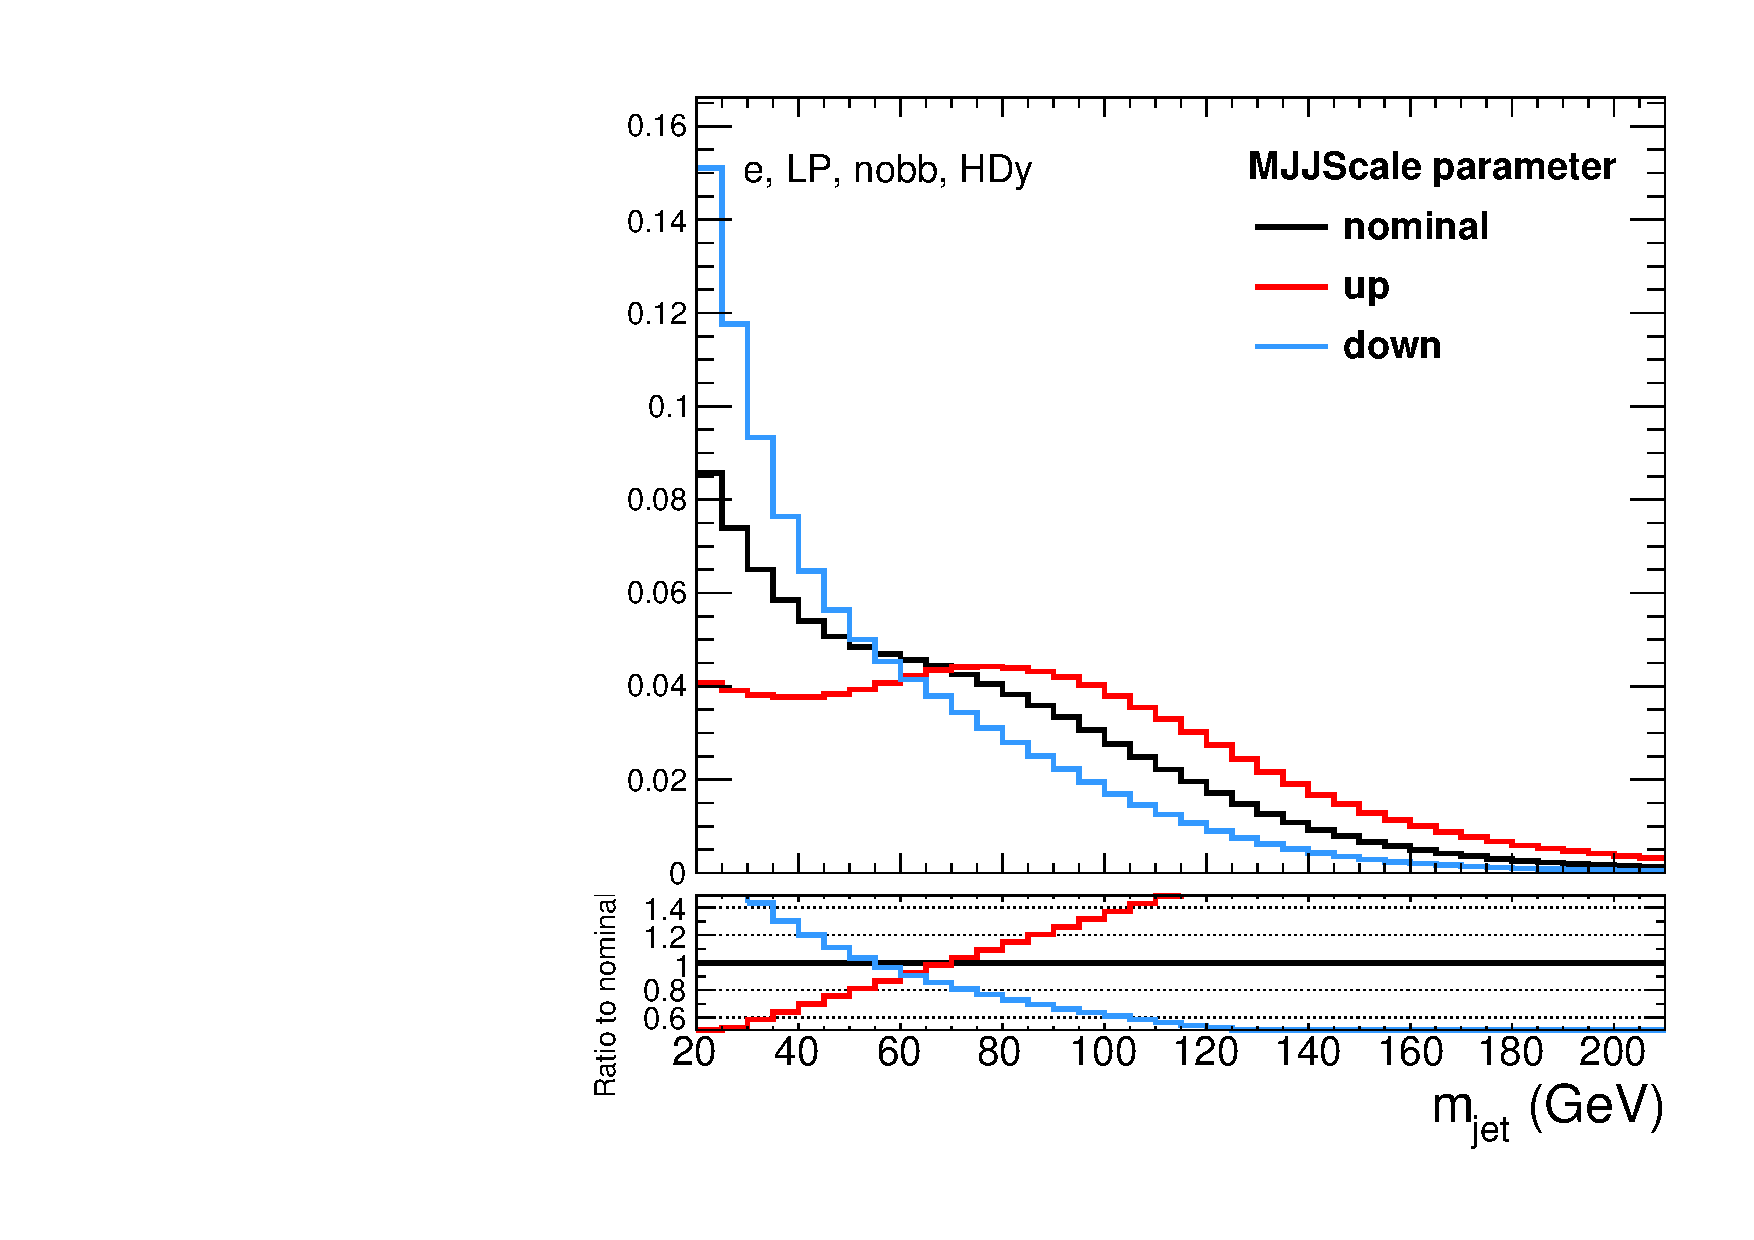
\includegraphics[width=0.21\textwidth]{fig/uncertainties/systs_nonRes_e_LP_nobb_HDy_MJJScale_ProjY.pdf}\\
  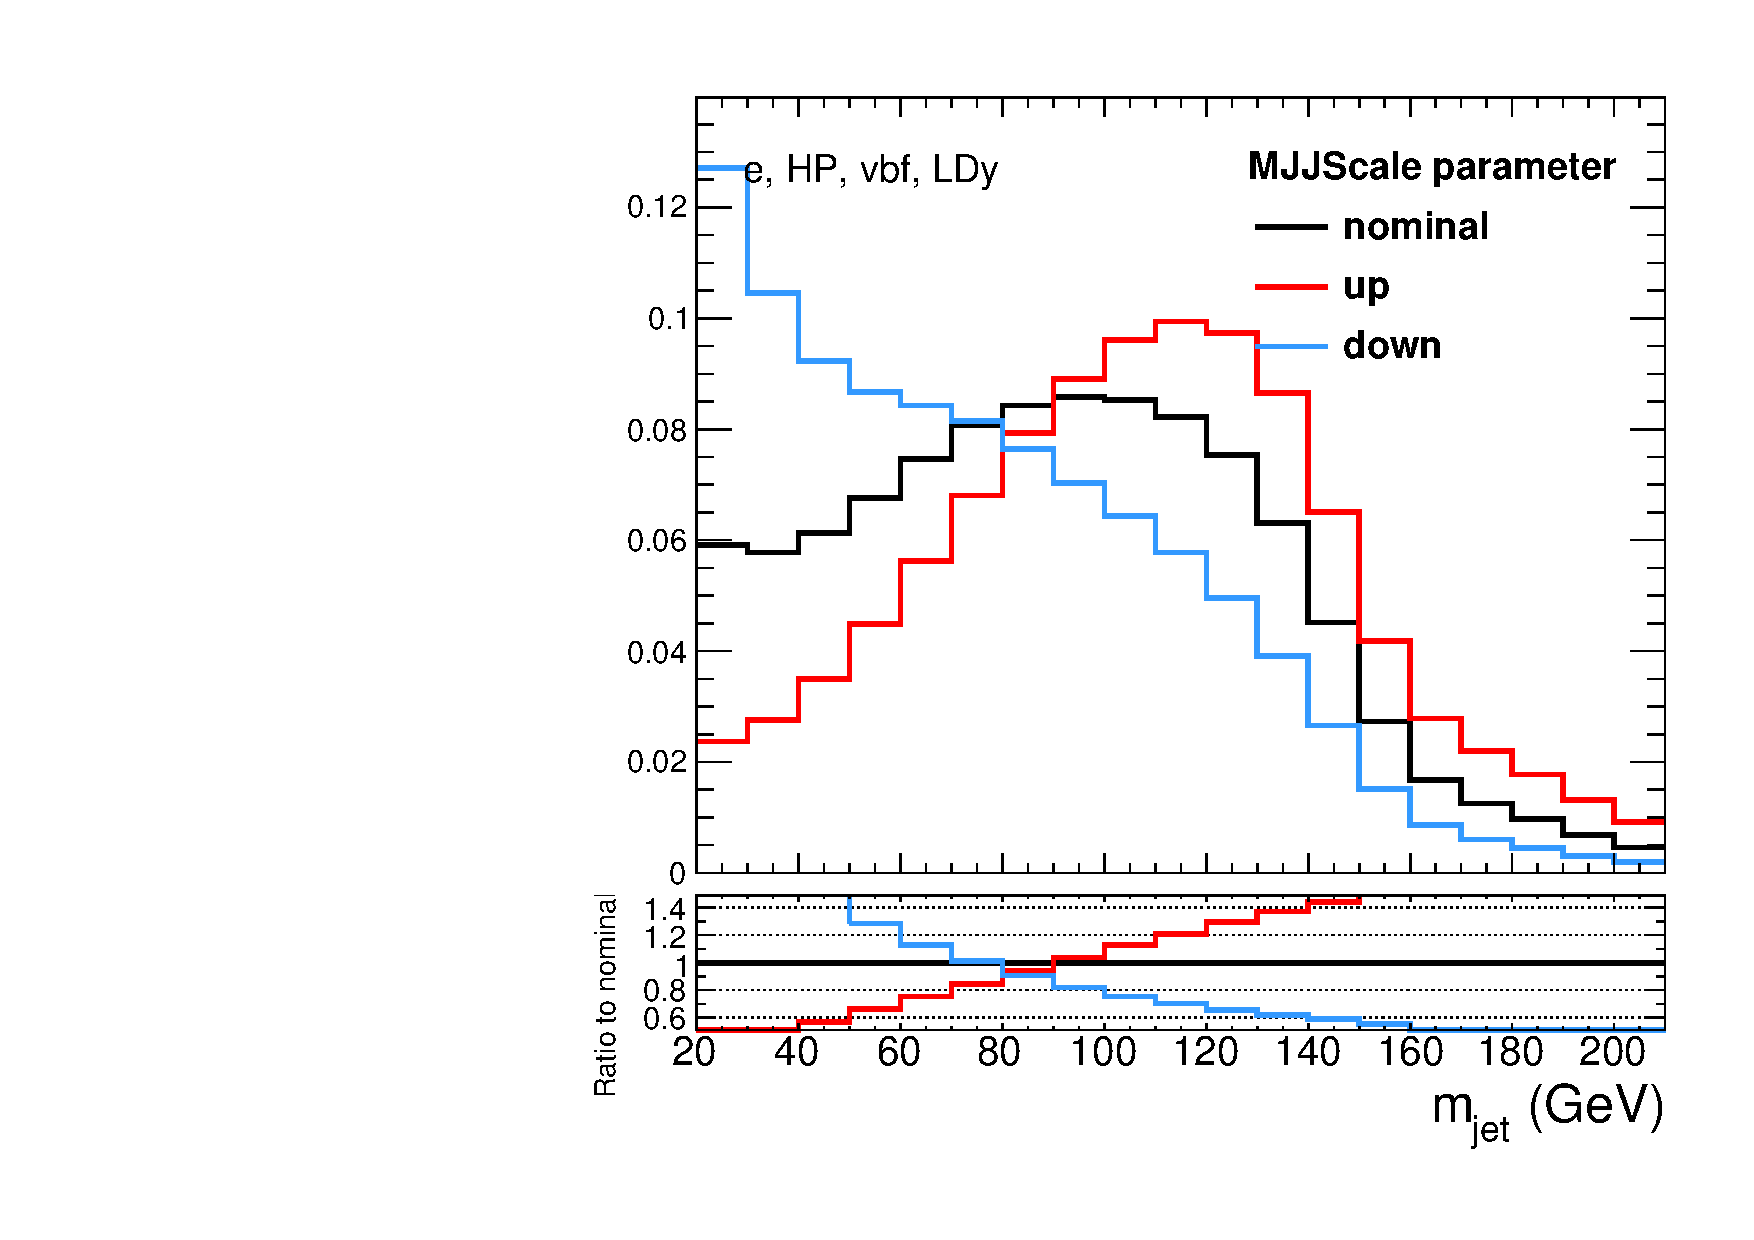
\includegraphics[width=0.21\textwidth]{fig/uncertainties/systs_nonRes_e_HP_vbf_LDy_MJJScale_ProjY.pdf}
  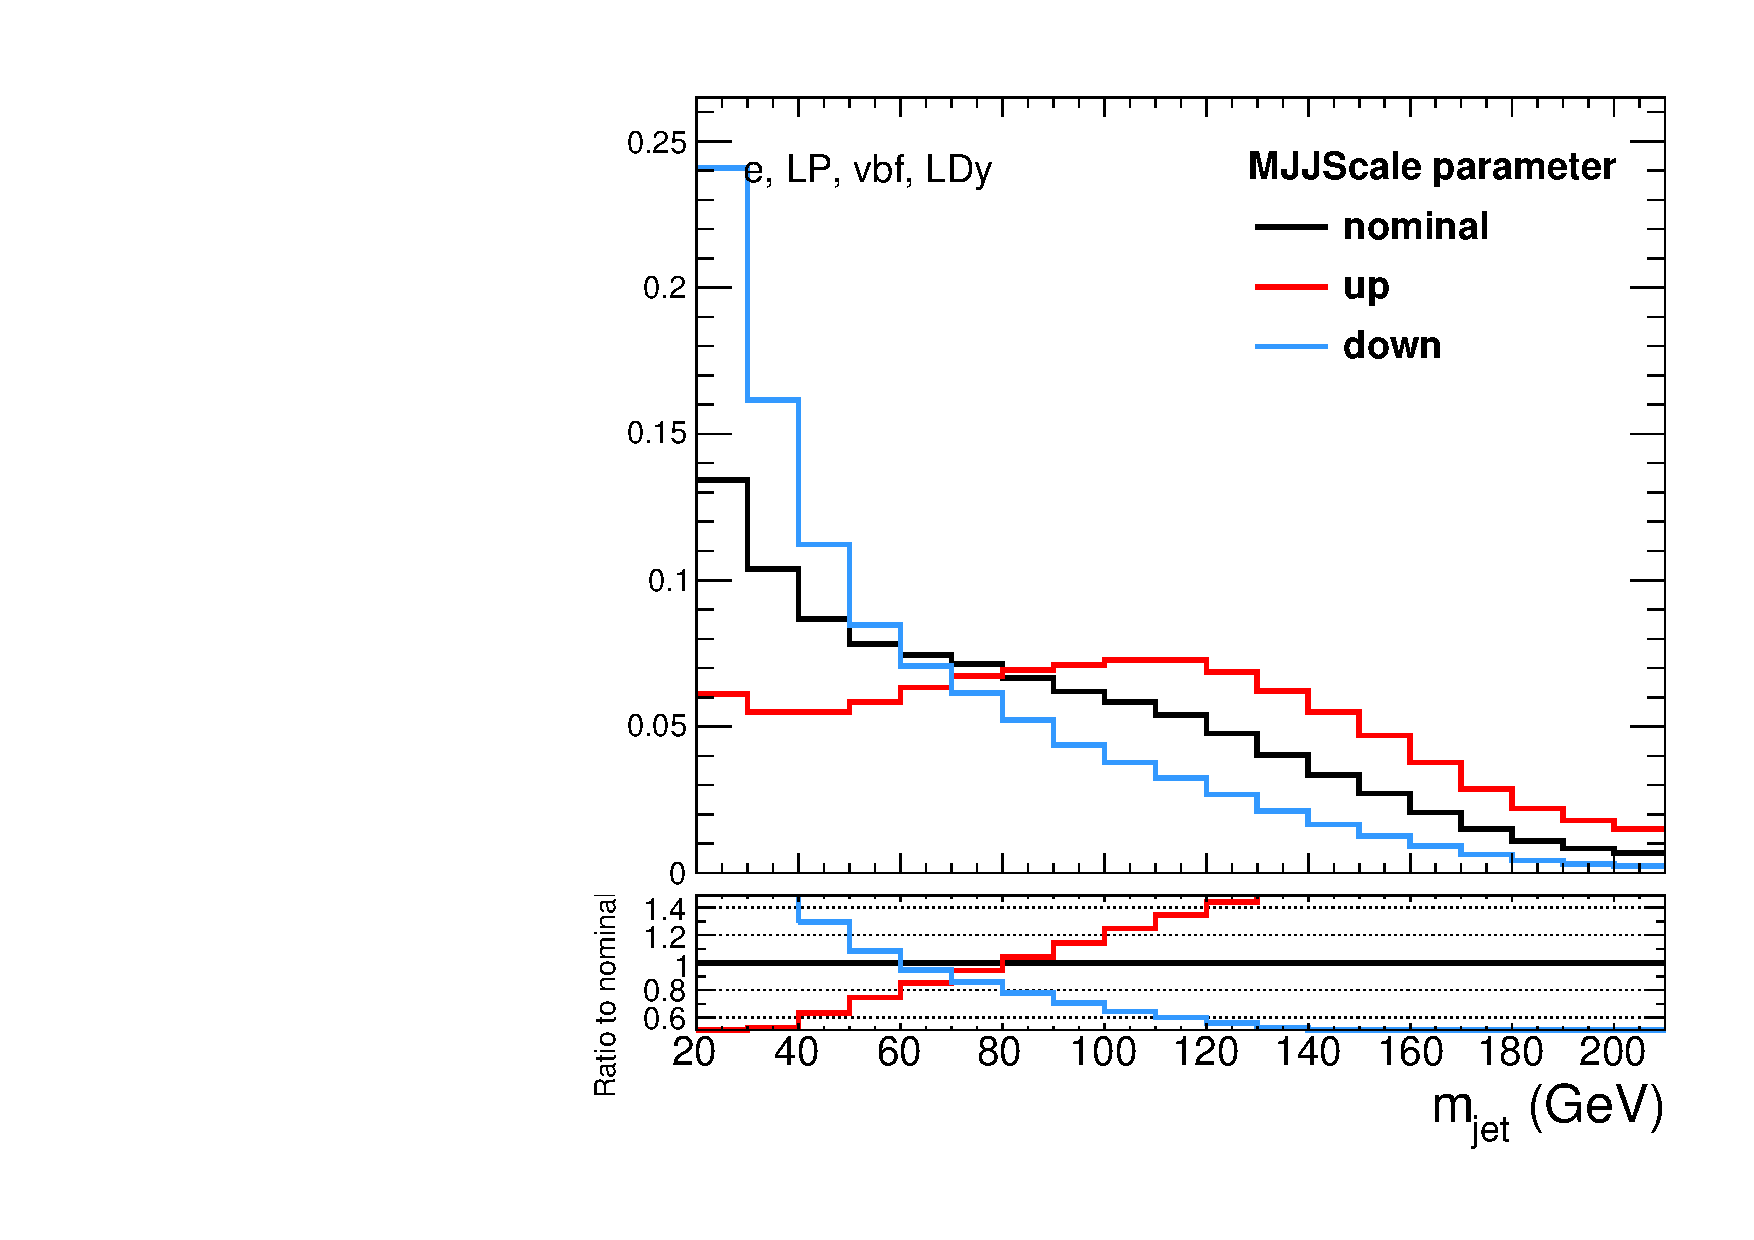
\includegraphics[width=0.21\textwidth]{fig/uncertainties/systs_nonRes_e_LP_vbf_LDy_MJJScale_ProjY.pdf}
  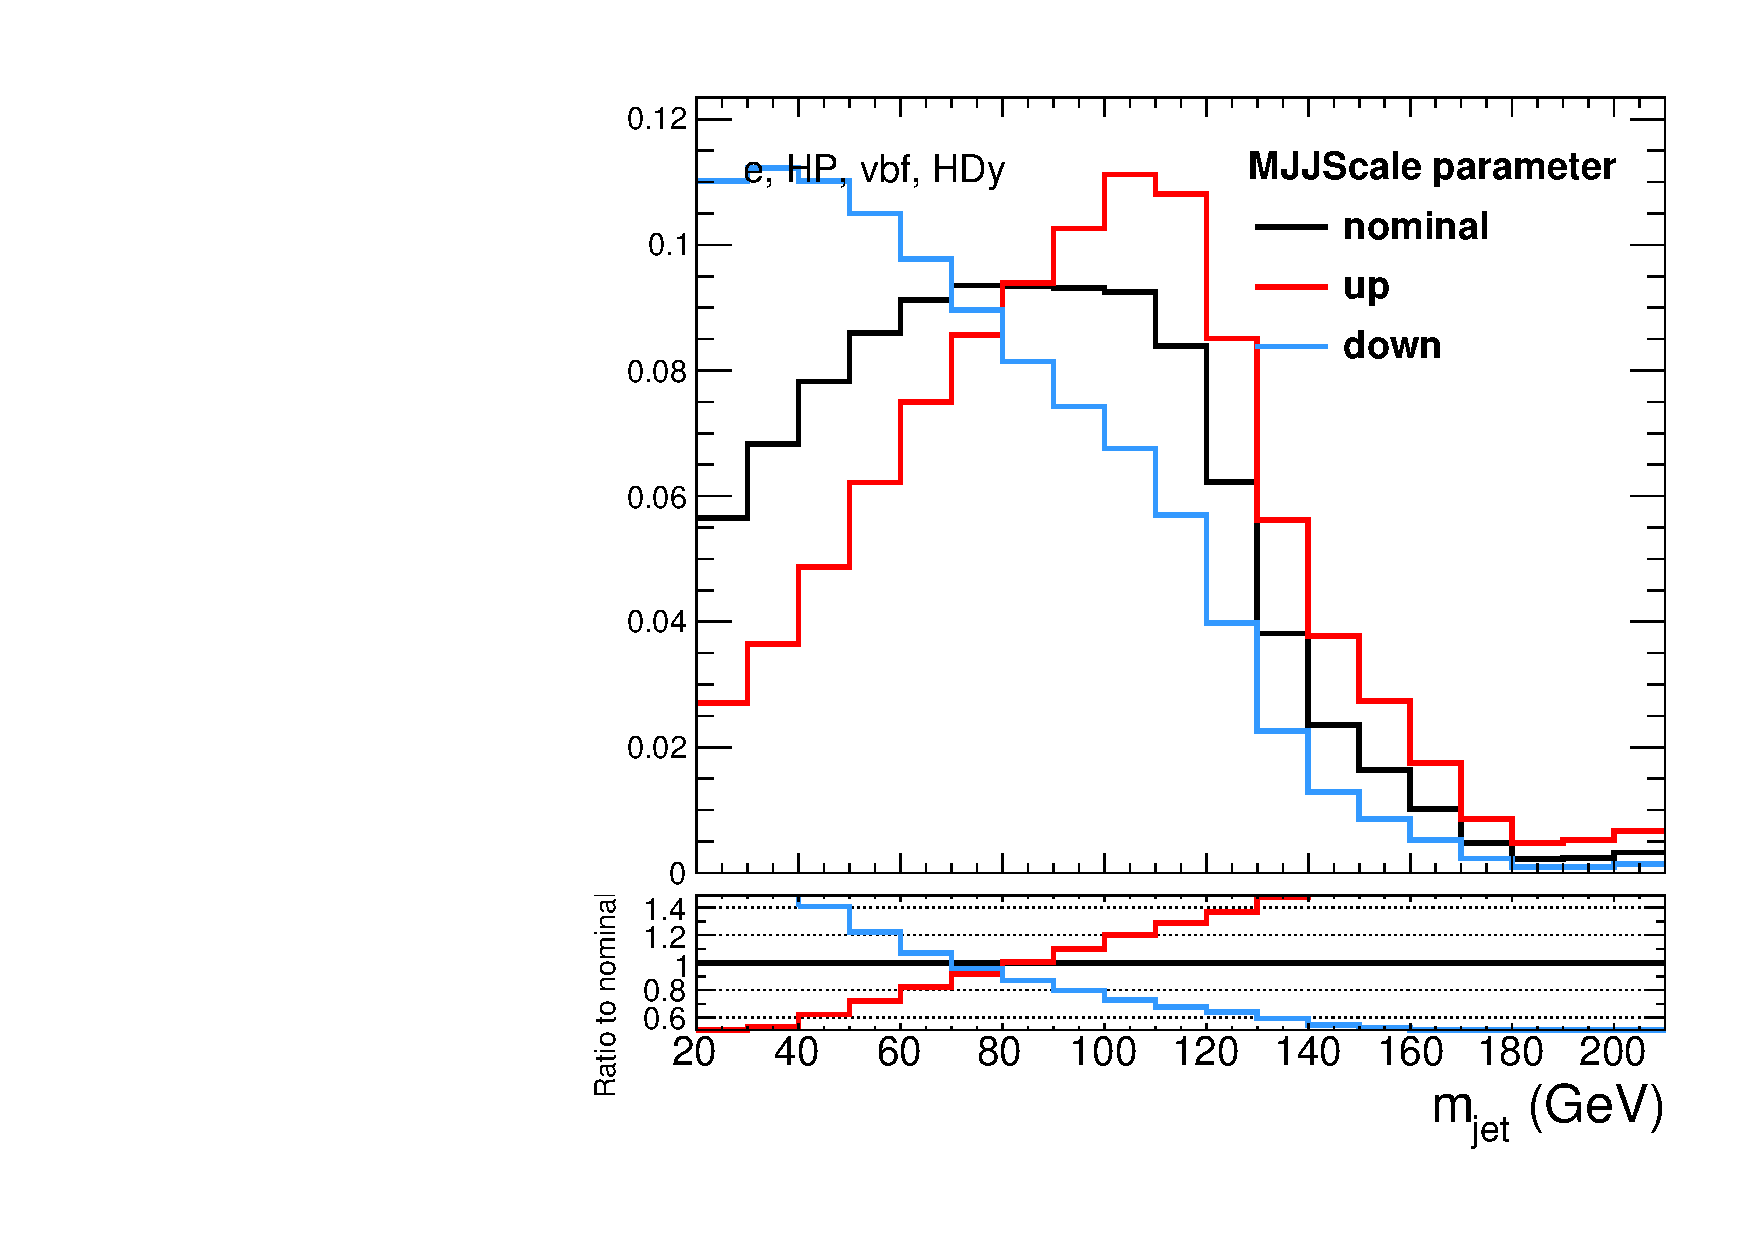
\includegraphics[width=0.21\textwidth]{fig/uncertainties/systs_nonRes_e_HP_vbf_HDy_MJJScale_ProjY.pdf}
  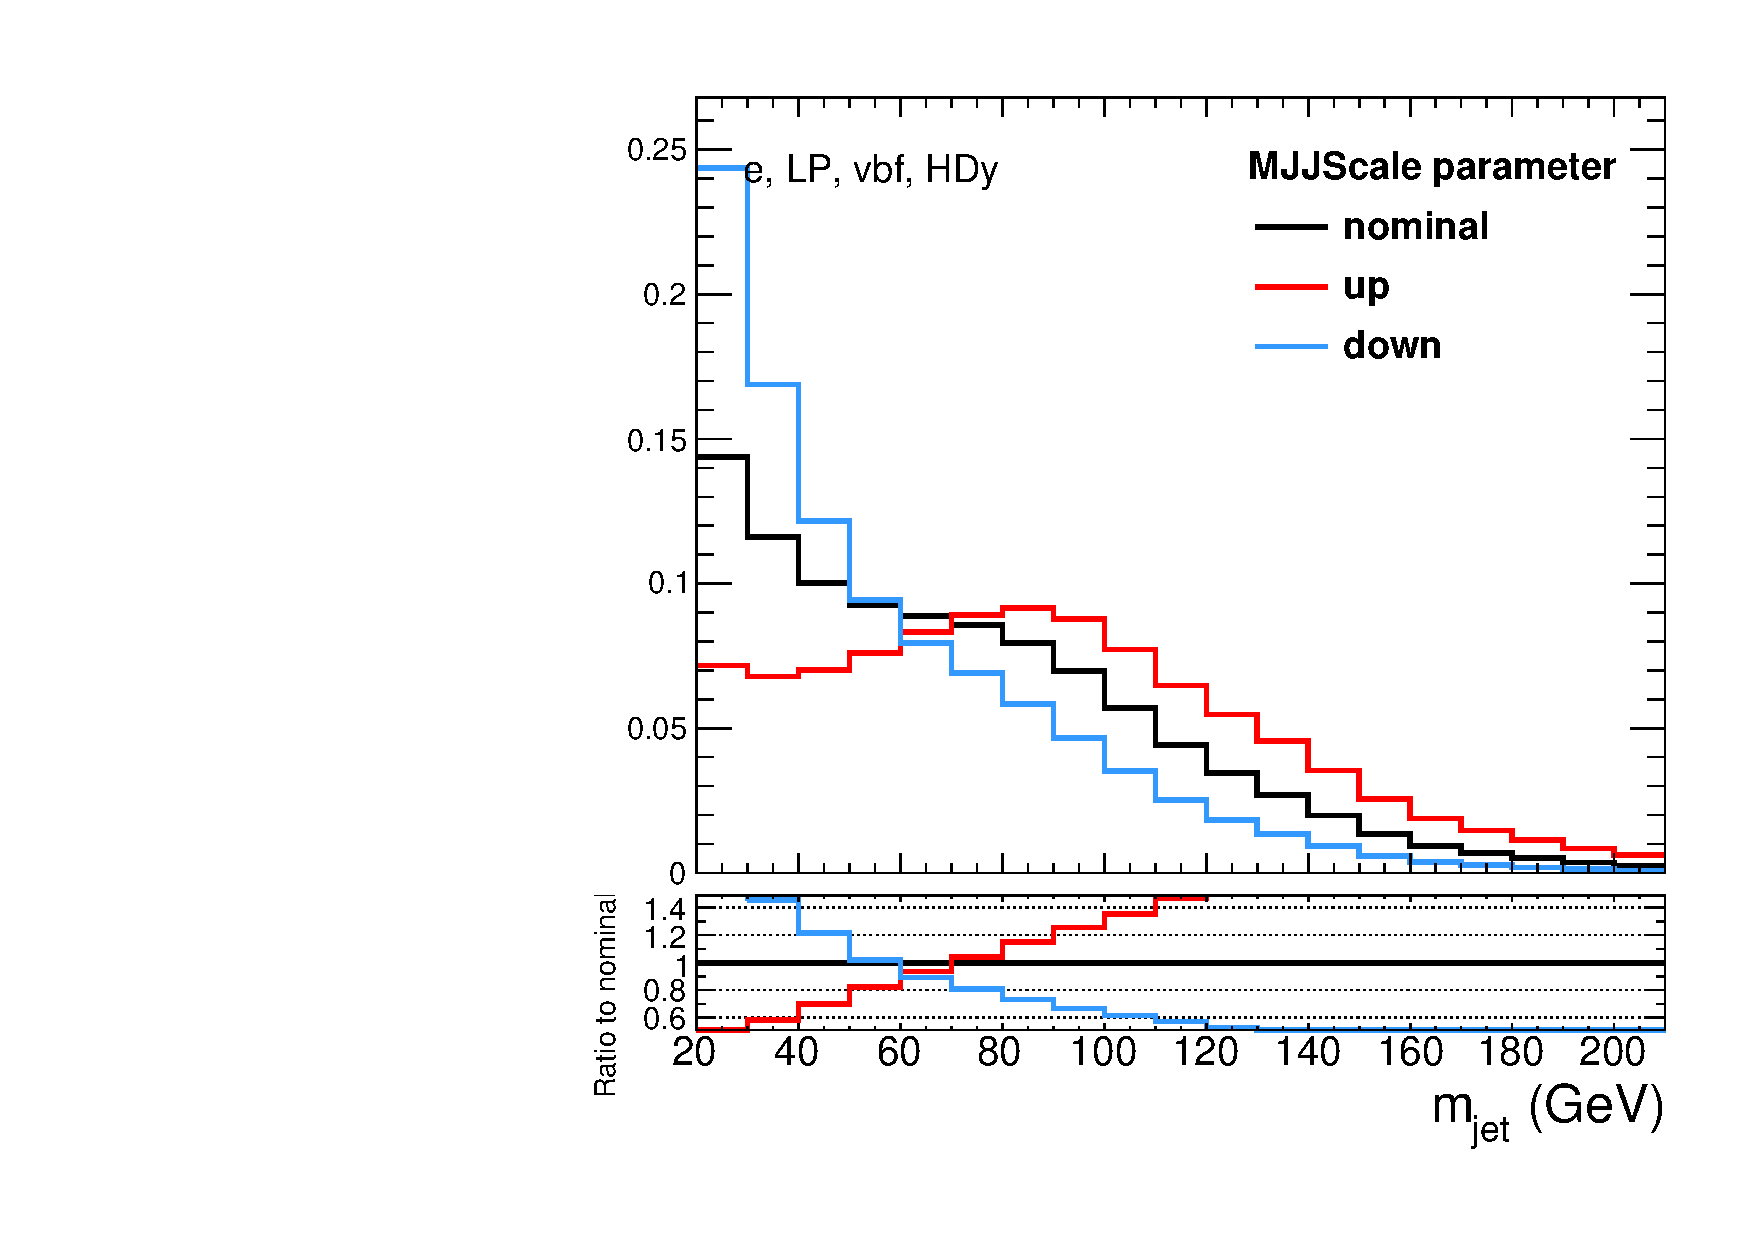
\includegraphics[width=0.21\textwidth]{fig/uncertainties/systs_nonRes_e_LP_vbf_HDy_MJJScale_ProjY.pdf}\\
  \caption{
    Projections of the nominal and alternative shapes of the non-resonant background onto the \MJ dimension obtained from applying $\pm3\sigma$ variations of the \MJ scale uncertainties for the electron channel.
    Columns 1 to 4: HP-LDy, LP-LDy, HP-HDy, LP-HDy.
    Rows 1 to 3: bb, nobb, vbf.
  }
  \label{fig:systNonResMJ_MJJScale}
\end{figure}

\subsection{Resonant Background Shape}

% Resonant conditional shape variation
As with the non-resonant background shapes, we apply a jet \pt spectrum related uncertainty, but with two additional sets of nuisance parameters introduced for the LP categories corresponding to the two \MJ bins used to build the \MVV likelihood.
The HP categories use only one \MJ bin, hence they only have one set of nuisance parameters.
We also apply an uncertainty in the exponent of the power-law function used to populate the high-\MVV region of the template for each category.
These nuisance parameters are also uncorrelated between categories and are uncorrelated between the resonant and non-resonant backgrounds.
Figures~\ref{fig:systResMVV_MVVScale} and \ref{fig:systResMVV_MVVTail} show the nominal and $\pm3\sigma$ alternative 2D shapes projected onto the \MVV dimension for the jet \pt spectrum related and the \MVV power-law exponent uncertainties.

\begin{figure}[htbp]
  \centering
  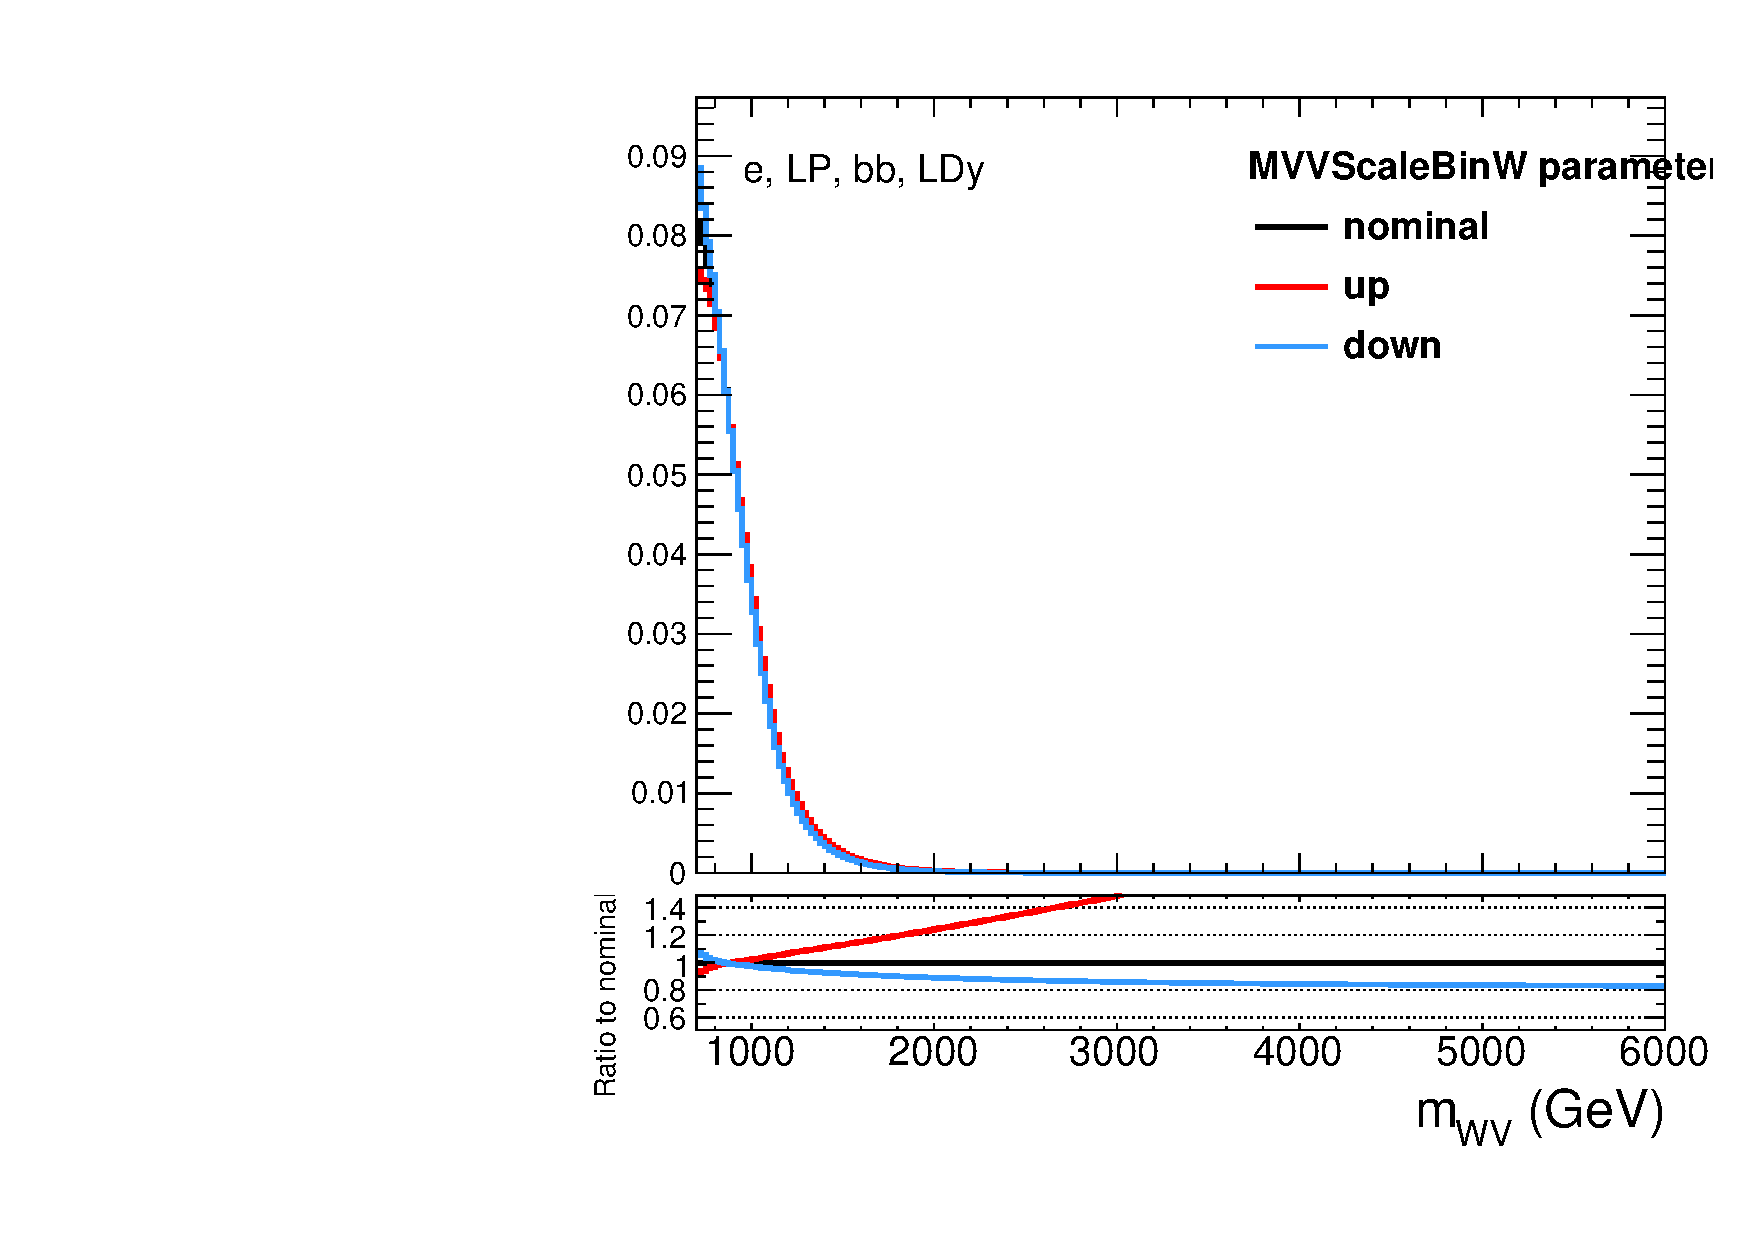
\includegraphics[width=0.21\textwidth]{fig/uncertainties/systs_res_e_LP_bb_LDy_MVVScaleBinW_ProjX.pdf}
  \includegraphics[width=0.21\textwidth]{fig/uncertainties/systs_res_e_LP_bb_HDy_MVVScaleBinW_ProjX.pdf}
  \includegraphics[width=0.21\textwidth]{fig/uncertainties/systs_res_e_LP_bb_LDy_MVVScaleBinTop_ProjX.pdf}
  \includegraphics[width=0.21\textwidth]{fig/uncertainties/systs_res_e_LP_bb_HDy_MVVScaleBinTop_ProjX.pdf}\\
  \includegraphics[width=0.21\textwidth]{fig/uncertainties/systs_res_e_LP_nobb_LDy_MVVScaleBinW_ProjX.pdf}
  \includegraphics[width=0.21\textwidth]{fig/uncertainties/systs_res_e_LP_nobb_HDy_MVVScaleBinW_ProjX.pdf}
  \includegraphics[width=0.21\textwidth]{fig/uncertainties/systs_res_e_LP_nobb_LDy_MVVScaleBinTop_ProjX.pdf}
  \includegraphics[width=0.21\textwidth]{fig/uncertainties/systs_res_e_LP_nobb_HDy_MVVScaleBinTop_ProjX.pdf}\\
  \includegraphics[width=0.21\textwidth]{fig/uncertainties/systs_res_e_LP_vbf_LDy_MVVScaleBinW_ProjX.pdf}
  \includegraphics[width=0.21\textwidth]{fig/uncertainties/systs_res_e_LP_vbf_HDy_MVVScaleBinW_ProjX.pdf}
  \includegraphics[width=0.21\textwidth]{fig/uncertainties/systs_res_e_LP_vbf_LDy_MVVScaleBinTop_ProjX.pdf}
  \includegraphics[width=0.21\textwidth]{fig/uncertainties/systs_res_e_LP_vbf_HDy_MVVScaleBinTop_ProjX.pdf}\\
  \caption{
    Projections of the nominal and alternative shapes of the resonant background onto the \MVV dimension obtained from applying $\pm3\sigma$ variations of the jet \pt spectrum uncertainties for the electron channel.
    Columns 1 to 4: HP-LDy, LP-LDy, HP-HDy, LP-HDy.
    Rows 1 to 3: bb, nobb, vbf.
  }
  \label{fig:systResMVV_MVVScale}
\end{figure}

\begin{figure}[htbp]
  \centering
  \includegraphics[width=0.21\textwidth]{fig/uncertainties/systs_res_e_HP_bb_LDy_MVVTail_ProjX.pdf}
  \includegraphics[width=0.21\textwidth]{fig/uncertainties/systs_res_e_LP_bb_LDy_MVVTail_ProjX.pdf}
  \includegraphics[width=0.21\textwidth]{fig/uncertainties/systs_res_e_HP_bb_HDy_MVVTail_ProjX.pdf}
  \includegraphics[width=0.21\textwidth]{fig/uncertainties/systs_res_e_LP_bb_HDy_MVVTail_ProjX.pdf}\\
  \includegraphics[width=0.21\textwidth]{fig/uncertainties/systs_res_e_HP_nobb_LDy_MVVTail_ProjX.pdf}
  \includegraphics[width=0.21\textwidth]{fig/uncertainties/systs_res_e_LP_nobb_LDy_MVVTail_ProjX.pdf}
  \includegraphics[width=0.21\textwidth]{fig/uncertainties/systs_res_e_HP_nobb_HDy_MVVTail_ProjX.pdf}
  \includegraphics[width=0.21\textwidth]{fig/uncertainties/systs_res_e_LP_nobb_HDy_MVVTail_ProjX.pdf}\\
  \includegraphics[width=0.21\textwidth]{fig/uncertainties/systs_res_e_HP_vbf_LDy_MVVTail_ProjX.pdf}
  \includegraphics[width=0.21\textwidth]{fig/uncertainties/systs_res_e_LP_vbf_LDy_MVVTail_ProjX.pdf}
  \includegraphics[width=0.21\textwidth]{fig/uncertainties/systs_res_e_HP_vbf_HDy_MVVTail_ProjX.pdf}
  \includegraphics[width=0.21\textwidth]{fig/uncertainties/systs_res_e_LP_vbf_HDy_MVVTail_ProjX.pdf}\\
  \caption{
    Projections of the nominal and alternative shapes of the resonant background onto the \MVV dimension obtained from applying $\pm3\sigma$ variations of the high-\MVV power-law tail uncertainties for the electron channel.
    Columns 1 to 4: HP-LDy, LP-LDy, HP-HDy, LP-HDy.
    Rows 1 to 3: bb, nobb, vbf.
  }
  \label{fig:systResMVV_MVVTail}
\end{figure}

% Resonant jet shape variation
For the \MJ dimension of the resonant background, we consider three types of shape uncertainties.
The first two are uncorrelated and modify the mean and width of the fitted DCB functions for the $W$ and top peaks, and they correspond to the nuisance parameters for the soft drop mass scale and resolution.
Meanwhile, the last set of parameters determine the relative normalization of the $W$ and top peaks:
\begin{itemize}
  \item {\bfseries $W$ peak scale and resolution:} 1\% for the scale and 8\% for the resolution.
  We also correct the central values of the scale and resolution for the $W$ peak with factors of 0.989 and 1.08 using the Run 2 values of table~\ref{tab:VScaleRes}.
  The nuisance parameters are uncorrelated between HP and LP categories, but 100\% correlated between the electron and muon channels, the bb, nobb, and vbf categories, and the LDy and HDy categories.
  They are also 100\% correlated to the \MJ scale and resolution parameters of the signal models.
  \item {\bfseries Top peak scale and resolution:} 1\% for the scale and 8\% for the resolution.
  No corrections are made to the parameters of the top peak, and the nuisance parameters are uncorrelated between HP and LP categories, but 100\% correlated between the electron and muon channels, the bb, nobb, and vbf categories, and the LDy and HDy categories.
  \item {\bfseries $W$/top relative normalization:} Fraction of the $W$ peak normalization divided by the sum of the $W$ and top peaks defined such that $\pm40\%$ corresponds to a $\pm3\sigma$ shift.
  These parameters are uncorrelated between categories.
\end{itemize}
Figures~\ref{fig:systResMJ_scaleWY} and \ref{fig:systResMJ_resWY} show the nominal and $\pm3\sigma$ alternative 2D shapes projected onto the \MJ dimension for the $W$ peak and scale uncertainties.
Meanwhile, figures~\ref{fig:systResMJ_scaleTopY} and \ref{fig:systResMJ_scaleTopY} show the nominal and $\pm3\sigma$ alternative 2D shapes projected onto the \MJ dimension for the top peak and scale uncertainties.
Finally, figure~\ref{fig:systResMJ_fractionY} shows the nominal and $\pm3\sigma$ alternative 2D shapes projected onto the \MJ dimension for the $W$ and top relative normalization uncertainty.

\begin{figure}[htbp]
  \centering
  \includegraphics[width=0.21\textwidth]{fig/uncertainties/systs_res_e_HP_bb_LDy_scaleWY_ProjY.pdf}
  \includegraphics[width=0.21\textwidth]{fig/uncertainties/systs_res_e_LP_bb_LDy_scaleWY_ProjY.pdf}
  \includegraphics[width=0.21\textwidth]{fig/uncertainties/systs_res_e_HP_bb_HDy_scaleWY_ProjY.pdf}
  \includegraphics[width=0.21\textwidth]{fig/uncertainties/systs_res_e_LP_bb_HDy_scaleWY_ProjY.pdf}\\
  \includegraphics[width=0.21\textwidth]{fig/uncertainties/systs_res_e_HP_nobb_LDy_scaleWY_ProjY.pdf}
  \includegraphics[width=0.21\textwidth]{fig/uncertainties/systs_res_e_LP_nobb_LDy_scaleWY_ProjY.pdf}
  \includegraphics[width=0.21\textwidth]{fig/uncertainties/systs_res_e_HP_nobb_HDy_scaleWY_ProjY.pdf}
  \includegraphics[width=0.21\textwidth]{fig/uncertainties/systs_res_e_LP_nobb_HDy_scaleWY_ProjY.pdf}\\
  \includegraphics[width=0.21\textwidth]{fig/uncertainties/systs_res_e_HP_vbf_LDy_scaleWY_ProjY.pdf}
  \includegraphics[width=0.21\textwidth]{fig/uncertainties/systs_res_e_LP_vbf_LDy_scaleWY_ProjY.pdf}
  \includegraphics[width=0.21\textwidth]{fig/uncertainties/systs_res_e_HP_vbf_HDy_scaleWY_ProjY.pdf}
  \includegraphics[width=0.21\textwidth]{fig/uncertainties/systs_res_e_LP_vbf_HDy_scaleWY_ProjY.pdf}\\
  \caption{
    Projections of the nominal and alternative shapes of the resonant background onto the \MJ dimension obtained from applying $\pm3\sigma$ variations of the $W$ peak scale uncertainties for the electron channel.
    Columns 1 to 4: HP-LDy, LP-LDy, HP-HDy, LP-HDy.
    Rows 1 to 3: bb, nobb, vbf.
  }
  \label{fig:systResMJ_scaleWY}
\end{figure}

\begin{figure}[htbp]
  \centering
  \includegraphics[width=0.21\textwidth]{fig/uncertainties/systs_res_e_HP_bb_LDy_resWY_ProjY.pdf}
  \includegraphics[width=0.21\textwidth]{fig/uncertainties/systs_res_e_LP_bb_LDy_resWY_ProjY.pdf}
  \includegraphics[width=0.21\textwidth]{fig/uncertainties/systs_res_e_HP_bb_HDy_resWY_ProjY.pdf}
  \includegraphics[width=0.21\textwidth]{fig/uncertainties/systs_res_e_LP_bb_HDy_resWY_ProjY.pdf}\\
  \includegraphics[width=0.21\textwidth]{fig/uncertainties/systs_res_e_HP_nobb_LDy_resWY_ProjY.pdf}
  \includegraphics[width=0.21\textwidth]{fig/uncertainties/systs_res_e_LP_nobb_LDy_resWY_ProjY.pdf}
  \includegraphics[width=0.21\textwidth]{fig/uncertainties/systs_res_e_HP_nobb_HDy_resWY_ProjY.pdf}
  \includegraphics[width=0.21\textwidth]{fig/uncertainties/systs_res_e_LP_nobb_HDy_resWY_ProjY.pdf}\\
  \includegraphics[width=0.21\textwidth]{fig/uncertainties/systs_res_e_HP_vbf_LDy_resWY_ProjY.pdf}
  \includegraphics[width=0.21\textwidth]{fig/uncertainties/systs_res_e_LP_vbf_LDy_resWY_ProjY.pdf}
  \includegraphics[width=0.21\textwidth]{fig/uncertainties/systs_res_e_HP_vbf_HDy_resWY_ProjY.pdf}
  \includegraphics[width=0.21\textwidth]{fig/uncertainties/systs_res_e_LP_vbf_HDy_resWY_ProjY.pdf}\\
  \caption{
    Projections of the nominal and alternative shapes of the resonant background onto the \MJ dimension obtained from applying $\pm3\sigma$ variations of the $W$ peak resolution uncertainties for the electron channel.
    Columns 1 to 4: HP-LDy, LP-LDy, HP-HDy, LP-HDy.
    Rows 1 to 3: bb, nobb, vbf.
  }
  \label{fig:systResMJ_resWY}
\end{figure}

\begin{figure}[htbp]
  \centering
  \includegraphics[width=0.21\textwidth]{fig/uncertainties/systs_res_e_HP_bb_LDy_scaleTopY_ProjY.pdf}
  \includegraphics[width=0.21\textwidth]{fig/uncertainties/systs_res_e_LP_bb_LDy_scaleTopY_ProjY.pdf}
  \includegraphics[width=0.21\textwidth]{fig/uncertainties/systs_res_e_HP_bb_HDy_scaleTopY_ProjY.pdf}
  \includegraphics[width=0.21\textwidth]{fig/uncertainties/systs_res_e_LP_bb_HDy_scaleTopY_ProjY.pdf}\\
  \includegraphics[width=0.21\textwidth]{fig/uncertainties/systs_res_e_HP_nobb_LDy_scaleTopY_ProjY.pdf}
  \includegraphics[width=0.21\textwidth]{fig/uncertainties/systs_res_e_LP_nobb_LDy_scaleTopY_ProjY.pdf}
  \includegraphics[width=0.21\textwidth]{fig/uncertainties/systs_res_e_HP_nobb_HDy_scaleTopY_ProjY.pdf}
  \includegraphics[width=0.21\textwidth]{fig/uncertainties/systs_res_e_LP_nobb_HDy_scaleTopY_ProjY.pdf}\\
  \includegraphics[width=0.21\textwidth]{fig/uncertainties/systs_res_e_HP_vbf_LDy_scaleTopY_ProjY.pdf}
  \includegraphics[width=0.21\textwidth]{fig/uncertainties/systs_res_e_LP_vbf_LDy_scaleTopY_ProjY.pdf}
  \includegraphics[width=0.21\textwidth]{fig/uncertainties/systs_res_e_HP_vbf_HDy_scaleTopY_ProjY.pdf}
  \includegraphics[width=0.21\textwidth]{fig/uncertainties/systs_res_e_LP_vbf_HDy_scaleTopY_ProjY.pdf}\\
  \caption{
    Projections of the nominal and alternative shapes of the resonant background onto the \MJ dimension obtained from applying $\pm3\sigma$ variations of the top peak scale uncertainties for the electron channel.
    Columns 1 to 4: HP-LDy, LP-LDy, HP-HDy, LP-HDy.
    Rows 1 to 3: bb, nobb, vbf.
  }
  \label{fig:systResMJ_scaleTopY}
\end{figure}

\begin{figure}[htbp]
  \centering
  \includegraphics[width=0.21\textwidth]{fig/uncertainties/systs_res_e_HP_bb_LDy_resTopY_ProjY.pdf}
  \includegraphics[width=0.21\textwidth]{fig/uncertainties/systs_res_e_LP_bb_LDy_resTopY_ProjY.pdf}
  \includegraphics[width=0.21\textwidth]{fig/uncertainties/systs_res_e_HP_bb_HDy_resTopY_ProjY.pdf}
  \includegraphics[width=0.21\textwidth]{fig/uncertainties/systs_res_e_LP_bb_HDy_resTopY_ProjY.pdf}\\
  \includegraphics[width=0.21\textwidth]{fig/uncertainties/systs_res_e_HP_nobb_LDy_resTopY_ProjY.pdf}
  \includegraphics[width=0.21\textwidth]{fig/uncertainties/systs_res_e_LP_nobb_LDy_resTopY_ProjY.pdf}
  \includegraphics[width=0.21\textwidth]{fig/uncertainties/systs_res_e_HP_nobb_HDy_resTopY_ProjY.pdf}
  \includegraphics[width=0.21\textwidth]{fig/uncertainties/systs_res_e_LP_nobb_HDy_resTopY_ProjY.pdf}\\
  \includegraphics[width=0.21\textwidth]{fig/uncertainties/systs_res_e_HP_vbf_LDy_resTopY_ProjY.pdf}
  \includegraphics[width=0.21\textwidth]{fig/uncertainties/systs_res_e_LP_vbf_LDy_resTopY_ProjY.pdf}
  \includegraphics[width=0.21\textwidth]{fig/uncertainties/systs_res_e_HP_vbf_HDy_resTopY_ProjY.pdf}
  \includegraphics[width=0.21\textwidth]{fig/uncertainties/systs_res_e_LP_vbf_HDy_resTopY_ProjY.pdf}\\
  \caption{
    Projections of the nominal and alternative shapes of the resonant background onto the \MJ dimension obtained from applying $\pm3\sigma$ variations of the top peak resolution uncertainties for the electron channel.
    Columns 1 to 4: HP-LDy, LP-LDy, HP-HDy, LP-HDy.
    Rows 1 to 3: bb, nobb, vbf.
  }
  \label{fig:systResMJ_resTopY}
\end{figure}

\begin{figure}[htbp]
  \centering
  \includegraphics[width=0.21\textwidth]{fig/uncertainties/systs_res_e_HP_bb_LDy_fractionY_ProjY.pdf}
  \includegraphics[width=0.21\textwidth]{fig/uncertainties/systs_res_e_LP_bb_LDy_fractionY_ProjY.pdf}
  \includegraphics[width=0.21\textwidth]{fig/uncertainties/systs_res_e_HP_bb_HDy_fractionY_ProjY.pdf}
  \includegraphics[width=0.21\textwidth]{fig/uncertainties/systs_res_e_LP_bb_HDy_fractionY_ProjY.pdf}\\
  \includegraphics[width=0.21\textwidth]{fig/uncertainties/systs_res_e_HP_nobb_LDy_fractionY_ProjY.pdf}
  \includegraphics[width=0.21\textwidth]{fig/uncertainties/systs_res_e_LP_nobb_LDy_fractionY_ProjY.pdf}
  \includegraphics[width=0.21\textwidth]{fig/uncertainties/systs_res_e_HP_nobb_HDy_fractionY_ProjY.pdf}
  \includegraphics[width=0.21\textwidth]{fig/uncertainties/systs_res_e_LP_nobb_HDy_fractionY_ProjY.pdf}\\
  \includegraphics[width=0.21\textwidth]{fig/uncertainties/systs_res_e_HP_vbf_LDy_fractionY_ProjY.pdf}
  \includegraphics[width=0.21\textwidth]{fig/uncertainties/systs_res_e_LP_vbf_LDy_fractionY_ProjY.pdf}
  \includegraphics[width=0.21\textwidth]{fig/uncertainties/systs_res_e_HP_vbf_HDy_fractionY_ProjY.pdf}
  \includegraphics[width=0.21\textwidth]{fig/uncertainties/systs_res_e_LP_vbf_HDy_fractionY_ProjY.pdf}\\
  \caption{
    Projections of the nominal and alternative shapes of the resonant background onto the \MJ dimension obtained from applying $\pm3\sigma$ variations of the $W$ and top relative normalizations for the electron channel.
    Columns 1 to 4: HP-LDy, LP-LDy, HP-HDy, LP-HDy.
    Rows 1 to 3: bb, nobb, vbf.
  }
  \label{fig:systResMJ_fractionY}
\end{figure}
